\documentclass[a4paper]{report}


%%% Packages
\usepackage{fancyhdr}
\usepackage[raggedright]{titlesec}
\pagestyle{fancy}
\usepackage{xcolor}
\usepackage[footnote, draft, silent, nomargin]{fixme}
\usepackage[utf8]{inputenc}

\usepackage{graphicx}



%%% Util commands
\newcommand\TODO[1]{\textcolor{red}{#1}}



\title{Barricelli}
\date{\today}
\author{Emil Taylor Bye
     \and Fedor Fadeev
     \and Sigve Sebastian Farstad
     \and Péter Gombos
     \and Rune Holmgren
     \and Torbjørn Langland
     \and Per Thomas Lundal
     \and Odd Magnus Trondrud
     \and Bjørn Åge Tungesvik
     \and Eirik Flogard
}

\lhead{Computer Project}
\chead{Barricelli}
\rhead{Performance Group}
\lfoot{}
\cfoot{\thepage}
\rfoot{}

\begin{document}
\newglossaryentry{barricelli}
{
name=Barricelli,
description={is the name of the genetic algorithm-solving MIMD computer designed as a solution for the project documented in this report. Barricelli is also the name of a famous Norwegian-Italian mathematician, after whom the computer is named}
}

\newglossaryentry{galapagos}
{
name=Galapagos,
description={is the name of the instruction set architecture designed for the Barricelli computer}
}

\newglossaryentry{galapagos assembler}
{
name=Galapagos Assembler,
description={The assembler for Galapagos Assembly written in Python.}
}

\newglossaryentry{MIMD}
{
name=MIMD,
description={Multiple Instruction, Multiple Data}
}

\newglossaryentry{individual}
{
name=individual,
description={A single, feasible solution to a hard problem in genetic algorithms.}
}

\newglossaryentry{MIPS}
{
name=MIPS,
description={\todo{description}}
}

\newglossaryentry{RISC}
{
name=RISC,
description={\todo{description}}
}

\newglossaryentry{nop}
{
name=nop,
description={The general nop assembly instruction \todo{description}}
}

\newglossaryentry{DSP slice}
{
name=DSP slice,
description={\todo{description}}
}

\newglossaryentry{FPGA}
{
name=FPGA,
description={\todo{description}}
}

\newglossaryentry{LUT}
{
name=LUT,
description={\todo{description}}
}

\newglossaryentry{SCU}
{
name=SCU,
description={is the EFM32 microcontroller which is used as a System control unit}
}

\newglossaryentry{VHDL}
{
name=VHDL,
description={is the programming language in which the processor in implemented. VHDL is short for \gls{VHSIC} Hardware Description Language}
}

\newglossaryentry{VHSIC}
{
name=VHSIC,
description={is short for Very High-Speed Integrated Circuit}
}

\newglossaryentry{isim}
{
name=isim
description={isim is a simulator part of the Xilinx developer suite.}

\pagenumbering{roman}

\ThisCenterWallPaper{1}{fig/barricelli-title-page.pdf}

\newpage
\thispagestyle{empty}
\mbox{}
\newpage

\begin{abstract}
	This is an abstract.
As it turns out, the project was a success.

Barricelli, the computer designed in this project, is a general purpose MIMD computer which is equipped with specialized hardware for high performance computation of hard problems using genetic algorithms.

\todo{write a good abstract (but do not make it too abstract)}

\end{abstract}

\thispagestyle{empty}
\section*{Acknowledgements}
A big thank you is extended to the following for invaluable help and guidance during this project:

\begin{description}
\item[Gunnar Tufte] for ... having long hair
\item[Yaman Umuroglu] for ...
\item[Stephano Nichele] for ...
\item[Odd Rune S. Lykkebø] for ...
\item[Navn Navnesen] for being a hero.
\item[The other group] for company in the lab during the late hours of the night.
\item[Somebody] for 3D-printing, perhaps?
\item[Teknisk Gruppe, IDI] for coffee related accessories
\todo{more?}
\end{description}

% set to 3 bacause abstact and acknowledgement comes before it
\setcounter{page}{3}

\tableofcontents
\newpage

\listoffigures
\listoftables
\listofalgorithms
\renewcommand{\lstlistlistingname}{List of Listings}

\newpage
\setcounter{page}{1}
\pagenumbering{arabic}

\part{Introduction and Background}

\chapter{Introduction}
	This report presents a solution to ``Task: Construct a Multiple Program, Multiple Data'' of the autumn 2013 course TDT4295 Computer Design Project at the Norwegian University of Science and Technology (NTNU).

The course is a single-task, whole-semester course in which a group of students collaborate to design and implement a computer in hardware.
The computer presented in this report was made by a group of 10 students.

This report details the design and implementation of \Gls{barricelli}, the solution computer designed for this project.
The design process is also documented in this report.

\section{Assignment}


This section details the assignment given for the project.

\subsection{Assignment Text}
\label{subsection:assignment-text}

\begin{quote}

\begin{center}
TDT4295 Computer Design Project

Assignment Text

2013 
\end{center}
 
\textbf{Task: Construct a Multiple Program, Multiple Data}

The performance increase available from harvesting Instruction Level Parallelism (ILP) from the serial instruction stream is limited because we have reached the maximum power consumption that can be handled without expensive cooling solutions.
Consequently, there is a significant interest in single-chip parallel processor solutions.
The processor cores in commercial multi-core chips are conventional designs and therefore reasonably complex.
In this work, your task is to design a multiprocessor,Multiple Instruction, Multiple Data streams (MIMD).
A processor classified MIMD include a multiple-instruction stream organizations.
Such processors can executing different instructions, i.e. minimum 2 independent programs, on different (independent) data.

The task also include that a suitable application is chosen to demonstrate the processor.
Your processor will be implemented on an FPGA, and you are free to choose how to realize your MIMD computer architecture.
The system should be shown to work with a suitable application.
Studying the architecture of the Cell processor, or in general multi-core processors, can be a good starting point.
And a final tip; Keep it simple, as simple as possible, but not simpler.

Due to a large number of students this year, we will divide the work into two independent projects: a) Performance and b) Energy efficiency.
The goal of group a) is to achieve maximum performance while group b) should try to balance performance and energy.
The reports from both groups should include an evaluation of prototype performance and energy consumption.

\textbf{Additional requirements}

The unit must utilize an Energy Micro microcontroller and a Xilinx FPGA.
The budget is 10.000 NOK, which must cover components and PCB production.
The unit design must adhere to the limits set by the course staff at any given time.
Deadlines are given in a separate time schedule.

\textbf{Evaluation}

The project is evaluated based on the project report and an oral presentation of the work as well as a prototype demonstration.
One grade will be given to the group as a whole, unless there are significant variations in the amount of effort put into the project. 
\cite{assignment-text}
\end{quote}

\subsection{Interpretation}

There are many different ways to solve the task described in the assignment text in subsection \vref{subsection:assignment-text}.
To give direction to the project, an application for the solution computer was chosen at an early stage.
The application chosen for the solution computer presented in this report is a generic solver of optimization and approximation problems using genetic algorithms.
The main goal for the project is to be able to implement the generic solver by exploiting the principles of the MIMD architecture scheme.

As mentioned in the assignment text, there are two groups working on the computer design project, making two different computers.
The solution presented in this report is the solution of the group that was to achieve maximum performance.


\section{Requirements}

This section describes the requirements for this assignment, and explains the rationale behind them.
The functional requirements for the project are listed in table \vref{table:functional-requirements}.
The non-functional requirements for the project are listed in table \vref{table:non-functional-requirements}.

 \subsection{Functional Requirements}

 \begin{table}[H]
 \begin{center}
 \begin{tabular}{| l | p{7cm} | l |}
 \hline
 Requirement & Description & Priority\\
 \hline
 FR1 & The system should be a MIMD computer. & High \\
 FR2 & The system should be a general computer. & High \\
 FR3 & The system should be able to solve hard problems using genetic alogorithms. & High \\
 FR4 & The system should be able to receive instructions and data from an external entity. & High \\
 FR5 & The system should be able to send data to an external entity. & High \\
 FR6 & The product should have maximized performance rather than energy-efficiency. & Medium \\
 FR7 & The instruction set should contain custom made instructions for faster execution of genetic algorithms. & Medium \\
 \hline
 \end{tabular}
 \caption{Functional Requirements}
 \label{table:functional-requirements}
 \end{center}
 \end{table}

\subsubsection{FR1}

FR1 in table \vref{table:functional-requirements} states that the system should be a MIMD computer.
This requirement is set as the main requirement in the assigment text, and is therefore a high prority requirement.

\subsubsection{FR2}

 FR2 in table \vref{table:functional-requirements} states that the system should be a general computer.
 That means that the computer should be Turing Complete, which implies that it can solve any computable problem.
 This was set as a goal because it enables the computation of fitness values of genetic individuals for arbitrary problems. 
 Because this requirement is a necessity for the chosen genetic algorithm solver application, is has a high priority.

\subsubsection{FR3}

FR3 in table \vref{table:functional-requirements} states that the system should be able to solve hard problems using genetic algorithms.
(For a definition of a hard problem, see \vref{ga-algorithms}.)
This is the application that was chosen for the computer, and is its \textit{raison d'être}. 
Therefore, this requirement also has a high priority.

\subsubsection{FR4}

FR4 in table \vref{table:functional-requirements} states that the system should be able to receive instructions and data from an external entity.
Without this requirement fulfilled, it is impossible to program, configure or run the program with other instructions or data than what comes `pre-loaded', so to speak.
That would make the system pretty useless.
For this reason, this requirement also has a high priority.

\subsubsection{FR5}

FR5 in table \vref{table:functional-requirements} states that the system should be able to send data to an external entity.
This is needed for the computer to return its computed results to a user.
Again, without this requirement, the computer would be quite useless.
Of course, that means that this requirement also must have a high priority.

\subsubsection{FR6}

FR6 in table \vref{table:functional-requirements} states that the product should have maximized performance rather than energy-efficiency.
This requirement is set from the assignment text.
Although this is an important requirement, not meeting it does not imply that the solution computer is completely useless.
A less-than-optimally performant computer will still be able to solve hard problems, even if it will do it slower.
Because of this, even though this requirement is specifically mentioned in the assignment text, this requirement is assigned a medium priority.

\subsubsection{FR7}

FR7 in table \vref{table:functional-requirements} states that the instruction set should contain custom made instructions for faster execution of genetic algorithms.
This requirement is set because it helps setting the focus on high performance.
Another reason for this requirement is that it makes high performance genetic algorithm programming easier for developers using the computer.
This greatly increases the usability of the computer.

\subsection{Non-functional Requirements}

\begin{table}[H]
\begin{center}
\begin{tabular}{| l | p{7cm} | l |}
\hline
Requirement & Description & Priority \\
\hline
NFR1 & The system should be built so that the soldering process does not take longer then 8 hours when done by hand. & High \\
NFR2 & The system should use a Xilinx FPGA. & High\\
NFR3 & The system should use an "Energy Micro" microcontroller. & High \\
NFR4 & The system should not cost more than 10000 NOK. & High \\
NFR5 & A report detailing the product and process. & High \\
NFR6 & A working demo program running a genetic algorithm. & Medium \\
NFR7 & The system should have a 3D-printed case. & Low \\
\hline
\end{tabular}
\caption{Non-functional Requirements}
\label{table:non-functional-requirements}
\end{center}
\end{table}

\subsubsection{NFR1}

NFR1 in table \vref{table:non-functional-requirements} states that the system should be built so that soldering does not take longer than 8 hours when done by hand.
This would also include time consumed by baking ball grid array (BGA) components.
This requirement is included because hand-soldering and simple BGA baking are the fabrication techniques readily available to the group without incurring prohibitively large costs, and is therefore a high priority requirement.

\subsubsection{NFR2}

NFR2 in table \vref{table:non-functional-requirements} states that the system should use a Xilinx FPGA.
The assignment text requires that a Xilinx FPGA should be used~\cite{assignment-text}, and the Spartan-6 was chosen.
This is a high priority requirement. 

\subsubsection{NFR3}

NFR3 in table \vref{table:non-functional-requirements} states that the system should use an "Energy Micro" microcontroller~\cite{assignment-text}.
The microcontroller is needed in order to communicate properly with the FPGA and is a high priority requirement.


\subsubsection{NFR4}

NFR4 in table \vref{table:non-functional-requirements} states that the system should not cost more than 10000 NOK.
This is a requirement specified in the assignment text~\cite{assignment-text}, and is therefore a high priority requirement.

\subsubsection{NFR5}

NFR5 in table \vref{table:non-functional-requirements} states that there should be a report detailing the product and process.
This requirement is perhaps the most important requirement, as all the other work would have been for nothing if it were not documented for others to see.
In addition, the assignment text states that the project will be evaluated partially based on the report~\cite{assignment-text}.
This makes this requirement a high priority requirement.

\subsubsection{NFR6}

NFR6 in table \vref{table:non-functional-requirements} states that there should be a working demo program running a genetic algorithm on the system computer.
Although this requirement is also specified in the assignment text, it is set for demonstration purposes.
If a working demo program is not produced, it does not imply that the solution computer is defective.
Because of this, this requirement has a medium priority.

\subsubsection{NFR7}

NFR7 in table \vref{table:non-functional-requirements} states that the system should have a 3D-printed case.
This requirement has a low priority, as, while it looks good, provides protective cover for the computer, and increases usability, it is not crucial for making the computer work.



\section{Deliverables}

 \begin{table}[H]
 \begin{center}
 \begin{tabular}{| l | p{9cm} |}
 \hline
 Deliverable & Description \\
 \hline
 D1 & A functioning version of the computer, with the processor running on an FPGA.\\
 D2 & A working assembler for the instruction set.\\
 D3 & A working demo program running a genetic algorithm.\\
 D3 & A report detailing the product and process.\\
 \hline
 \end{tabular}
 \caption{Deliverables}
 \label{table:deliverables}
 \end{center}
 \end{table}

A deliverable is a tangible or intangible object produced as a result of a project that is intended to be delivered to an other party.
In this case, the deliverables are what this group is handing in as a solution to the assignment stated in section \vref{subsection:assignment-text}.
An overview of the deliverables for this project can be found in table \vref{table:deliverables}.
Here follows a short description of each deliverable.

\subsubsection{D1}

D1 in table \vref{table:deliverables} is the physical manifestation of the Barricelli computer that was designed for this project.

\subsubsection{D2}

D2 in table \vref{table:deliverables} is Galapagos Assembler, a modular \gls{galapagos} assembler written in python.

\subsubsection{D3}

D3 in table \vref{table:deliverables} is a collection of programs written in galapagos assembly for the Barricelli computer, demonstrating its usefulness as a genetics algorithm solver, and also as a general computer.

\subsubsection{D4}

D4 in table \vref{table:deliverables} is this report.



\section{About the Name}

Barricelli is the name of the solution computer presented in this report.
The computer is named after Nils Aall Barricelli, who was a Norwegian-Italian 20th century mathematician.
Barricelli the mathematician was a pioneer in artificial life research, and he performed early computer-assisted experiments in the symbiogenesis and evolution fields.
It is in recognition of Barricelli the mathematicians's groundbreaking seminal work that Barricelli the computer takes its name.
\cite{barricelli-paper}


\section{Structure of this Report}

This report is structured as follows:

Chapter 1 introduces the assignment and its interpretation. 
It also details the goals and requirements set for the project.

Chapter 2 aims to give the reader some general insight into the science and principles behind the project.
Additionally, it defines the related terms used throughout this report.

Chapter 3 contains a bird's-eye overview of the overall system architecture and its major components.

Chapter 4 gives an in depth explanation of the processor architecture, its specialized features and most important components.

Chapter 5 details the design choices taken for the different hardware components and the layout of the PCB.

Chapter 6 describes the communication means between the processor on the FPGA and the different input and output devices through the microcontroller.

Chapter 7 covers the remaining major components of the system that does not fit within the above categories.

Chapter 8 contains the different test cases used to verify the correctness of the implementation for the different components.

Chapter 9 presents the results from simulations, performance tests and energy measurements of the processor and its components.

Chapter 10 discusses the results of the tests and measurements.

Chapter 11 presents the work process throughout the whole development, implementation and testing stages.

Chapter 12 states the conclusion for the project, as well as possible further work and improvements.

Finally, there is a glossary for uncommon terms followed by appendices.





\chapter{Background}
	This chapter aims to put this report in context by providing a brief overview of some of the central concepts of the \Gls{barricelli} computer.

\section{MIMD Computing}

\Gls{barricelli}, the solution computer presented in this report, is a \Gls{MIMD} computer. \Gls{MIMD}, or Multiple Instruction, Multiple Data, is a class of computer architectures involving multiple autonomous computing units executing different instructions on different data.
Thus, a MIMD computer system consists of several fully independent processing units or cores, interconnected in some way.
Each core/processor is able to work fully independently and asynchronously with their counterparts.
Because of this MIMD lends itself quite well to high performance computing through parallelism.

Communication between the different, possibly heterogeneous independent computing units is either done by message passing, or sharing memory between processors.
Computers that solve communication using message passing might not have any shared memory between the processing units at all.
Each processing unit instead holds its own private memory.
This is called a distributed memory model.
Most MIMD computers implement some hybrid memory solution using both shared memory and distributed memory.

A simplified block-level overview of a MIMD computer can be seen in figure \vref{figure:mimd-block-diagram}.
The computer in the figure uses a shared memory model.
In the figure, the blocks labeled PU are individual processing units.


\begin{figure}[H]
\begin{center}
    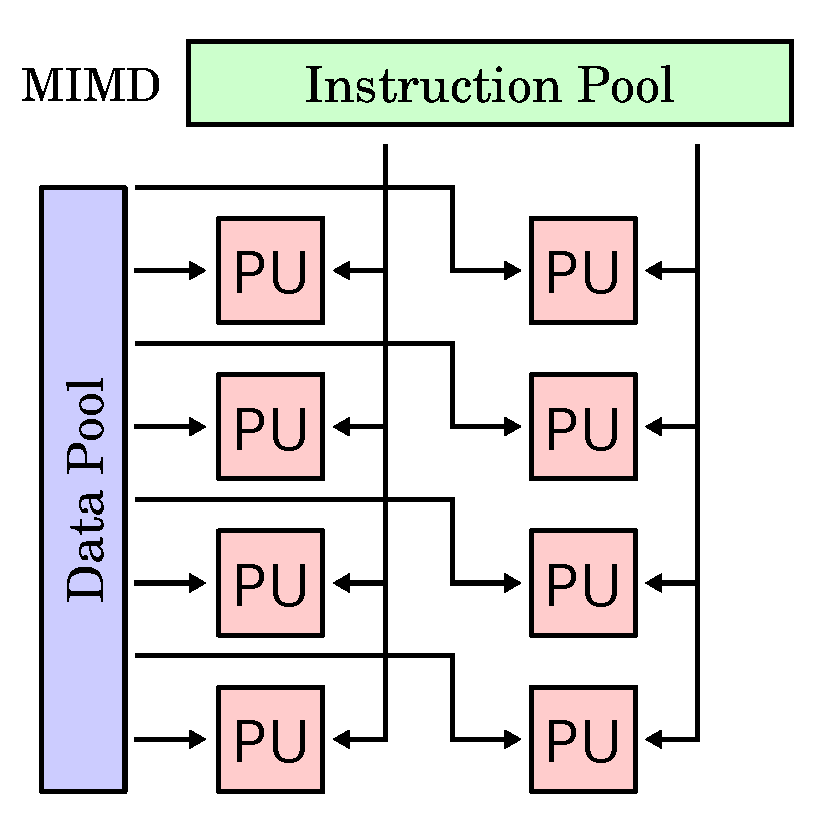
\includegraphics[width=\textwidth/2]{fig/mimd-block-diagram.pdf}
    \label{figure:mimd-block-diagram}
    \caption[
    Block-level overview of a MIMD computer with a shared memory model
    ]{
    Block-level overview of a MIMD computer with a shared memory model.
   http://en.wikipedia.org/wiki/File:MIMD.svg 
   }
\end{center}
\end{figure}


MIMD architecture forms the basis in the great majority all today’s multi-core super scalar processors.
This is in contrast to the early uniprocessors, which were based on SISD, or Single Instruction stream, Single Data stream. 


Examples of well-known MIMD computing platforms today include Intel's Larrabee platform, and computer clusters connected for instance over the internet.

\section{Genetic Algorithms}
\label{ga-algorithms}

Searching is a well known problem in computer science, because it can be used to solve many other problems.
It is possible to search through a collection of solutions to a problem, rather than finding the correct one by traditional means.
This collection is known as the \Gls{search space}.
It is generally easier to verify that a given solution to a hard problem is correct than finding the solution.
A heuristic search tries to make the search more intelligent than looking at each parameter and comparing it to the other.

A genetic algorithm is a specific type of heuristic search algorithm that is very useful for finding approximate solutions for hard optimization and search problems.
A hard problem in this context is a problem for which there exists no algorithm for feasibly computing a solution within a reasonable amount of time.
In practice, this typically means NP-hard problems.
Classical examples of hard problems for which genetic algorithms can find suitable approximations include the Satisfiability Problem, the Traveling Salesman Problem and the Binary Knapsack Problem, to name a few.
Efficiently finding good approximations to this class of problems is extremely important for many heavy industry processes such as planning and scheduling of processes, finding optimal placement and routing of components in microchip manufacturing, and many other business-critical tasks.


The distinguishing feature of a genetic algorithm compared to other heuristic search algorithms is how it performs its search: it mimics the natural process of evolution to find fit approximations within the search space.
A genetic algorithm represents possible solutions to a given problem as individuals of a population.
The individuals' fitness is calculated by a problem-specific fitness function, and fit individuals are combined together to create new individuals, mimicking the process of natural selection.
The idea is that after simulating a number of virtual generations of individuals, the fittest individual will have survived, and provides a good approximation to the solution.

\subsection{Concepts and Definitions}

To fully understand the inner workings of the \Gls{barricelli}, it is useful to become acquainted with the basic concepts of genetic algorithms.
This subsection of the document defines some genetic algorithm concepts that are used elsewhere in the report.

\paragraph{Experiment}
An attempt at solving a problem using a genetic algorithm.

\paragraph{Individual}
One possible solution (good or bad) to a given problem.

\paragraph{Population}
The group of individuals in a given experiment.

\paragraph{Fitness}
An evaluation of how close an individual is to the theoretically perfect individual.
It is calculated by an objective rating function.

\paragraph{Selection}
Probabilistic selection of rated individuals allowed to reproduce.
The probability of picking a certain individual is typically proportional to its fitness rating.

\paragraph{Crossover}
The combination of individuals (parents) in some way to form a new individual (child).
Also called reproduction.

\paragraph{Mutation}
Mutation of an individual.
It is either random or based on problem-specific rules. 

\subsection{Pseudo-code for a General Genetic Algorithm}

Algorithm \vref{algorithm:pseudo-code-for-ga} shows example pseudo code for a general genetic algorithm.

\begin{figure}[H]
\begin{algorithm}[H]
\SetAlgoLined
\DontPrintSemicolon
\KwData{A population of random individuals}
\KwResult{A quite fit individual}
\Begin{
    $ k \longleftarrow 0 $\;
    $ P_k \longleftarrow $ a population of $ n $ randomly-generated individuals\;
    Compute $fitness(i)$ for each $ i \in P_k $\;
    \While{$ max(fitness(i), i \in P_k) <  threshold $ AND $k < maxIterations $}{
        Selection:\;
        Select $ (1 - x_i) \times n $ members of $ P_k $ and insert them into $ P_{k + 1} $\;

        Crossover:\;
	Select $ x_i \times n $ members of $ P_k $, pair them up, produce offspring, insert offspring into $ P_{k+1} $\;


        Mutation:\;
        Mutate $ \mu \times n $ members of $ P_{k + 1} $\;
	Compute $ fitness(i) $ for each $ i \in P_{k+1} $\;
        $k \longleftarrow k + 1 $
    }
    \Return{the fittest individual in $ P_k $}
}
\caption{Generic genetic algorithm}
\label{algorithm:pseudo-code-for-ga}
\end{algorithm}
\end{figure}


\subsection{Generational Genetic Algorithms} \label{background:generational_genetic_algorithms}
Traditionally, genetic algorithms are implemented with discrete generations \cite{hromkovic}
This means that after a loop in the genetic algorithm, a completely new generation has been created by crossover and mutation.
The original population is replaced with the new one, and the algorithm continues only with the new population.

Generational genetic algorithms can be seen as performing these steps:


\begin{enumerate}
    \item Start with an initial population
    \item Calculate the fitness of each individual in the generation
    \item Selection
    \item Crossover
    \item Mutation  
    \item Loop back to step 2 with a newly created population.
\end{enumerate}

The initial population is normally made from randomly generated individuals.
The diversity ensures that it is possible for the generation to evolve towards a solution without getting stuck in an early local maxima.
In the next stage the fitness of each individual calculated, which is very specific for the problem at hand.
If this fitness values exceeds some specified threshold, the solution is deemed good enough and the algorithm stops.
Note that it will not always find a perfect solution, but one that is sufficient for the problem at hand.
If however none of the individuals end up with a fitness value above the threshold, the algorithm continues.

The solution is found during several phases though a selection, crossover and a mutation phase. 
These phases are used to evolve the population through several generations until an appropriate solution is found. 

The selection step aims to choose individuals for reproduction based on their fitness score, meaning that a higher score gives a higher propability of being chosen.
However, this does not necessary mean that only the fittest individuals are allowed to reproduce.
An important concept of the genetic algorithm is to achieve diversity while exploring the different solutions.
Diversity is important to prevent the algorithm from reaching what is known as a local maximum, a result that has a comparative high fitness score for the immediate region in the \gls{search space}.

A sort of evolutionary dead-end, a stage where the solution found is far from optimal but discovering a more optimal one would require several generations of devolving (selecting individuals with non-max fitness from the current population's descendents).

The crossover core uses the individuals from the selection to cross the individuals to produce new individuals.
Because of the initial diversity in the initial population, this will cause the diversity to be large in the beginning.
However they will eventually converge.
The goal of the crossover phase is to converge against a solution by continuously creating a better generation of individuals.
There are several methods for achieving the crossover of individuals, however, the different methods will not be discussed in great detail here.
The different algorithms are highly dependent on the task at hand.
However, the different crossover methods implemented in the employed in the Galapagos architecture will be discussed in greater detail in section \vref{fpga:subsection:genetic_pipeline}.

As a precaution, the individuals are passed through yet another phase: mutation.
The goal of the mutation is to ensure diversity by randomly mutating the individuals by some probability.
The mutation process is usually a simple one that just modifies some of the bits in the individual.
As with the crossover method, algorithms also exist for performing the mutation.


Lastly, it is important to mention that there exists a lot of different classes of genetic algorithms.
They usually employ many different techniques for performing selection, crossover and mutation.
The point of this project is not covering all of them.
In fact, only a subset of problems will be supported on Galapagos architecture.



\subsection{Steady State Genetic Algorithms}
Steady state genetic algorithms do away with the concept of discrete generations.
Rather they continuously select a few individuals, process and return them (or their offspring) to the population.
Older members of the population eventually disappear, based on some selection scheme, preventing the population from growing infinitely large.
This erases the generational border, and has been shown to converge faster towards an optimal solution.
More specifically it allows the algorithm a possible way to work on both rated and unrated individuals at the same time.\cite{steady-state}
This approach is more suited for MIMD architectures, such as the architecture demonstrated in this project.

As steady state algorithms are faster and fitting for MIMD, it was chosen as the main algorithmic goal for the project.




\part{Design and Implementation}

\chapter{System Overview}
    \todo{image of the finished computer}

\section{Application}

The Barricelli computer, which is pictured in Figure \todo{reference image of the finished computer} is a computer designed for solving problems using genetic algorithms.
It is highly optimized for problems for which it is possible to express individuals in 64 bits or less.
The Barricelli can be controlled through one of its external communication channels, such as USB, but can also be commandeered through the built-in buttons and LEDs.

\todo{more}

\section{System Architecture}

This section aims to provide a bird's-eye view of the system architecture of the \Gls{barricelli} computer.

\begin{figure}[H]
\includegraphics[width=\textwidth]{dmpro/Sketch 1 - System Overview.png}
\caption{System Overview}
\label{figure:system-overview}
\end{figure}
\todo{increase font size in illustration}

The requirements in section \vref{section:requirements} state that the \Gls{barricelli} should use an \gls{FPGA} and a microcontroller as system components.
The \Gls{barricelli}'s specialized CPU design is implemented and compiled onto an \gls{FPGA}, and a microcontroller is used to facilitate Input/Output, control and communications between the \gls{FPGA} and the outside world.
A graphical overview illustrating the system architecture can be found in figure \vref{figure:system-overview}.

\section{Components}

This section contains a list of the components in figure \vref{figure:system-overview}, documenting their roles in the system architecture.

\subsection{\gls{FPGA}}

The \gls{FPGA} is a Xilinx Spartan6 LX45\cn Field-Programmable Gate Array, which is a microchip that can be programmed to behave like any arbitrary intergrated circuit.
The \gls{FPGA} is programmed to contain an implementation of the custom \Gls{galapagos} Processor Architecture designed for the \Gls{barricelli} computer.
It is connected to the \gls{SCU} by a 41-bit wide bus, though which the processor can be programmed by users.
The \gls{FPGA} is connected to its own external \gls{SRAM} memory.

\subsection{\gls{SCU}}

The \gls{SCU}, or System Control Unit, is an Energy Micro EFM32GG390F1024-BGA112 microcontroller which administrates communication between the \gls{FPGA} and the outside world.
It is the \gls{SCU}'s job to react to user input, to program the custom processor implemented on the \gls{FPGA} and to perform other administrative duties.
Having a separate microcontroller to perform these tasks minimizes the complexity of the design implemented on the \gls{FPGA}, which means that more resources can be used to create a performant and clean custom processor design.

While only one input and one output are strictly needed to meet the functional requirements, multiple different types of input have been added to the design in the name of safety through redundancy.
The different inputs and outputs are listed in the following subsections.

\subsubsection{USB}

Universal Serial Bus is a bus interface used to facilitate the communication between Barricelli and a host computer.
USB support has become very widespread, to the point where it is difficult to find a computer without several USB ports, and was a natural choice for a main communication link.
Another important reason for choosing USB was because of the large number of software libraries and examples available.

\subsubsection{TIA-232}

TIA-232, more commonly known as RS-232, is a set of standards defining communication over what is commonly known as serial ports.
The serial link is an old standard and a comparatively slow way to transfer data, so it is mainly included as a fallback in case the USB link should fail.

\subsubsection{SD}

Secure Digital (SD) is a memory-card format chosen as a secondary backup as communications channel between the developers and the microcontroller.
Should both the USB and serial ports fail, an SD card could be loaded with the desired instruction and data memory and be read by the microcontroller as if it was a bus.

\subsubsection{LEDs}

The simplest way to get output from the microcontroller is to use LEDs, short for Light-Emitting Diode.
There are a total of 16 LEDs which can be used to display status from the IO controller, or simply show that the IO controller is working on something.

\subsubsection{Buttons}

Buttons is the fastest and simplest way of having some form of user input on the board.
The buttons allow the user to interact with the program running on the SCU without requiring some external IO.

\subsection{Memory}

The \Gls{galapagos} CPU is connected to two separate external memories, the instruction memory and the data memory.
This separation means that the \Gls{galapagos} architecture is a Harvard machine.
This design choice was made because it increases the performance of the machine, since instruction memory and data memory and be accessed independently, and in parallel. 

\subsubsection{Instruction Memory}

The Instruction Memory, labeled as ``INST MEM'' in figure \vref{figure:system-overview}, is the memory that holds the program instructions for the processing units in the \Gls{barricelli} running on the \gls{FPGA}.
The memory is read-only for the processors in the \gls{FPGA}, but can be written to by the \gls{SCU}.
The instruction memory is shared by all the processing units in the \gls{FPGA}.

\subsubsection{Data Memory}

The Data Memory, labeled as ``DATA MEM'' in figure \vref{figure:system-overview}, is the memory that holds processing data for the processors in the \gls{FPGA}.
The memory can be read and read by both the processing units in the \gls{FPGA}, and the \gls{SCU}.
The data memory is shared by all the processing units in the \gls{FPGA}.


\chapter{Processor Design}
	The Barricelli computer features a custom processor design.
The processor is a MIMD processor designed for high performance genetic algorithms computing.
This chapter describes the processor architecture and documents the design decisions made.

\section {Initial requirement}
    \section {Initial requirement}
The assignment require the development of MIMD CPU architecture.
One of the core requirement is to be able to run multiple instruction streams working on multiple data streams.
 \label{fpga:section:initial_requirements}
\subsection{Parallelism}

The Barricelli is a MIMD computer, which means that it can execute multiple different instruction streams on multiple different data streams simultaneously, in parallel.
The cores in the archtecture have each their own program counters and may load different data independantly of each other.
Several of the cores share the same data and instruction memory, however, which makes the Barricelli a shared memory model MIMD computer.



\section{Instruction Set Architecture} \label{fpga:isa:s:isa}
    The \Gls{galapagos} Instruction Set Architecture is the instruction set archtecture designed for the \Gls{barricelli} computer for this project.
The architecture is loosely based on the well-known and tested \gls{MIPS} architecture, but borrows inspiration from many other different sources as well.
Especially inspirational for the design of the \Gls{galapagos} ISA have been the \gls{MIPS} core design principles, which can be found in table \vref{fpga:tbl:mips-design-principles}.

\begin{table}[H]
\centering
    \begin{tabular}{l l} 
     \textbf{Design principle 1} & Simplicity favours regularity.~\cite[p.~79]{compOrgDes}. \\
     \textbf{Design principle 2} & Smaller is faster.~\cite[p.~81]{compOrgDes} \\
     \textbf{Design principle 3} & Make the common case fast.~\cite[p.~86]{compOrgDes} \\
    \hline
\end{tabular}
    \caption{MIPS Design Principles}
    \label{fpga:tbl:mips-design-principles}
\end{table}

The Galapagos ISA was designed and fully specified quite early in the project, which made it an important resource for the rest of the component design process.

While the ISA is thoroughly documented in appendix \vref{appendix:isa}, the rest of this section will present a short overview for the reader's convenience.

\bigskip
\bigskip

The \Gls{galapagos} instruction set architecture is a RISC architecture.
The instructions are kept simple, and only perform very specific and small tasks.
That is, the instructions are low-level instructions executed directly in hardware without the need for additional decoding in form of microinstructions or the like.

\subsection{Instruction Formats}

As \Gls{MIPS}, \Gls{galapagos}, in true \gls{RISC} fashion, has relatively few instruction formats.
These instruction formats are constructed to be regular, which implies that the different information types contained in an instruction are always located in the same positions, when possible.
This makes the instruction decoding process in the processor much simpler.
This is done in accordance with design principle 1 of table \vref{fpga:tbl:mips-design-principles}.

The three instruction formats used in \Gls{galapagos} are the RRR, RRI and RI formats.
They are named after the types of data they contain.
RRR contains three register addresses.
RRI contains two register addresses and one immediate.
RI contains one register address and a larger immediate.

Every instruction has a set of conditional flags that may be set.
Through these flags, a programmer can decide whether or not an instruction will be executed.
This allows for branchless conditional execution of single instructions.
These conditional signals allow for many clever applications - a \gls{nop} instruction can be implemented as any instruction with the condition set to ``never execute''.
Indeed, even conditional branching is implemented as a branch-less conditional!
For a more detailed docummentation of the \gls{galapagos} instruction set architecture, the reader is encouraged to read appendix \vref{appendix:isa}.


\subsection{Genetics Instructions}

One of the requirements in section \vref{section:requirements} was that the ISA should support genetic-specific instructions to facilitate performant genetic algorithms programming.
Present in the \Gls{galapagos} ISA are the genetic instructions \texttt{ldg}, \texttt{stg} and \texttt{setg}.
They are the instructions for loading and storing \glspl{individual} to the genetics accelerator, and configuring the genetics accelerator, respectively.
With these instructions available to the programmer, using the genetics accelerator is easy and painless.
The reader may refer to the ISA documentation in appendix \vref{appendix:isa} for in-depth documentation about how the genetics instructions are used.



\section {Processor Architecture}
    \begin{figure}[H]
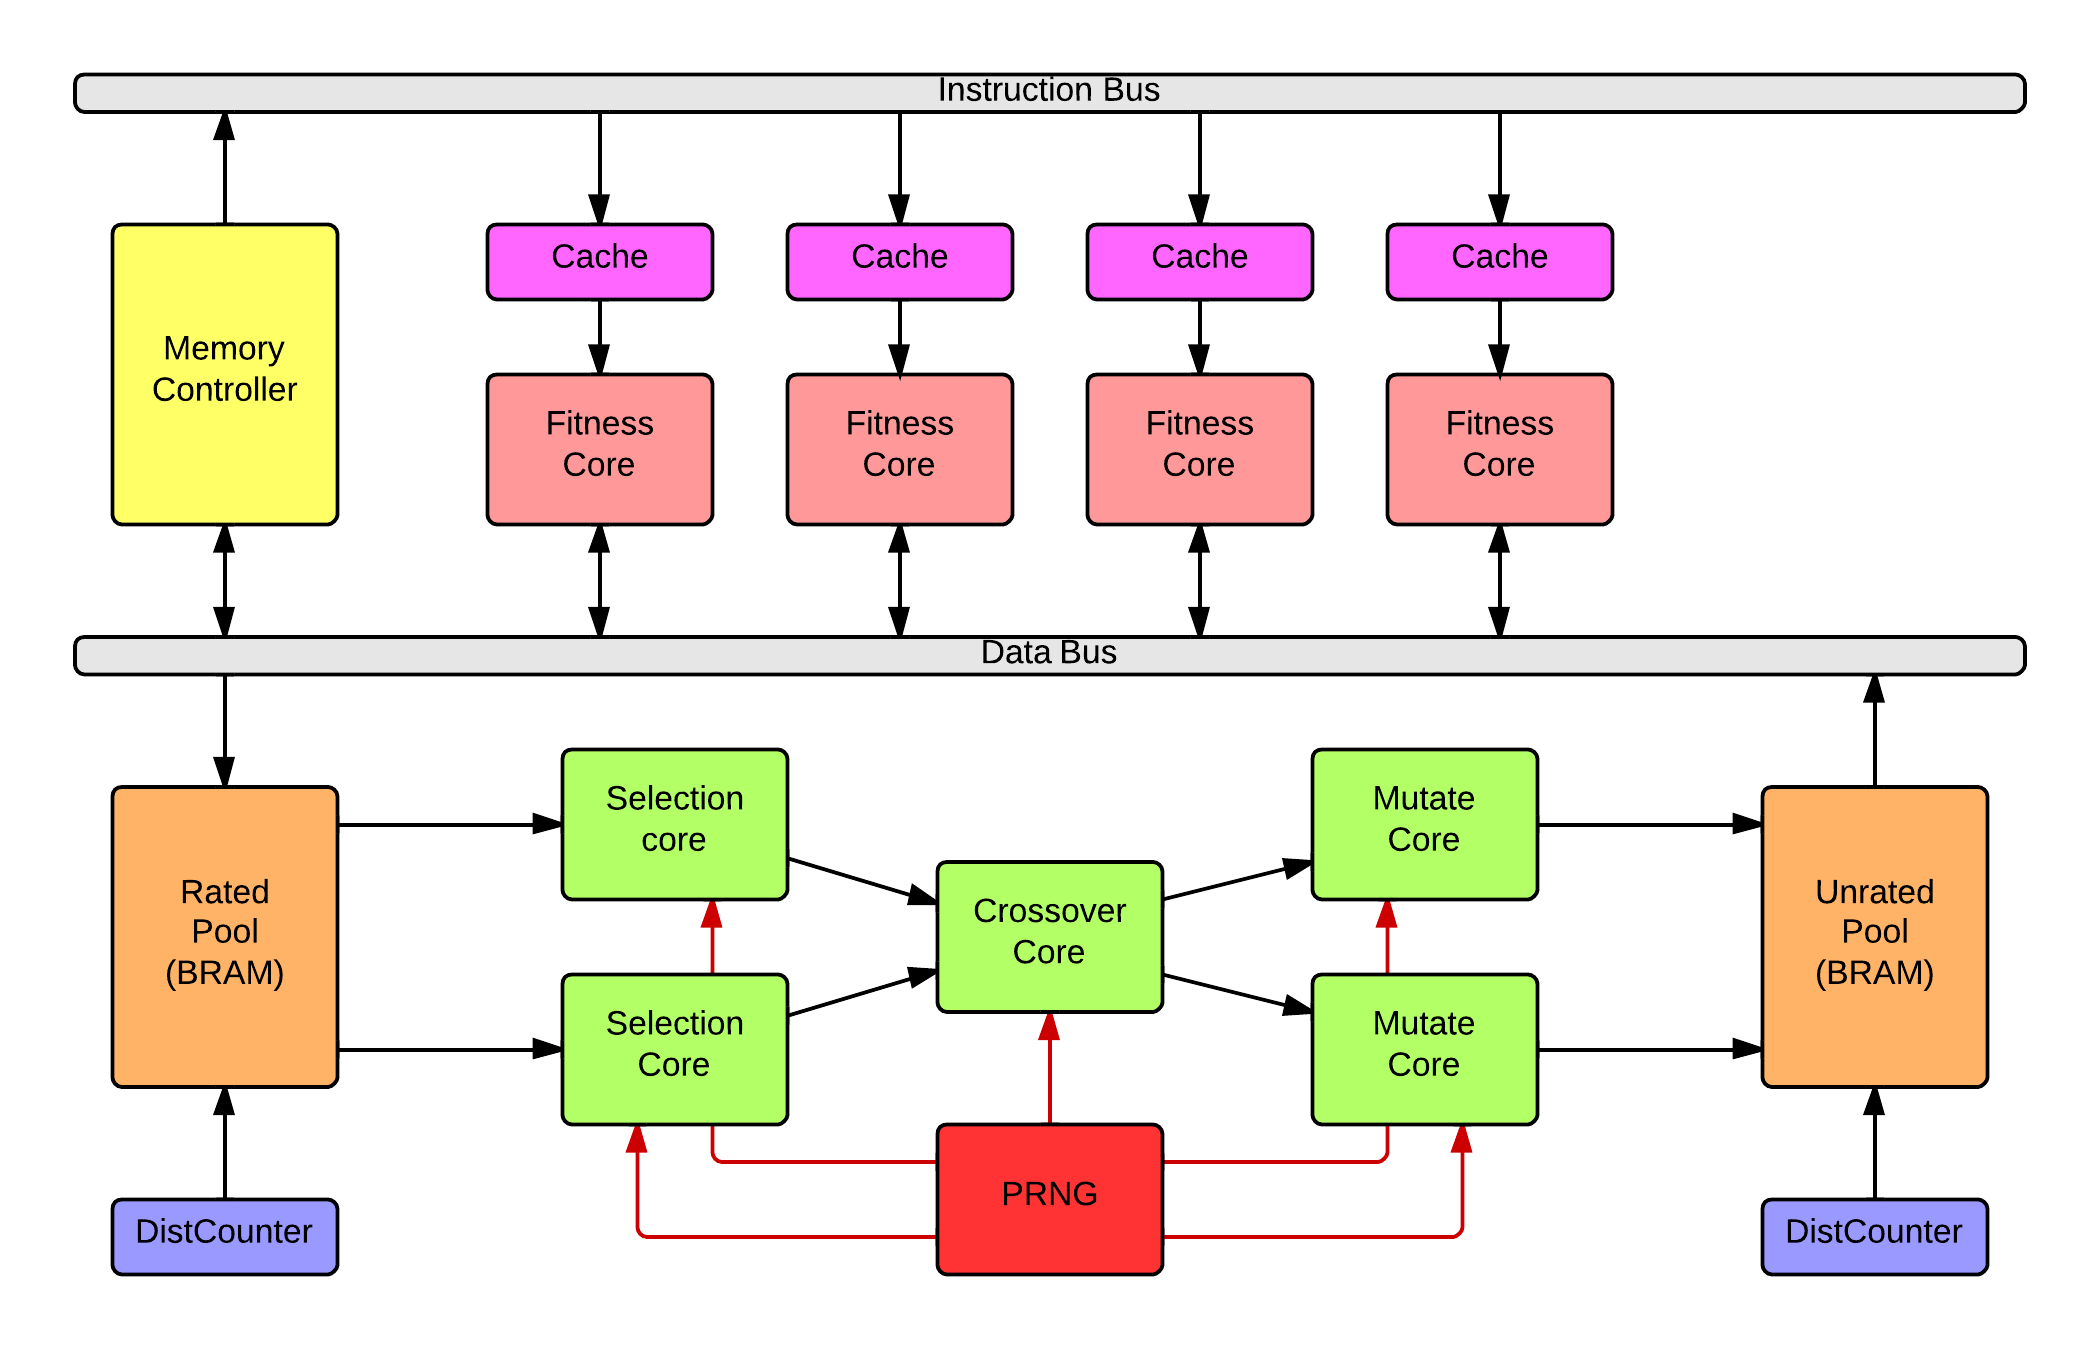
\includegraphics[width=\textwidth]{fpga/fig/processor_architecture.png}
\caption{The figure shows the final processor architecture. Most of the figures seen in this picture as for instance "fitness core", are abstractions of more complex logic at lower levels (mostly MSI and LSI components). }
\label{figure:fpga-architecture}
\end{figure}

\todo{Modify figure \vref{figure:fpga-architecture} so that it is easy to see that the number of fitness cores is configurable.}

The processor architecture designed for the Barricelli computer is a very clean design, and the key to its high performance lies in its simplicity.
The architecture contains a number of general cores, which in this context are named fitness cores.
The fitness cores are general purpose cores in the sense that they are programmable and turing complete, but for genetic algorithm applications the cores are intended to calculate fitness scores of individuals.

The number of fitness cores is configurable.
The reference implementation of the Barricelli computer is configured to have 7 fitness cores.

Common genetic algorithms operations are performed by a separate hardware accelerator pipeline.
This accelerator consists of several operation-specific special cores for selection, crossover and mutation.
The fitness cores and the genetic pipeline are all connected to a single data bus.
To avoid any memory synchronization issues the data bus is controlled by a central arbitration unit.

The processor architecture is illustrated in figure \vref{figure:fpga-architecture}.


\subsection{Instruction Memory}
\label{subsec:fpga-instruction-memory}
The \Gls{barricelli} is a \Gls{harvard machine}.
The memory is split into instruction and data memory.
This is done to achieve better memory throughput, because both memories can be accessed simultaneously.
The instruction memory is organized in a two layer memory hierarchy, with slower external memory (\gls{SRAM}) and faster, internal on-chip caches (\gls{BRAM}).
This separation combines the high instruction thoughput of fast on-board memory wit the comfortably spaceous data storage capabilities of a larger, slower chip external chip.

Each fitness core has its own private instruction memory cache which buffers instructions to decrease the number of slow memory accesses needed during runtime.
Access to an instruction cache is handled by a fitness core's dedicated cache controller, which is responsible for locating and transferring instructions from the instruction memory.
In case of a cache miss, the data-requesting core is halted until the instruction is transferred from memory.
A pseudo-algorithm describing the cache fetch operation can be found in algorithm \vref{algorithm:cache-operation}.
This scheme is created to resolve the conflicts that arise from using shared memory. 

\begin{algorithm}[H]
\SetAlgoLined
\DontPrintSemicolon
\KwData{ $ a = $ an instruction address \newline
$ Ci = $ an array of instructions \newline
$ Ca = $ an array of the corresponding addresses \newline
$ M = $ the instruction memory, indexable by instruction addresses
}
\KwResult{The instruction at address $ a $}
\Begin{
    \If{$ a = Ca[A \bmod{512}] $}{
        \Return{$ Ci[A \bmod{512}] $}
    }\Else{
        $ Caa \bmod{512}] \longleftarrow a $\;
        $ Ci[a \bmod{512}] \longleftarrow M[a] $\;
        \Return{$ Ci[A \bmod{512}] $}
    }
}
\caption{Fetching an instruction from the cache}
\label{algorithm:cache-operation}
\end{algorithm}


\subsection{Data Memory}
\label{subsec:fpga-data-memory}
The \gls{galapagos} architecture is a \gls{MIMD} architecture with shared memory.
In the \Gls{barricelli} computer, a central memory controller is responsible for synchronizing memory access on the shared data bus.
Each component that wants to access memory must go through the memory controller, and follow the proper memory access request protocol.
The controller is constructed in a way that only allows one fitness core to be able to carry out a memory request at a single time.
In case of multiple memory requests, the controller performs a selection deciding in which order the requesting cores is granted the bus.
The precise technique of selection can be seen in algorithm \ref{algorithm:round-robin-selection}.
This may introduce a potential bottleneck for memory-bound problems.
For this reason, each fitness core has a generous 31 general purpose registers, which should reduce the data memory load quite a bit.

\begin{figure}[H]
\begin{algorithm}[H]
\SetAlgoLined
\DontPrintSemicolon
\KwData{$ Requests = $ requests signals from the fitness cores\newline 
$ Request = $ 2-bits specifying the operation}
\Begin{
    $ Requests \longleftarrow $ requests from the fitness cores\;
    \While{$ True $}{
        \For {request in Requests} {
            \If{request $=$ asserted}{
                performMemoryOperation()
            }
        }
        
    }
}
\caption{Round-robin selection}
\label{algorithm:round-robin-selection}
\end{algorithm}
\end{figure}


The selection algorithm is based on round-robin scheduling, and will be explained in further detail here.
The request signals of \emph{fitness cores} are checked in turn to check if one of the cores has requested the memory bus.
The type of request is determined by combination of two request signals sent by each \emph{fitness core}.
The signals refer to either a \emph{NOP}, \emph{READ}, or \emph{WRITE} operation.
In case of \emph{NOP}, the algorithm moves on to check the next state request lines.
It continues doing this in this fashion until a \emph{READ} or \emph{WRITE} request is encountered. 

When a \emph{READ} or \emph{WRITE} operation is encountered, the \emph{data controller} starts to carry out the request from the fitness core.
Performing a memory operation takes at least four cycles, as the processor word size is 64 bits, while the memory bus to the external memory chips are only 16 bits wide.
Because of this, data needs to be shuffled across the bus 16-bits at a time, which accounts for the four cycle minimum for data operations.

For the external memory to be operated correctly by the memory controller, the proper control signals need to be set at the correct times. The signals required differs depending on the type of operation, \emph{READ} or \emph{WRITE}. The timing diagrams can be seen in figure \ref{fpga:fig:timing:dmem:read} and \ref{fpga:fig:timing:dmem:write}, respectively. 

\todo{Check text}

\begin{figure}[H]
  \centering
  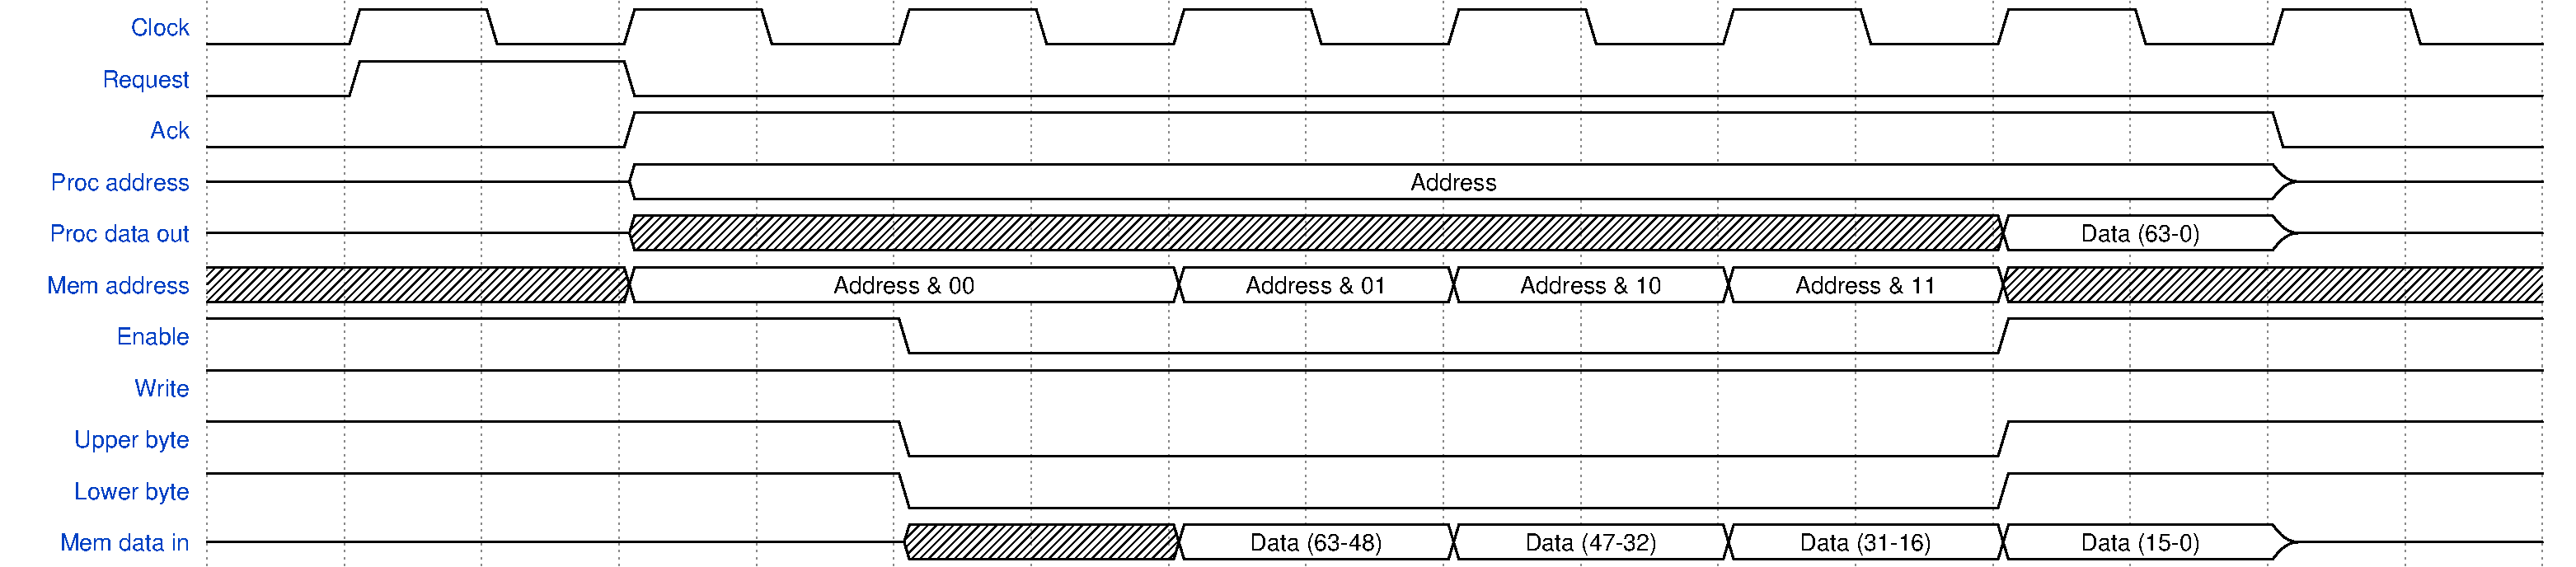
\includegraphics[width=\textwidth]{fpga/fig/timing/data_mem_read.pdf}
  \caption{Data memory read cycle}
  \label{fpga:fig:timing:dmem:read}
\end{figure}

\begin{figure}[H]
  \centering
  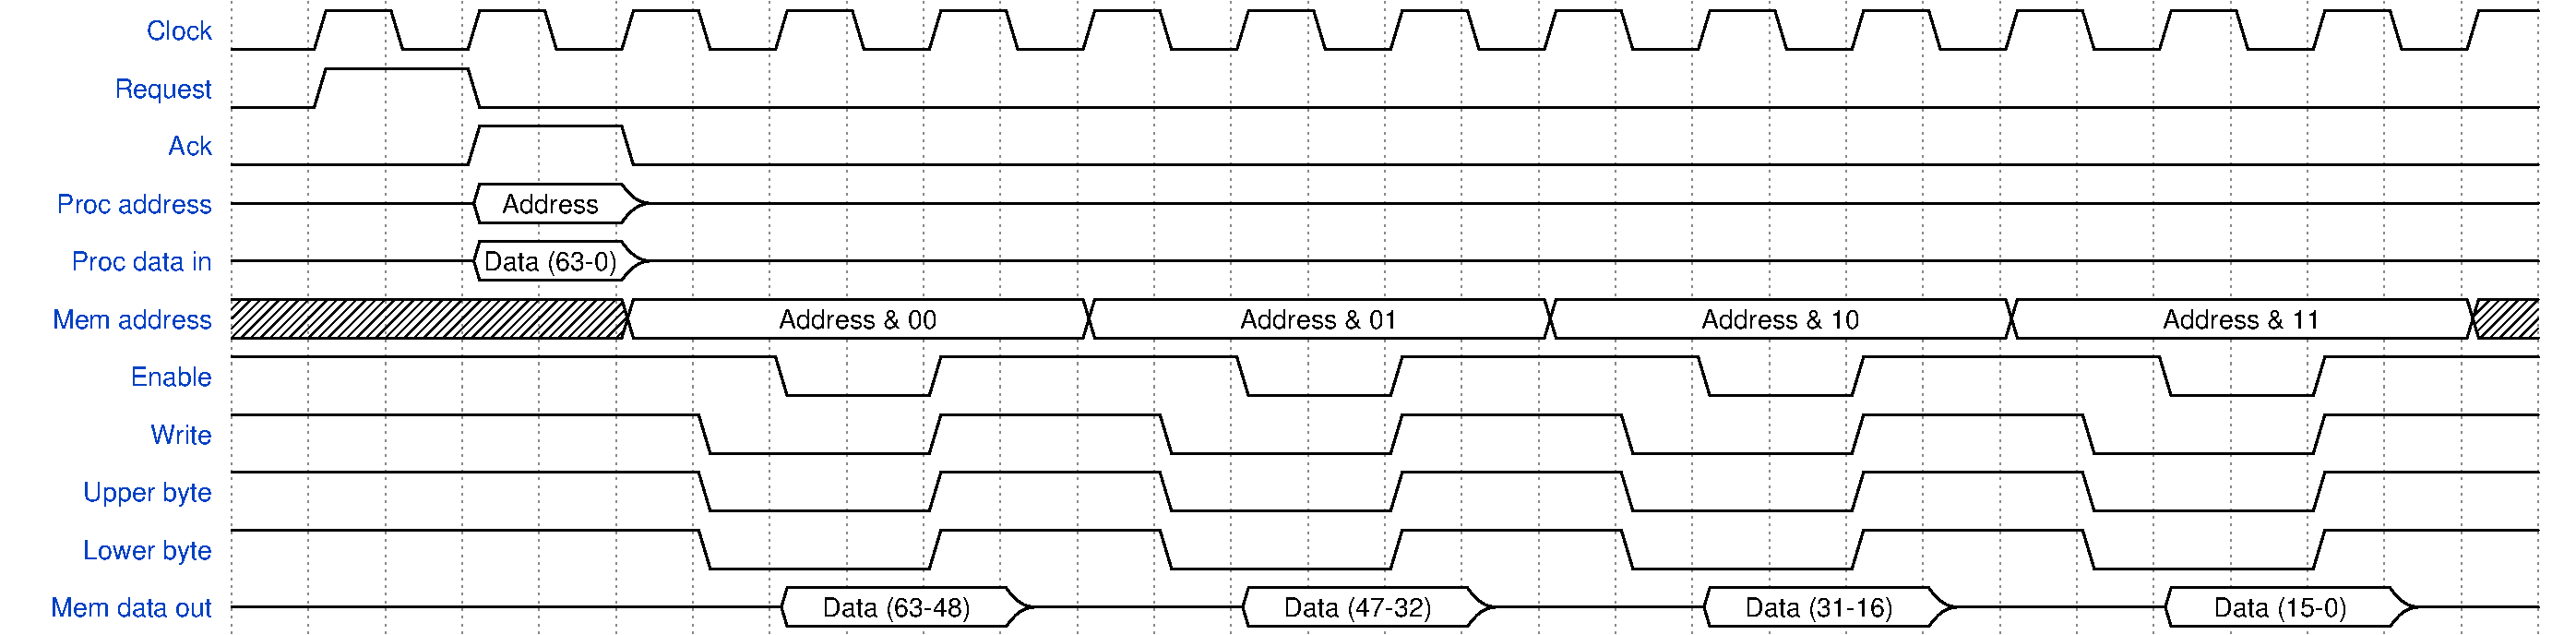
\includegraphics[width=\textwidth]{fpga/fig/timing/data_mem_write.pdf}
  \caption{Data memory write cycle}
  \label{fpga:fig:timing:dmem:write}
\end{figure}

As is immediately apparent in figures \vref{fpga:fig:timing:dmem:read} and \vref{fpga:fig:timing:dmem:write}, the number of cycles required for load and store operations are are 5 and 13 cycles, respectively.
A state machine is implemented in the \emph{data memory controller} to handle interfacing with the external memory chips.
This state machine is responsible for controlling that the different signals are set according to the diagrams.
For more detailed view of the \emph{Data memory controller}, the reader is advised to study the state machine diagram in figure \ref{fpga:fig:mem:data_memory_ctrl_state_machine} and the accompanying data path in figure \ref{fpga:fig:mem:data_memory_ctrl}.

\begin{figure}[H]
  \centering
  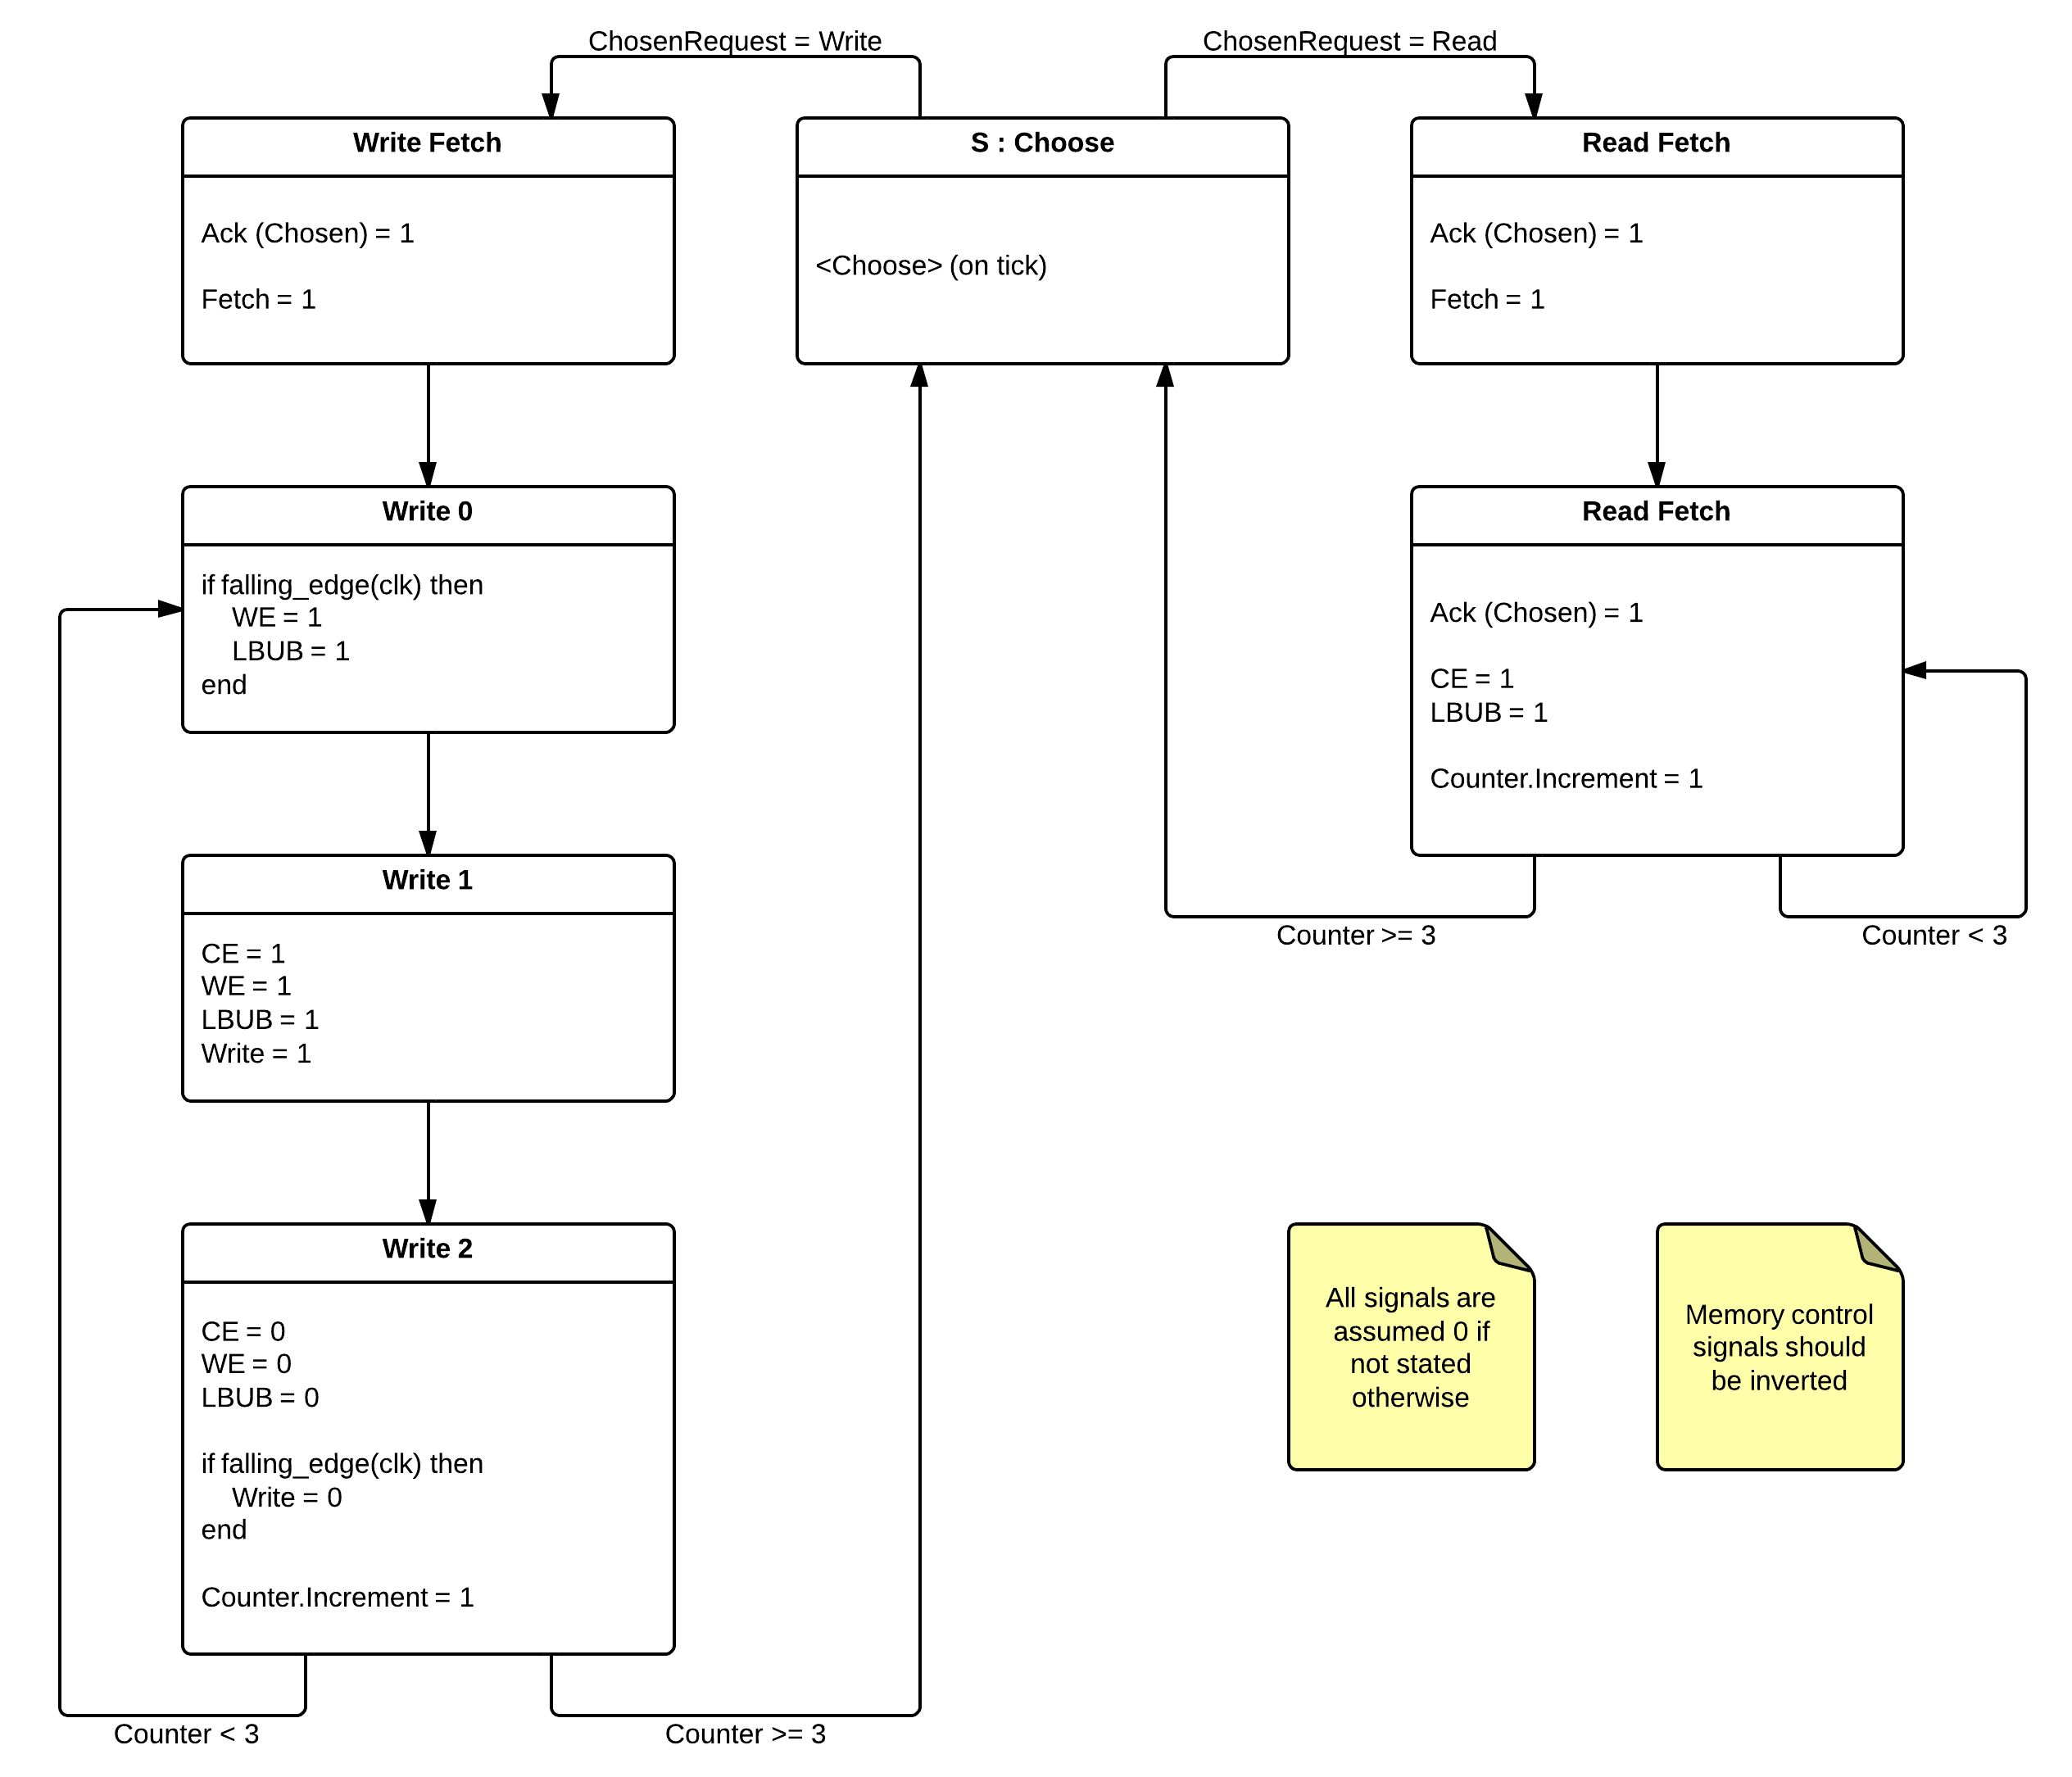
\includegraphics[width=\textwidth]{fpga/fig/memory_ctrl_state_machine.png}
  \caption{Data memory controller state machine}
  \label{fpga:fig:mem:data_memory_ctrl_state_machine}
\end{figure}


\begin{figure}[H]
  \centering
  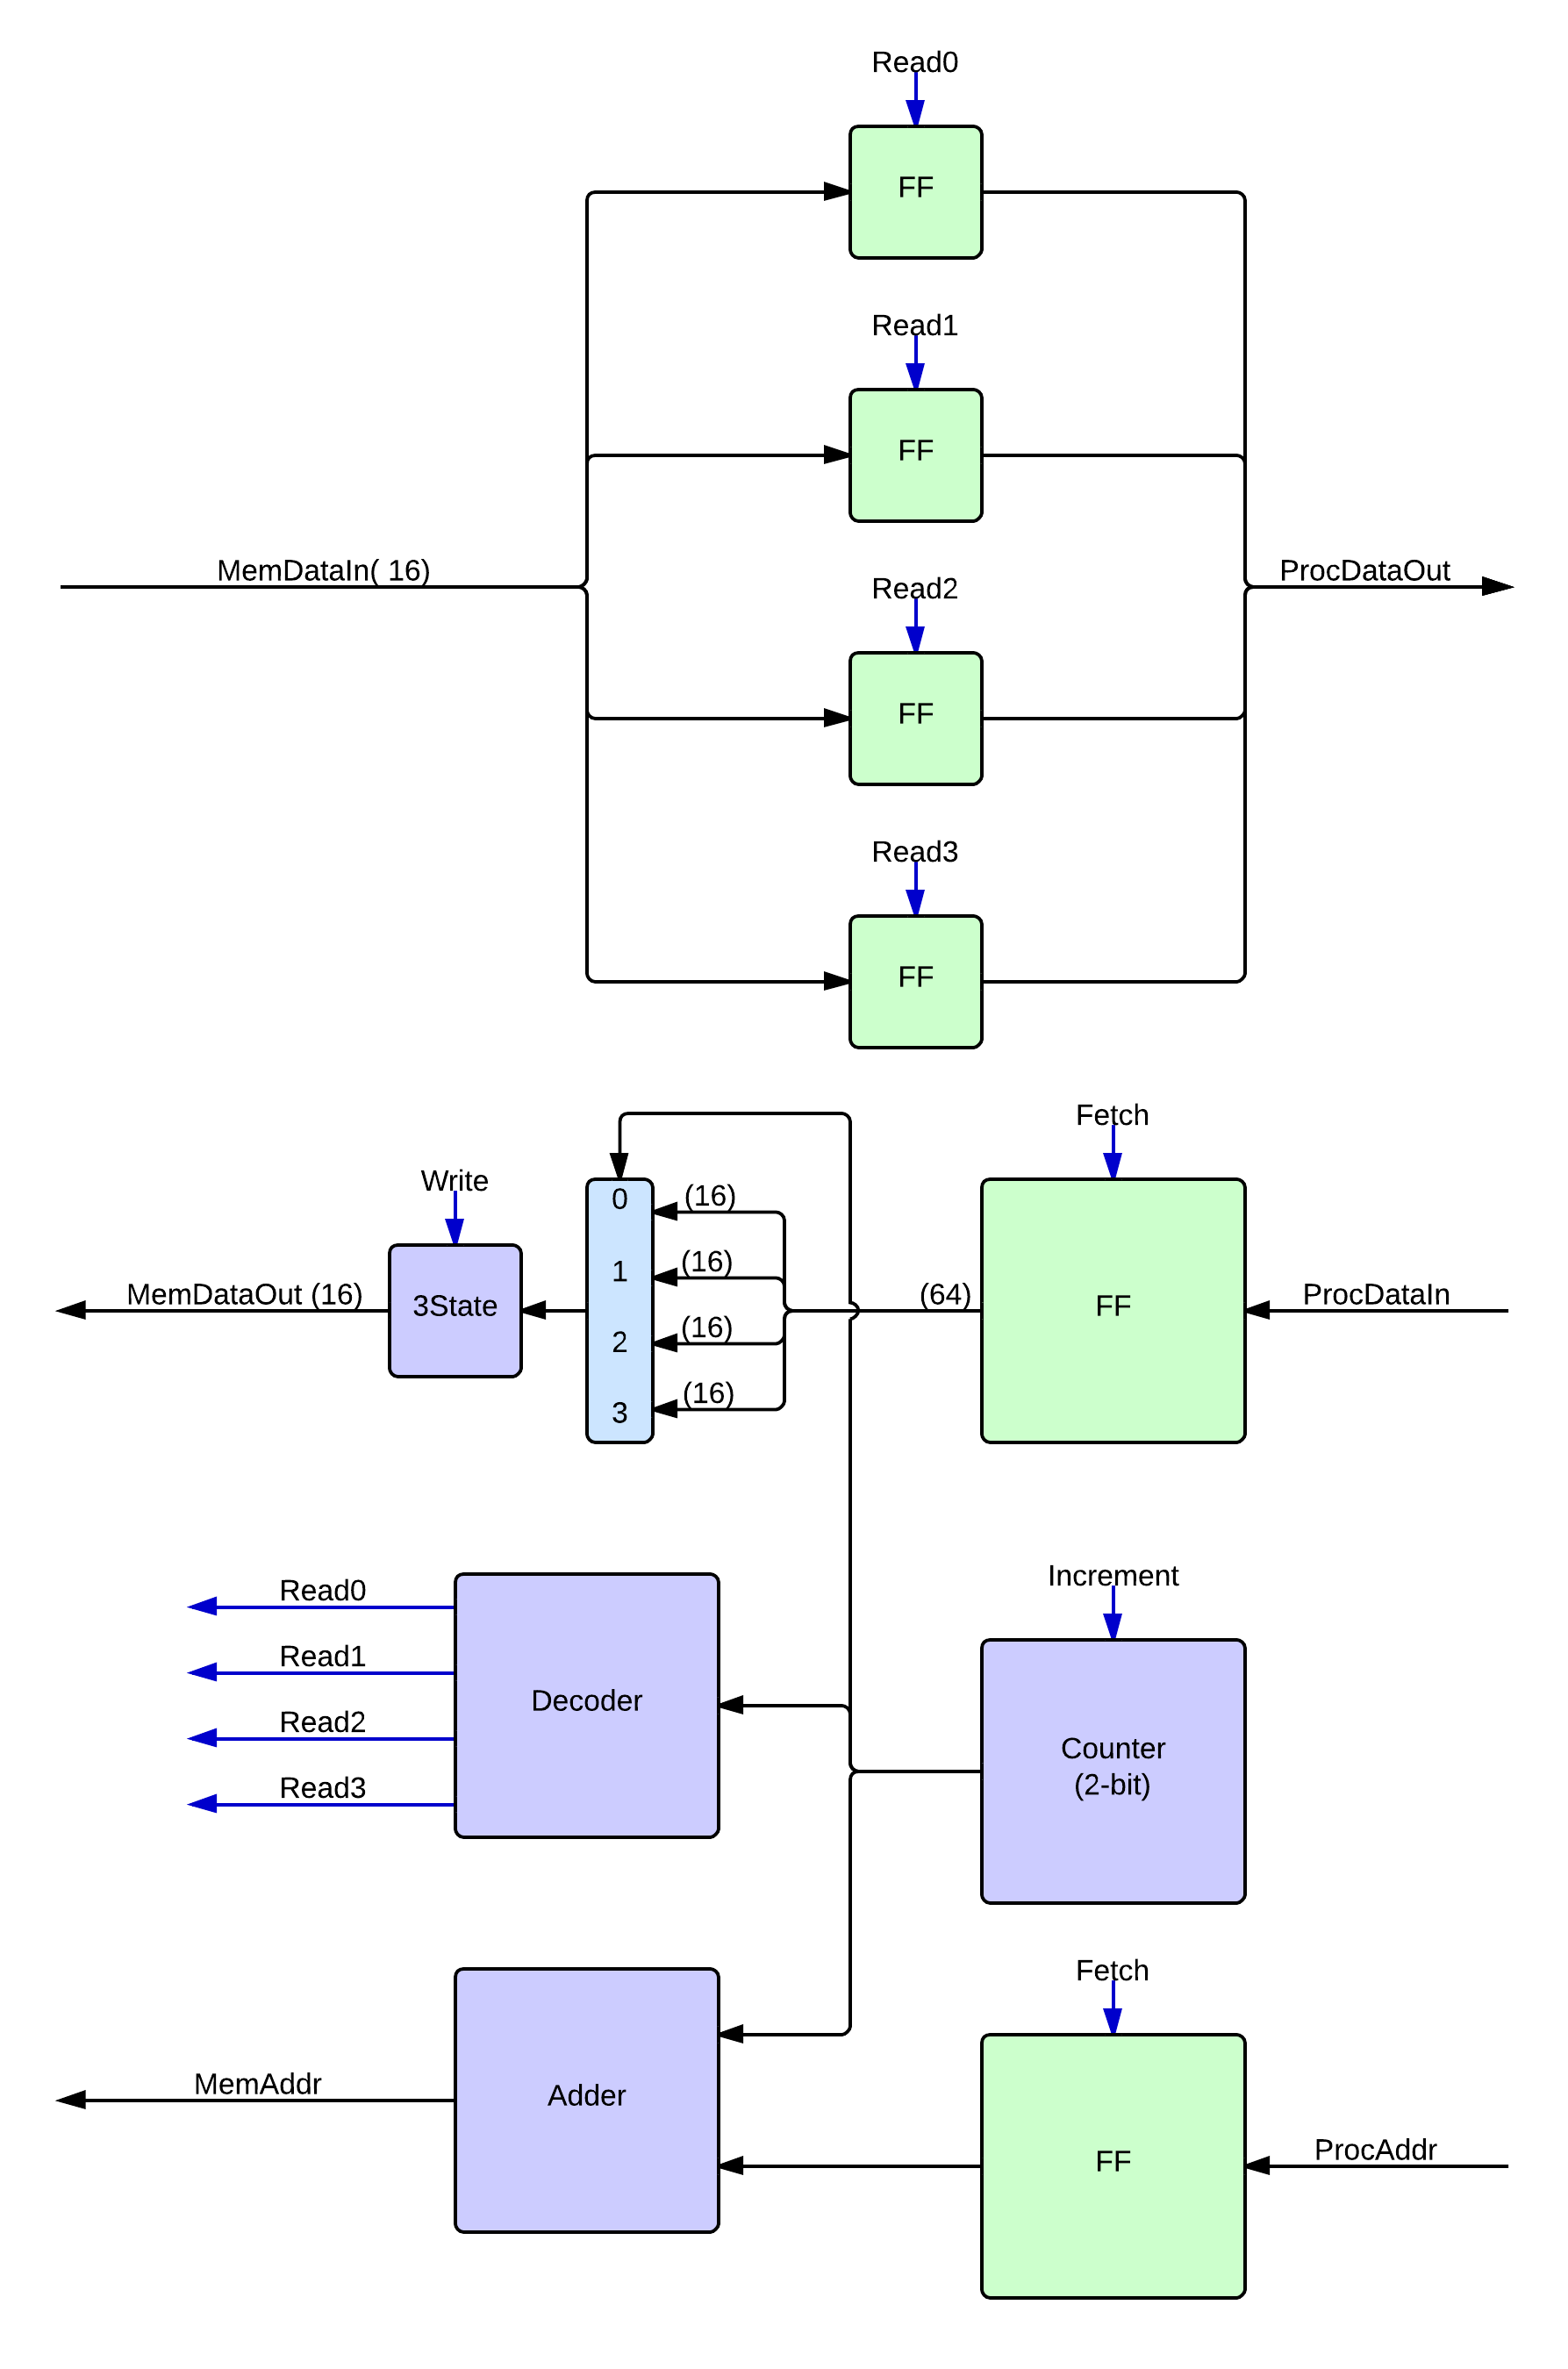
\includegraphics[width=\textwidth]{fpga/fig/memory_ctrl.png}
  \caption{Data memory controller signals mapping}
  \label{fpga:fig:mem:data_memory_ctrl}
\end{figure}


\todo{write about and ref to above graphs}


\subsection{Rated and Unrated Pools}
Individuals making up the populations are stored on the FPGA for for faster access. These are stored in \emph{BRAM} on the FPGA. This implies a lot faster access times, compared to access times to the external memory, as mentioned in (?). This is done to achieve better memory throughput when executing the algorithms. The pools are further divided into two separate \emph{BRAM} blocks, one for rated individuals, and one for un-rated. This is done to achieve even better memory throughput. The increased throughput are achieved because the different computational can work on the rated and un-rated pool simultaneously. For instance while one fitness core is storing a ranked individual, while another fitness core is fetching a new individual for ranking. 

\todo{More details and better explanation} 

Both the rated pool and the unrated pool is associated with the a controller, referred as the \emph{Genetic controller}. As with the data controller, this controller is responsible for granting access for the rated and unrated pool. This buses in question are, however, not the same as those used to access the data memory. The genetic controller use their own separate buses. The controller is based on mostly the same idea as the data controller described in section (?). The when performing genetic operations, the fitness cores need to request the data bus by using two request signals. The combination of these signals refer to the operation the fitness core requests from the genetic controller. 

The genetic cores continuously performs a round-robin in order to grant bus to the requesting fitness core. The logic surrounding the different operations are implemented as an state machine to divide the operations in different clock cycles. This is the same method as used in the data controller.







The state machine can be seen in figure(?)




\subsection{PRNG Module}
The genetic algorithms need diversity in the search space in order to be able to converge to a solution. To achieve this, the architecture need some way of creating sufficiently random numbers. These generated numbers do not need to be true randoms number, this implies that a psudo number generator will suffice. 

    
 

\subsection{Fitness Core} \label{fpga:fitness:ss:design_of_the_fitness_core}
    \subsection{Design of fitness core}

The design of the fitness core is highly influenced by MIPS.
The core is designed as a five stage pipeline.
The goal is to make it as simple as possible, and at the same time harvest efficiency by instruction level parallelism.
The more advanced features like branch prediction and instruction scheduling are not taken into consideration while designing the CPU.
The hazard detection schemes will be made simple.
The hazard resolutions will be made in software as well as in hardware.
The plan is to simply stall when we encounter any hazards in the pipeline.
The assembler will handle the most obvious ones to achieve efficiency, while the hardware will simply stall when hazards are detected.

\fxnote {The hazard scheme may change if time}
 \label{fpga:subsection:fitness_core}


\subsection{The Genetic Pipeline}
\label{fpga:subsection:genetic_pipeline}
\todo{some words about the genetics accelerator}
The galapagos architecture includes a highly specialised pipeline for performing genetic operations. The pipeline is based on the observation that selection, crossover, and mutation works similar for a specific subset of problems. These can therefore be implemented as hardware accelerators constructed for performing one specific task. Constructing such accelerators has been proven to be very beneficial regarding performance. Designing specialised hardware is usually simpler and thereby more effective than constructing general purpose components.\todo{Bullshit ?} This pipeline will effectively relieve the general cores, the fitness cores, from computing the evolution of individuals. The idea is that these will make the fitness cores able to only focus on the computation of fitness ranking, which is considered computational intensive. In the mean time the \emph{genetic pipeline} can produce new data for ranking. These operations could have been performed by the processor, however, the processor is badly suited for these kind of operations. Note that the instructions in the pipeline actually uses 5 cycles in order to complete propagate through the pipeline. It is a far better to only use one cycle in order to complete the one specific operation.  

The genetic pipeline is constructed with three specialised cores for performing selection, crossover, and mutation. These are operations that occurs frequently in genetic algorithms. These are connected to two internal memory banks on the \emph{FPGA}, namely the unrated and rated pool.


-Abstraction for the programmer. Simpler to program.
-Do not need components like ALU
- effective 
- Less control over the genetic pipeline
- 



\subsubsection {Selection Core} \label{fpga:selection:ss:selection_core}
    \input{fpga/selection-core} \label{fpga:subsection:selection_core}

\subsubsection{Crossover Core} \label{fpga:crossover:ss:crossover_core}
    \input{fpga/crossover-core} \label{fpga:subsection:crossover_core}

\subsubsection{Mutation Core}\label{fpga:mutation:ss:mutation_core}
    \input{fpga/mutation-core} \label{fpga:subsection:mutation_core}




\subsection{Parallelism}
\todo{awkwardly placed section.. move it somewhere else?}
The Barricelli is a MIMD computer, which means that it can execute multiple different instruction streams on multiple different data streams simultaneously, in parallel.
The four\cn fitness cores in the archtecture have each their own program counters and may load different data independantly of eachother.
They all share the same data and instruction memory, however, which makes the Barricelli a shared memory model MIMD computer.
Additionally, the genetic pipeline contains multiple specialized cores, which can also execute independant, less general instruction streams on independant data.

 \label{fpga:section:cpu_architecture}


\chapter{PCB}
	All the electronic devices are powered by white smoke. When smoke goes out, device is dead.

― Milan Nikolic



%%Initial requirements
\section {Initial requirement}
The assignment require the development of MIMD CPU architecture.
One of the core requirement is to be able to run multiple instruction streams working on multiple data streams.
 \label{fpga:section:initial_requirements}


The \Gls{galapagos} Instruction Set Architecture is the instruction set archtecture designed for the \Gls{barricelli} computer for this project.
The architecture is loosely based on the well-known and tested \gls{MIPS} architecture, but borrows inspiration from many other different sources as well.
Especially inspirational for the design of the \Gls{galapagos} ISA have been the \gls{MIPS} core design principles, which can be found in table \vref{fpga:tbl:mips-design-principles}.

\begin{table}[H]
\centering
    \begin{tabular}{l l} 
     \textbf{Design principle 1} & Simplicity favours regularity.~\cite[p.~79]{compOrgDes}. \\
     \textbf{Design principle 2} & Smaller is faster.~\cite[p.~81]{compOrgDes} \\
     \textbf{Design principle 3} & Make the common case fast.~\cite[p.~86]{compOrgDes} \\
    \hline
\end{tabular}
    \caption{MIPS Design Principles}
    \label{fpga:tbl:mips-design-principles}
\end{table}

The Galapagos ISA was designed and fully specified quite early in the project, which made it an important resource for the rest of the component design process.

While the ISA is thoroughly documented in appendix \vref{appendix:isa}, the rest of this section will present a short overview for the reader's convenience.

\bigskip
\bigskip

The \Gls{galapagos} instruction set architecture is a RISC architecture.
The instructions are kept simple, and only perform very specific and small tasks.
That is, the instructions are low-level instructions executed directly in hardware without the need for additional decoding in form of microinstructions or the like.

\subsection{Instruction Formats}

As \Gls{MIPS}, \Gls{galapagos}, in true \gls{RISC} fashion, has relatively few instruction formats.
These instruction formats are constructed to be regular, which implies that the different information types contained in an instruction are always located in the same positions, when possible.
This makes the instruction decoding process in the processor much simpler.
This is done in accordance with design principle 1 of table \vref{fpga:tbl:mips-design-principles}.

The three instruction formats used in \Gls{galapagos} are the RRR, RRI and RI formats.
They are named after the types of data they contain.
RRR contains three register addresses.
RRI contains two register addresses and one immediate.
RI contains one register address and a larger immediate.

Every instruction has a set of conditional flags that may be set.
Through these flags, a programmer can decide whether or not an instruction will be executed.
This allows for branchless conditional execution of single instructions.
These conditional signals allow for many clever applications - a \gls{nop} instruction can be implemented as any instruction with the condition set to ``never execute''.
Indeed, even conditional branching is implemented as a branch-less conditional!
For a more detailed docummentation of the \gls{galapagos} instruction set architecture, the reader is encouraged to read appendix \vref{appendix:isa}.


\subsection{Genetics Instructions}

One of the requirements in section \vref{section:requirements} was that the ISA should support genetic-specific instructions to facilitate performant genetic algorithms programming.
Present in the \Gls{galapagos} ISA are the genetic instructions \texttt{ldg}, \texttt{stg} and \texttt{setg}.
They are the instructions for loading and storing \glspl{individual} to the genetics accelerator, and configuring the genetics accelerator, respectively.
With these instructions available to the programmer, using the genetics accelerator is easy and painless.
The reader may refer to the ISA documentation in appendix \vref{appendix:isa} for in-depth documentation about how the genetics instructions are used.



%%Galapagos architecture
\begin{figure}[H]
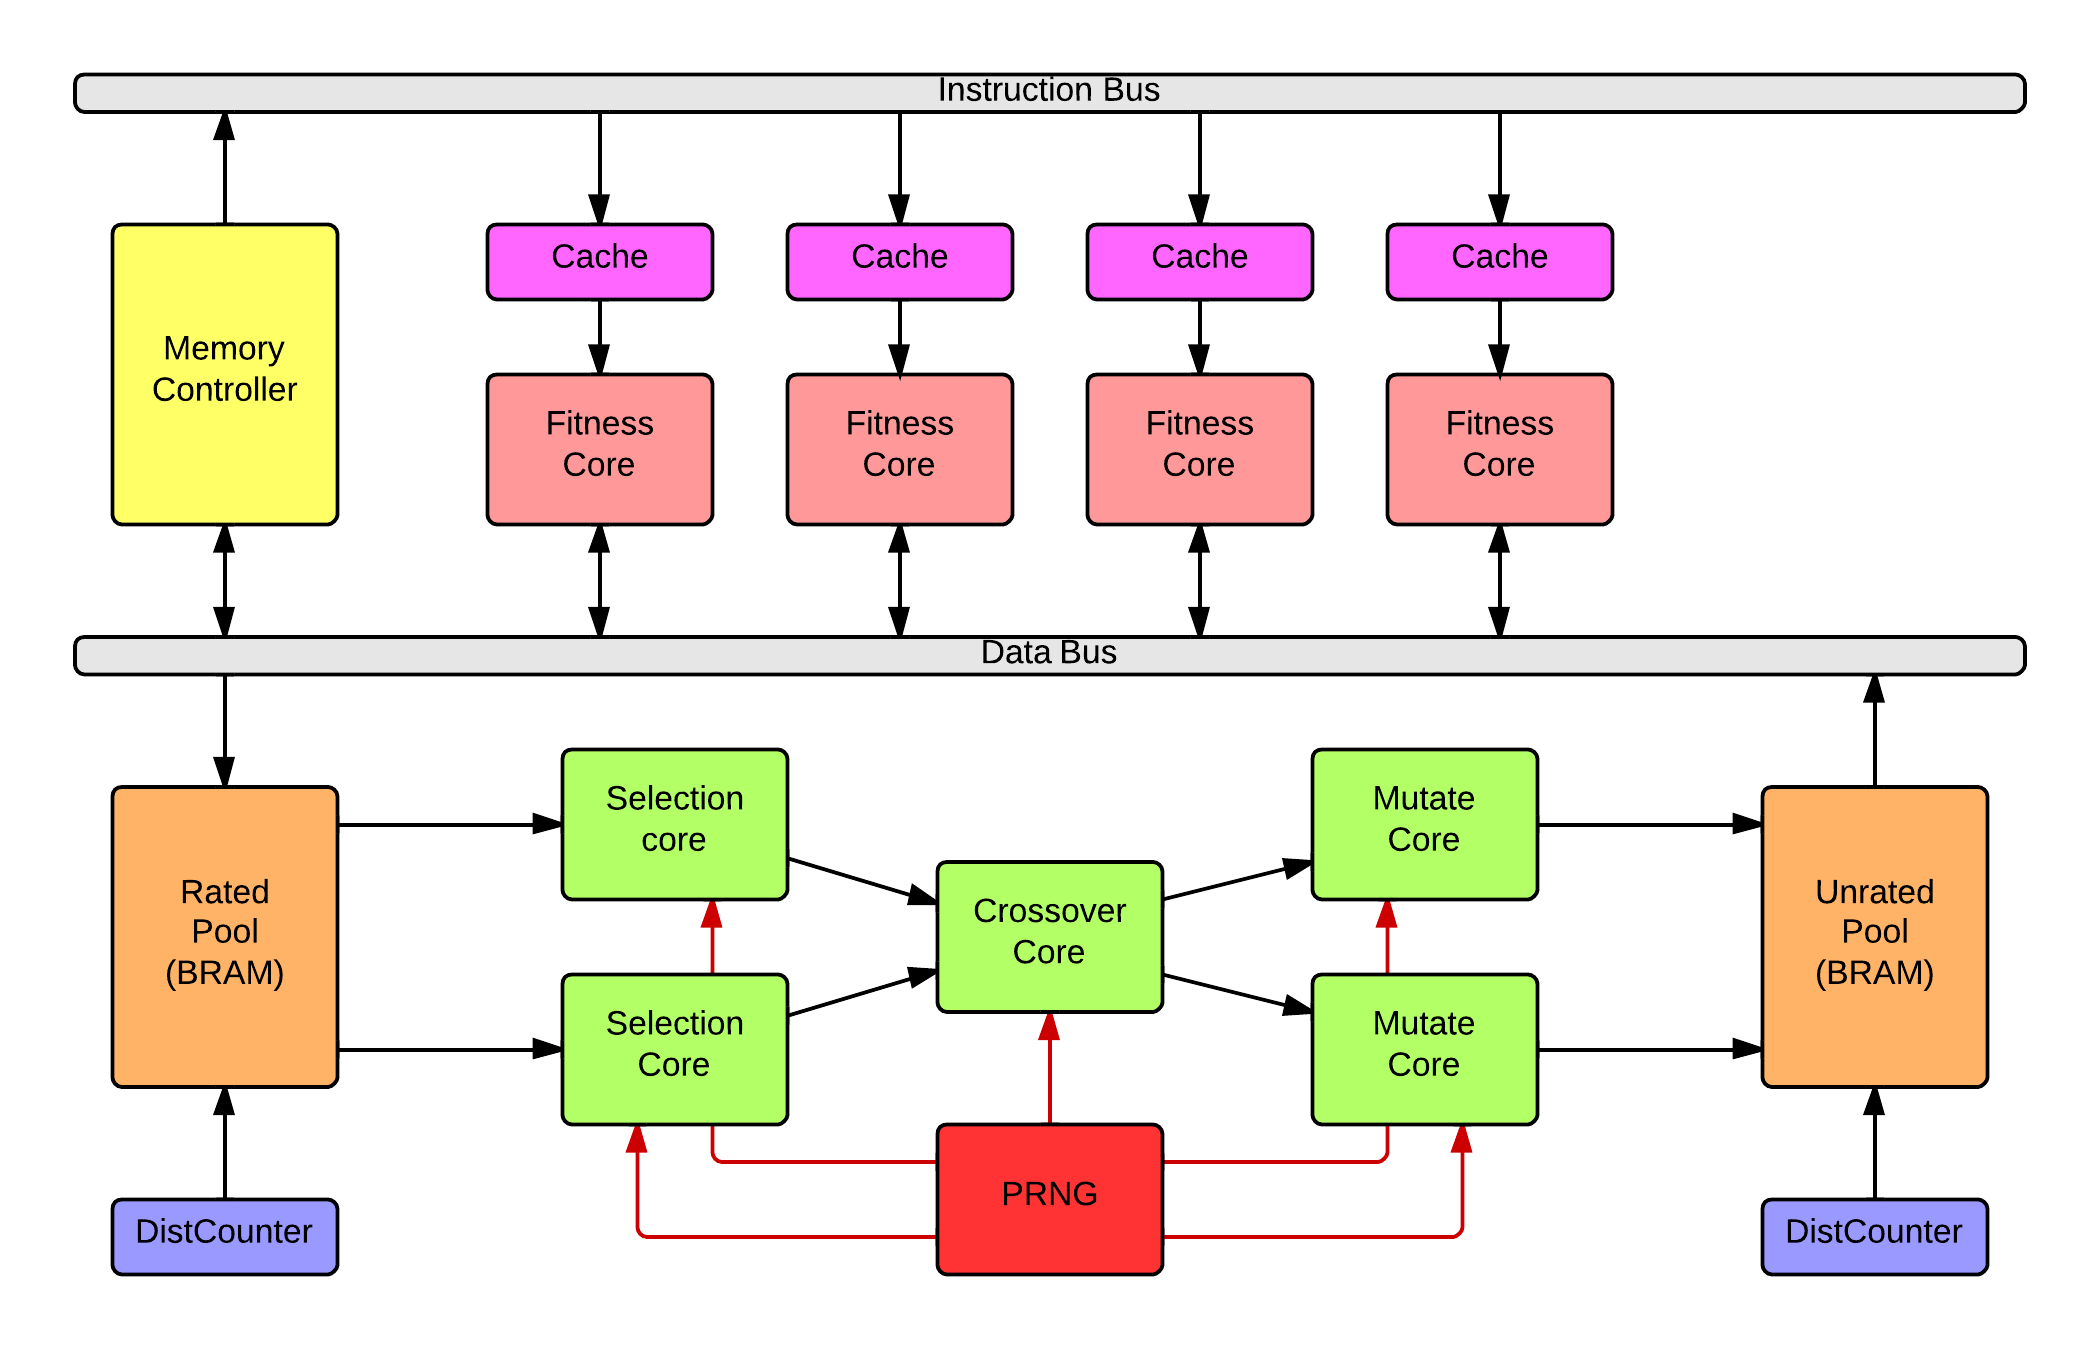
\includegraphics[width=\textwidth]{fpga/fig/processor_architecture.png}
\caption{The figure shows the final processor architecture. Most of the figures seen in this picture as for instance "fitness core", are abstractions of more complex logic at lower levels (mostly MSI and LSI components). }
\label{figure:fpga-architecture}
\end{figure}

\todo{Modify figure \vref{figure:fpga-architecture} so that it is easy to see that the number of fitness cores is configurable.}

The processor architecture designed for the Barricelli computer is a very clean design, and the key to its high performance lies in its simplicity.
The architecture contains a number of general cores, which in this context are named fitness cores.
The fitness cores are general purpose cores in the sense that they are programmable and turing complete, but for genetic algorithm applications the cores are intended to calculate fitness scores of individuals.

The number of fitness cores is configurable.
The reference implementation of the Barricelli computer is configured to have 7 fitness cores.

Common genetic algorithms operations are performed by a separate hardware accelerator pipeline.
This accelerator consists of several operation-specific special cores for selection, crossover and mutation.
The fitness cores and the genetic pipeline are all connected to a single data bus.
To avoid any memory synchronization issues the data bus is controlled by a central arbitration unit.

The processor architecture is illustrated in figure \vref{figure:fpga-architecture}.


\subsection{Instruction Memory}
\label{subsec:fpga-instruction-memory}
The \Gls{barricelli} is a \Gls{harvard machine}.
The memory is split into instruction and data memory.
This is done to achieve better memory throughput, because both memories can be accessed simultaneously.
The instruction memory is organized in a two layer memory hierarchy, with slower external memory (\gls{SRAM}) and faster, internal on-chip caches (\gls{BRAM}).
This separation combines the high instruction thoughput of fast on-board memory wit the comfortably spaceous data storage capabilities of a larger, slower chip external chip.

Each fitness core has its own private instruction memory cache which buffers instructions to decrease the number of slow memory accesses needed during runtime.
Access to an instruction cache is handled by a fitness core's dedicated cache controller, which is responsible for locating and transferring instructions from the instruction memory.
In case of a cache miss, the data-requesting core is halted until the instruction is transferred from memory.
A pseudo-algorithm describing the cache fetch operation can be found in algorithm \vref{algorithm:cache-operation}.
This scheme is created to resolve the conflicts that arise from using shared memory. 

\begin{algorithm}[H]
\SetAlgoLined
\DontPrintSemicolon
\KwData{ $ a = $ an instruction address \newline
$ Ci = $ an array of instructions \newline
$ Ca = $ an array of the corresponding addresses \newline
$ M = $ the instruction memory, indexable by instruction addresses
}
\KwResult{The instruction at address $ a $}
\Begin{
    \If{$ a = Ca[A \bmod{512}] $}{
        \Return{$ Ci[A \bmod{512}] $}
    }\Else{
        $ Caa \bmod{512}] \longleftarrow a $\;
        $ Ci[a \bmod{512}] \longleftarrow M[a] $\;
        \Return{$ Ci[A \bmod{512}] $}
    }
}
\caption{Fetching an instruction from the cache}
\label{algorithm:cache-operation}
\end{algorithm}


\subsection{Data Memory}
\label{subsec:fpga-data-memory}
The \gls{galapagos} architecture is a \gls{MIMD} architecture with shared memory.
In the \Gls{barricelli} computer, a central memory controller is responsible for synchronizing memory access on the shared data bus.
Each component that wants to access memory must go through the memory controller, and follow the proper memory access request protocol.
The controller is constructed in a way that only allows one fitness core to be able to carry out a memory request at a single time.
In case of multiple memory requests, the controller performs a selection deciding in which order the requesting cores is granted the bus.
The precise technique of selection can be seen in algorithm \ref{algorithm:round-robin-selection}.
This may introduce a potential bottleneck for memory-bound problems.
For this reason, each fitness core has a generous 31 general purpose registers, which should reduce the data memory load quite a bit.

\begin{figure}[H]
\begin{algorithm}[H]
\SetAlgoLined
\DontPrintSemicolon
\KwData{$ Requests = $ requests signals from the fitness cores\newline 
$ Request = $ 2-bits specifying the operation}
\Begin{
    $ Requests \longleftarrow $ requests from the fitness cores\;
    \While{$ True $}{
        \For {request in Requests} {
            \If{request $=$ asserted}{
                performMemoryOperation()
            }
        }
        
    }
}
\caption{Round-robin selection}
\label{algorithm:round-robin-selection}
\end{algorithm}
\end{figure}


The selection algorithm is based on round-robin scheduling, and will be explained in further detail here.
The request signals of \emph{fitness cores} are checked in turn to check if one of the cores has requested the memory bus.
The type of request is determined by combination of two request signals sent by each \emph{fitness core}.
The signals refer to either a \emph{NOP}, \emph{READ}, or \emph{WRITE} operation.
In case of \emph{NOP}, the algorithm moves on to check the next state request lines.
It continues doing this in this fashion until a \emph{READ} or \emph{WRITE} request is encountered. 

When a \emph{READ} or \emph{WRITE} operation is encountered, the \emph{data controller} starts to carry out the request from the fitness core.
Performing a memory operation takes at least four cycles, as the processor word size is 64 bits, while the memory bus to the external memory chips are only 16 bits wide.
Because of this, data needs to be shuffled across the bus 16-bits at a time, which accounts for the four cycle minimum for data operations.

For the external memory to be operated correctly by the memory controller, the proper control signals need to be set at the correct times. The signals required differs depending on the type of operation, \emph{READ} or \emph{WRITE}. The timing diagrams can be seen in figure \ref{fpga:fig:timing:dmem:read} and \ref{fpga:fig:timing:dmem:write}, respectively. 

\todo{Check text}

\begin{figure}[H]
  \centering
  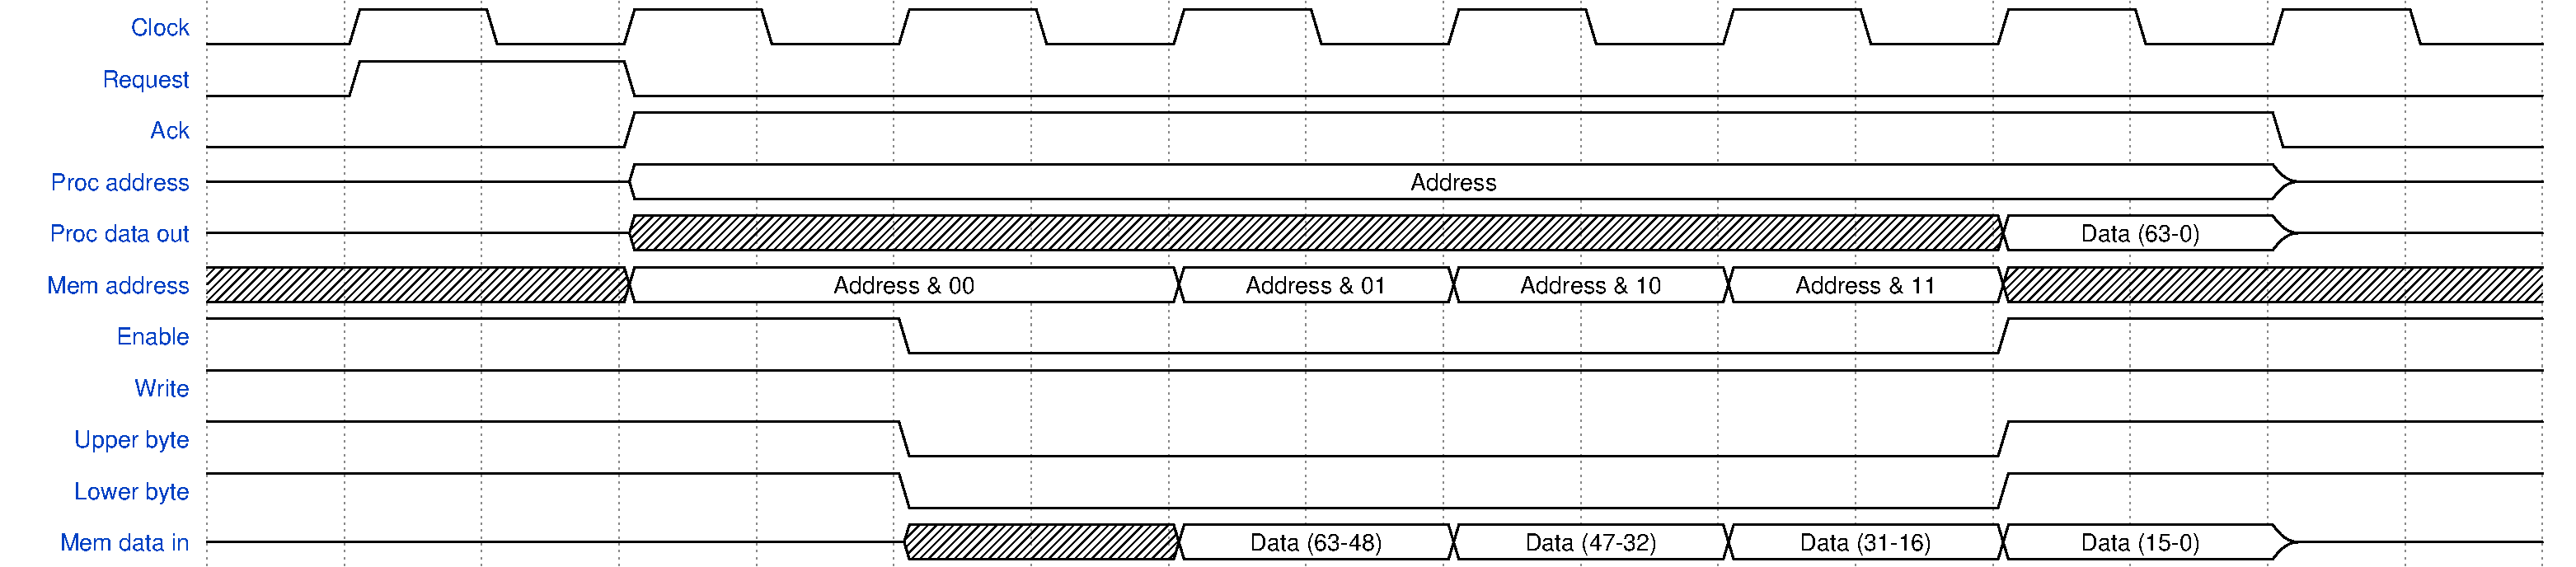
\includegraphics[width=\textwidth]{fpga/fig/timing/data_mem_read.pdf}
  \caption{Data memory read cycle}
  \label{fpga:fig:timing:dmem:read}
\end{figure}

\begin{figure}[H]
  \centering
  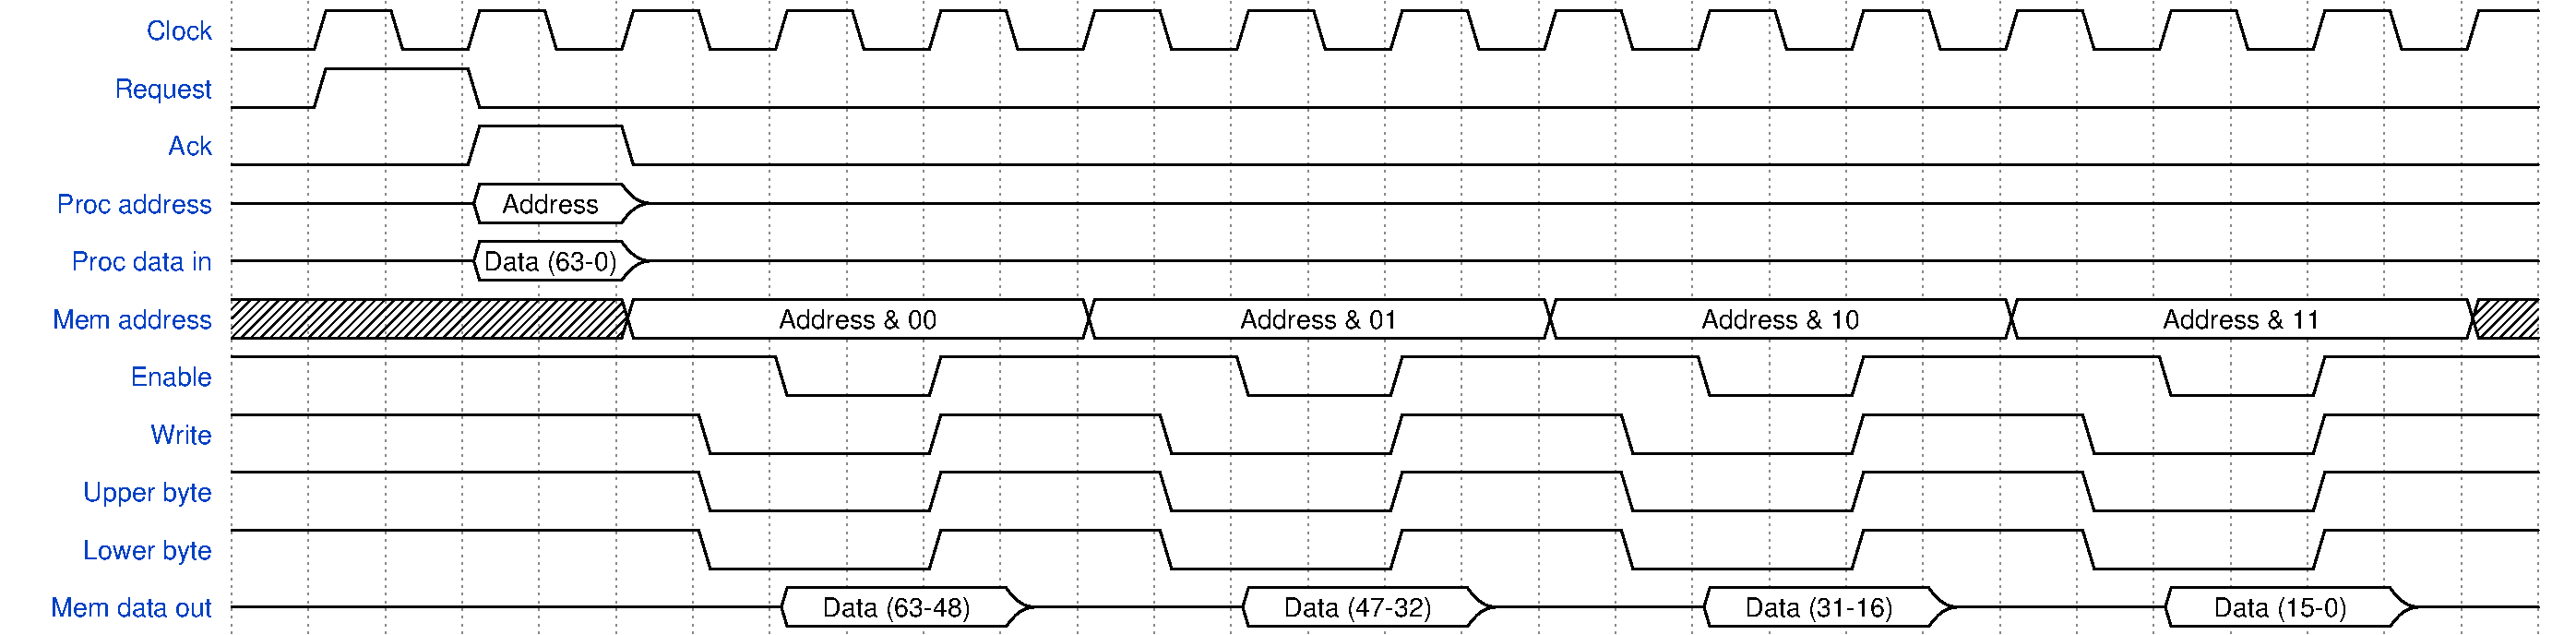
\includegraphics[width=\textwidth]{fpga/fig/timing/data_mem_write.pdf}
  \caption{Data memory write cycle}
  \label{fpga:fig:timing:dmem:write}
\end{figure}

As is immediately apparent in figures \vref{fpga:fig:timing:dmem:read} and \vref{fpga:fig:timing:dmem:write}, the number of cycles required for load and store operations are are 5 and 13 cycles, respectively.
A state machine is implemented in the \emph{data memory controller} to handle interfacing with the external memory chips.
This state machine is responsible for controlling that the different signals are set according to the diagrams.
For more detailed view of the \emph{Data memory controller}, the reader is advised to study the state machine diagram in figure \ref{fpga:fig:mem:data_memory_ctrl_state_machine} and the accompanying data path in figure \ref{fpga:fig:mem:data_memory_ctrl}.

\begin{figure}[H]
  \centering
  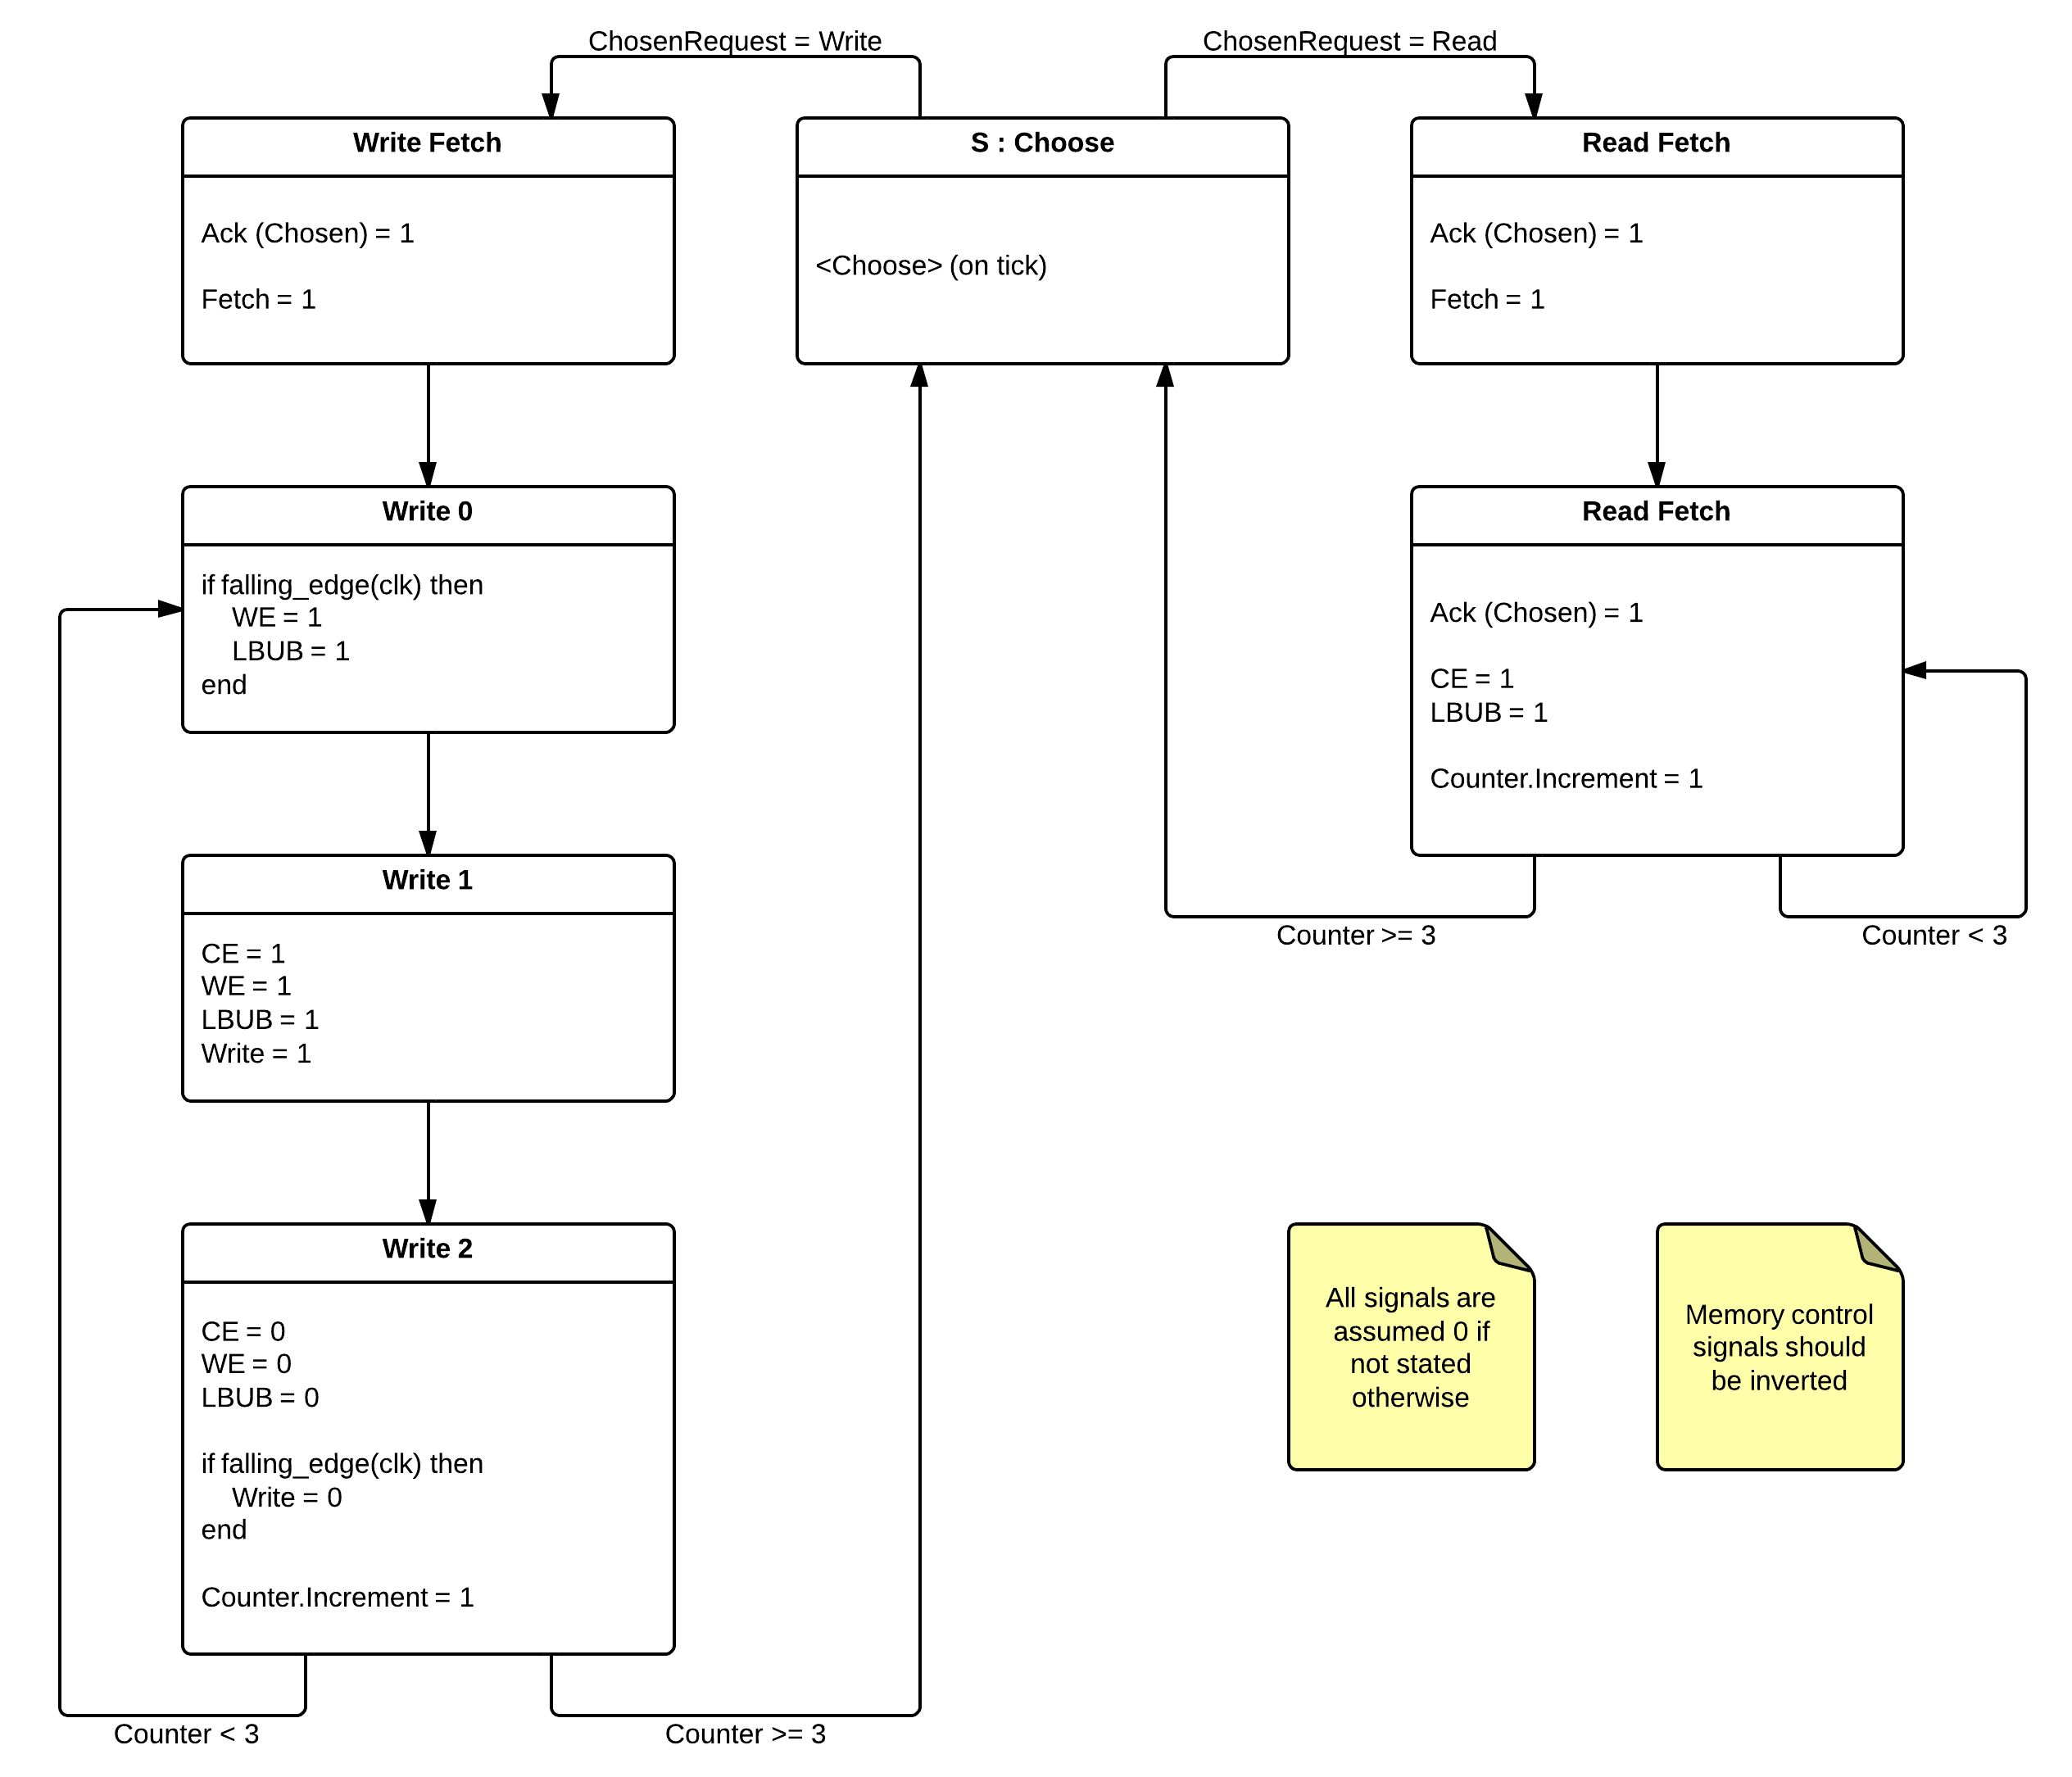
\includegraphics[width=\textwidth]{fpga/fig/memory_ctrl_state_machine.png}
  \caption{Data memory controller state machine}
  \label{fpga:fig:mem:data_memory_ctrl_state_machine}
\end{figure}


\begin{figure}[H]
  \centering
  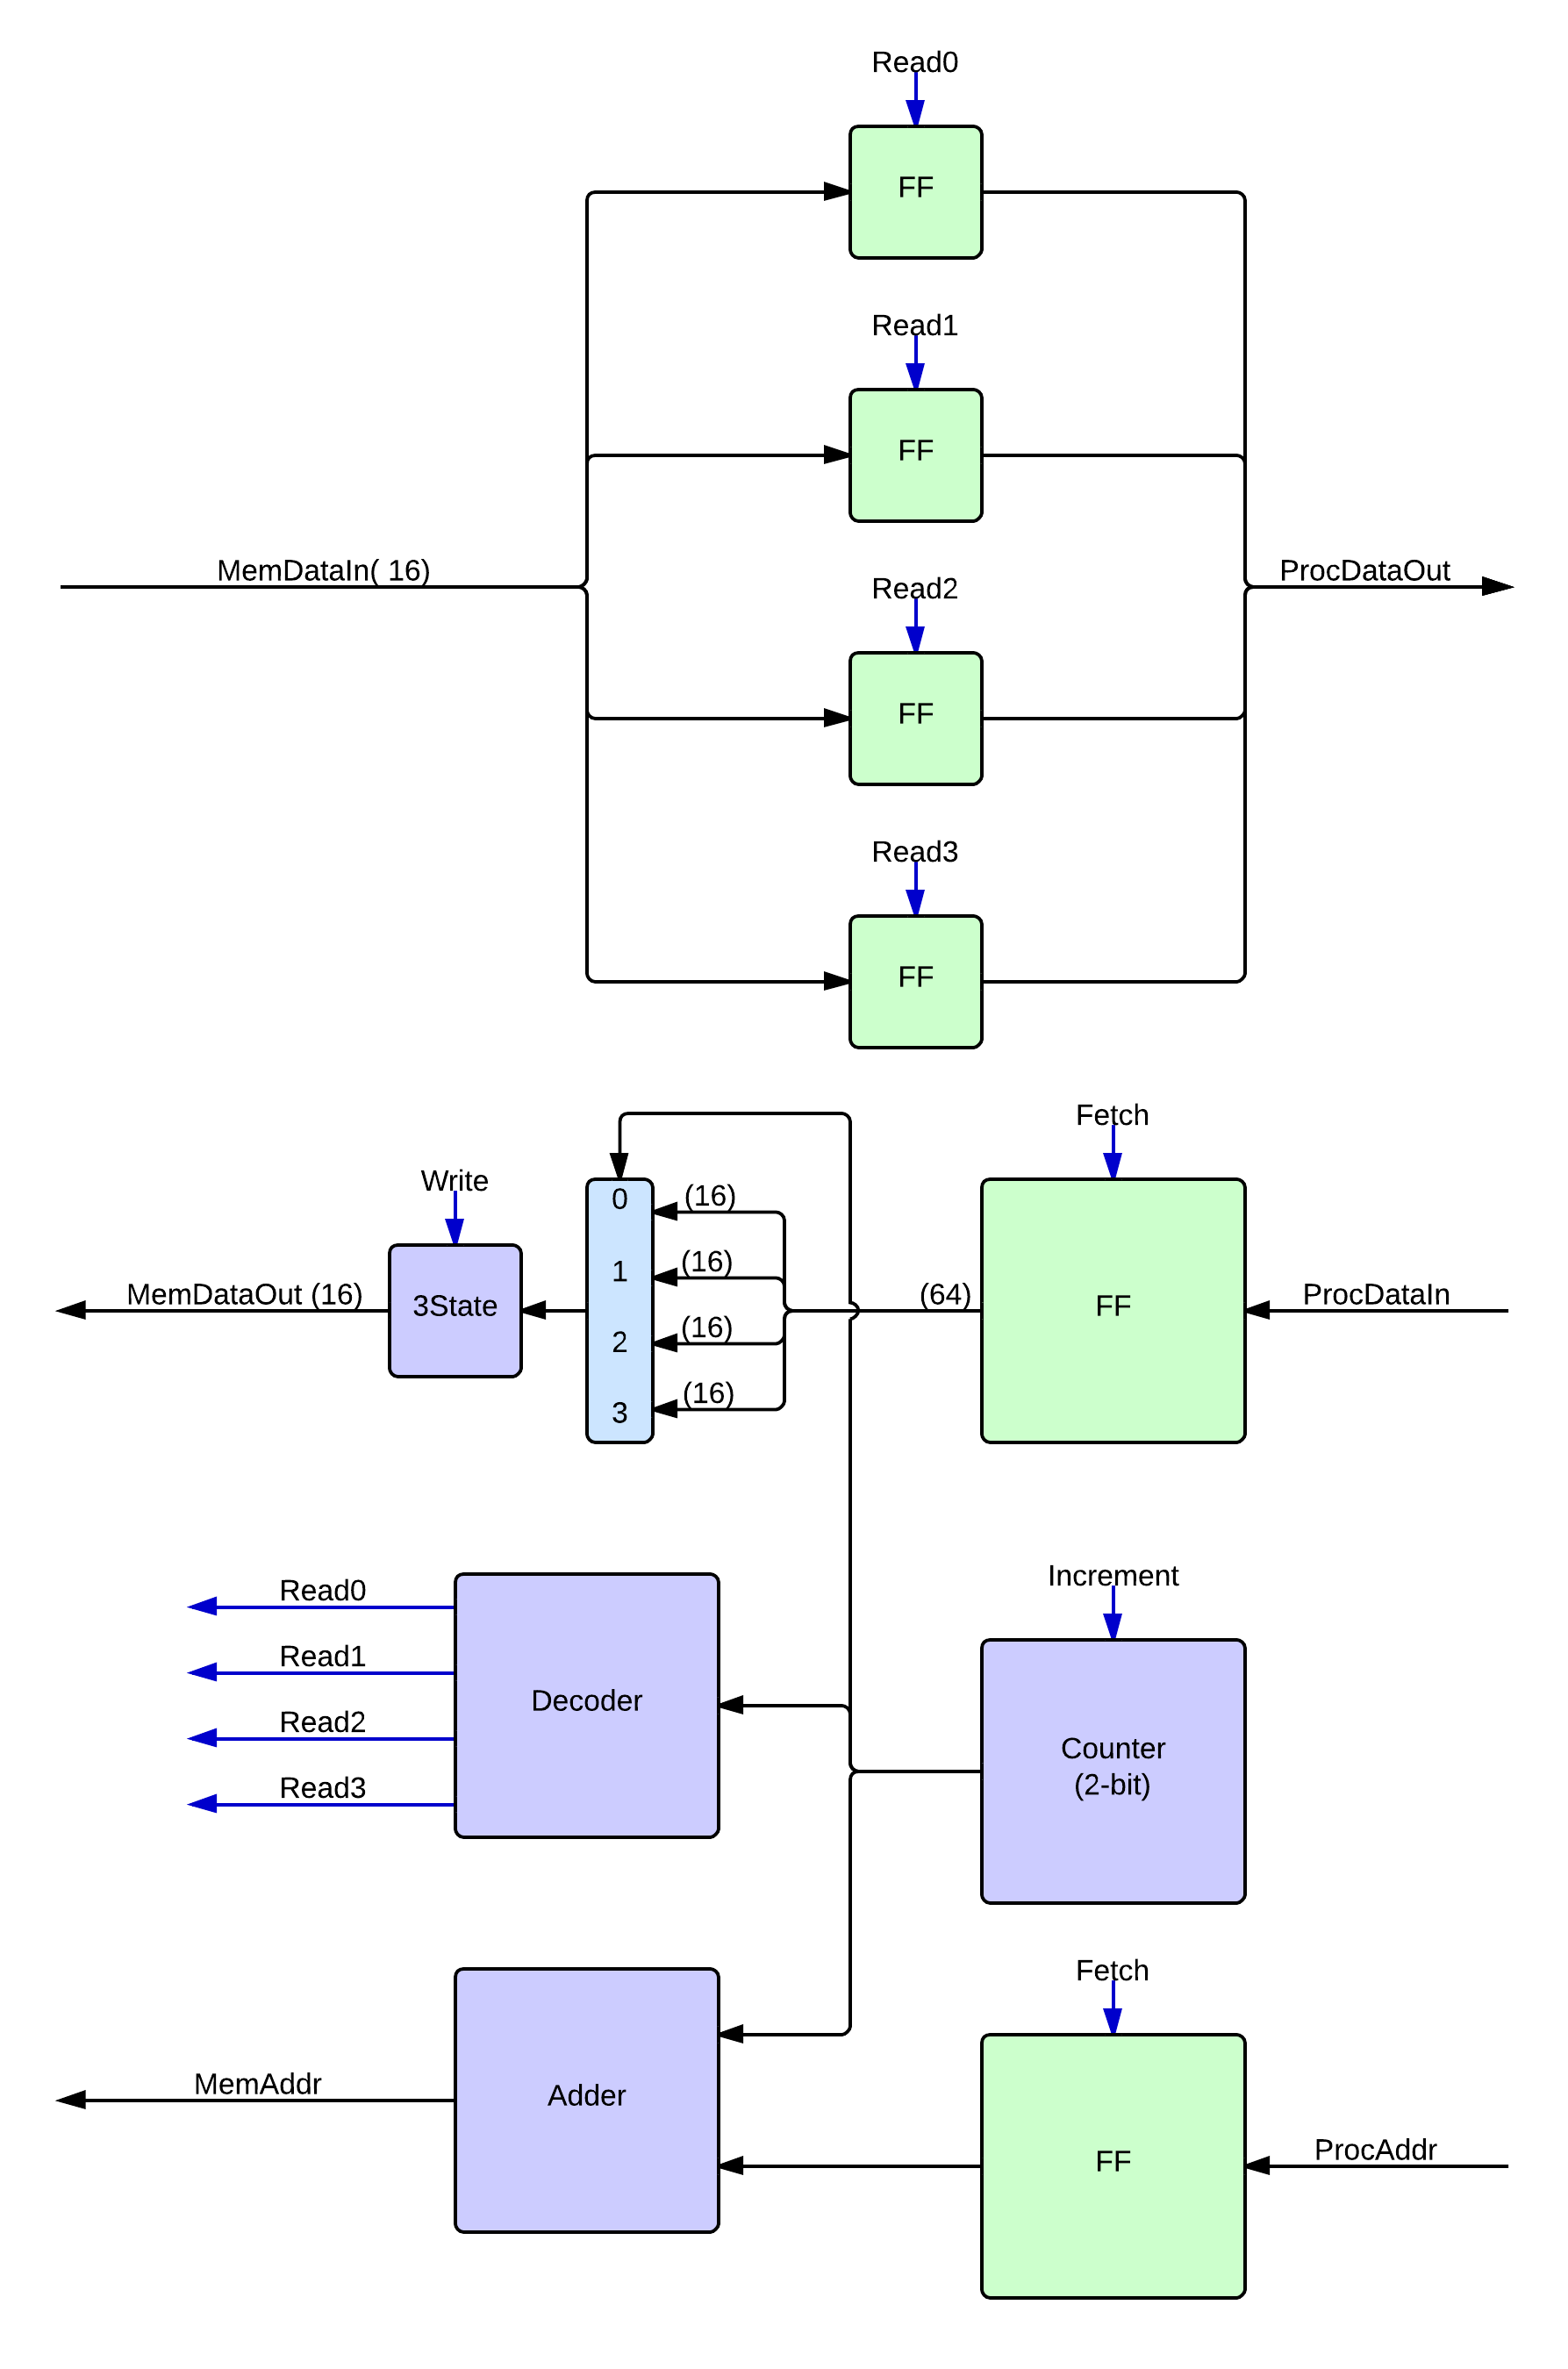
\includegraphics[width=\textwidth]{fpga/fig/memory_ctrl.png}
  \caption{Data memory controller signals mapping}
  \label{fpga:fig:mem:data_memory_ctrl}
\end{figure}


\todo{write about and ref to above graphs}


\subsection{Rated and Unrated Pools}
Individuals making up the populations are stored on the FPGA for for faster access. These are stored in \emph{BRAM} on the FPGA. This implies a lot faster access times, compared to access times to the external memory, as mentioned in (?). This is done to achieve better memory throughput when executing the algorithms. The pools are further divided into two separate \emph{BRAM} blocks, one for rated individuals, and one for un-rated. This is done to achieve even better memory throughput. The increased throughput are achieved because the different computational can work on the rated and un-rated pool simultaneously. For instance while one fitness core is storing a ranked individual, while another fitness core is fetching a new individual for ranking. 

\todo{More details and better explanation} 

Both the rated pool and the unrated pool is associated with the a controller, referred as the \emph{Genetic controller}. As with the data controller, this controller is responsible for granting access for the rated and unrated pool. This buses in question are, however, not the same as those used to access the data memory. The genetic controller use their own separate buses. The controller is based on mostly the same idea as the data controller described in section (?). The when performing genetic operations, the fitness cores need to request the data bus by using two request signals. The combination of these signals refer to the operation the fitness core requests from the genetic controller. 

The genetic cores continuously performs a round-robin in order to grant bus to the requesting fitness core. The logic surrounding the different operations are implemented as an state machine to divide the operations in different clock cycles. This is the same method as used in the data controller.







The state machine can be seen in figure(?)




\subsection{PRNG Module}
The genetic algorithms need diversity in the search space in order to be able to converge to a solution. To achieve this, the architecture need some way of creating sufficiently random numbers. These generated numbers do not need to be true randoms number, this implies that a psudo number generator will suffice. 

    
 

\subsection{Fitness Core} \label{fpga:fitness:ss:design_of_the_fitness_core}
    \subsection{Design of fitness core}

The design of the fitness core is highly influenced by MIPS.
The core is designed as a five stage pipeline.
The goal is to make it as simple as possible, and at the same time harvest efficiency by instruction level parallelism.
The more advanced features like branch prediction and instruction scheduling are not taken into consideration while designing the CPU.
The hazard detection schemes will be made simple.
The hazard resolutions will be made in software as well as in hardware.
The plan is to simply stall when we encounter any hazards in the pipeline.
The assembler will handle the most obvious ones to achieve efficiency, while the hardware will simply stall when hazards are detected.

\fxnote {The hazard scheme may change if time}
 \label{fpga:subsection:fitness_core}


\subsection{The Genetic Pipeline}
\label{fpga:subsection:genetic_pipeline}
\todo{some words about the genetics accelerator}
The galapagos architecture includes a highly specialised pipeline for performing genetic operations. The pipeline is based on the observation that selection, crossover, and mutation works similar for a specific subset of problems. These can therefore be implemented as hardware accelerators constructed for performing one specific task. Constructing such accelerators has been proven to be very beneficial regarding performance. Designing specialised hardware is usually simpler and thereby more effective than constructing general purpose components.\todo{Bullshit ?} This pipeline will effectively relieve the general cores, the fitness cores, from computing the evolution of individuals. The idea is that these will make the fitness cores able to only focus on the computation of fitness ranking, which is considered computational intensive. In the mean time the \emph{genetic pipeline} can produce new data for ranking. These operations could have been performed by the processor, however, the processor is badly suited for these kind of operations. Note that the instructions in the pipeline actually uses 5 cycles in order to complete propagate through the pipeline. It is a far better to only use one cycle in order to complete the one specific operation.  

The genetic pipeline is constructed with three specialised cores for performing selection, crossover, and mutation. These are operations that occurs frequently in genetic algorithms. These are connected to two internal memory banks on the \emph{FPGA}, namely the unrated and rated pool.


-Abstraction for the programmer. Simpler to program.
-Do not need components like ALU
- effective 
- Less control over the genetic pipeline
- 



\subsubsection {Selection Core} \label{fpga:selection:ss:selection_core}
    \input{fpga/selection-core} \label{fpga:subsection:selection_core}

\subsubsection{Crossover Core} \label{fpga:crossover:ss:crossover_core}
    \input{fpga/crossover-core} \label{fpga:subsection:crossover_core}

\subsubsection{Mutation Core}\label{fpga:mutation:ss:mutation_core}
    \input{fpga/mutation-core} \label{fpga:subsection:mutation_core}




\subsection{Parallelism}
\todo{awkwardly placed section.. move it somewhere else?}
The Barricelli is a MIMD computer, which means that it can execute multiple different instruction streams on multiple different data streams simultaneously, in parallel.
The four\cn fitness cores in the archtecture have each their own program counters and may load different data independantly of eachother.
They all share the same data and instruction memory, however, which makes the Barricelli a shared memory model MIMD computer.
Additionally, the genetic pipeline contains multiple specialized cores, which can also execute independant, less general instruction streams on independant data.

 \label{fpga:section:cpu_architecture}

%%Fitness core subsection
\subsection{Design of fitness core}

The design of the fitness core is highly influenced by MIPS.
The core is designed as a five stage pipeline.
The goal is to make it as simple as possible, and at the same time harvest efficiency by instruction level parallelism.
The more advanced features like branch prediction and instruction scheduling are not taken into consideration while designing the CPU.
The hazard detection schemes will be made simple.
The hazard resolutions will be made in software as well as in hardware.
The plan is to simply stall when we encounter any hazards in the pipeline.
The assembler will handle the most obvious ones to achieve efficiency, while the hardware will simply stall when hazards are detected.

\fxnote {The hazard scheme may change if time}
 \label{fpga:subsection:fitness_core}

%%Selection core subsection
\subsection {Design of the selection core} \label{fpga:selection:ss:selection_core}

The selection core is designed based on a tournament selection algorithm. It is designed to select an chromosome from a random position in the rated pool. The current best and the random selected is compared to each other with use of an comparator. The best chromosome is stored and used in the next tournament round. After some number of tournaments the current best is transferred to the crossover core. The selection core is actually responsible for letting the rest of the genetic pipeline know when it can fetch the next chromosome. 

The selection core is designed with efficiency in mind. The overall time spent in the genetic pipeline must be smaller than the time spent ranking the chromosomes. Note that the fitness cores are connected to the same memory bus as the genetic pipeline. This could potentially lead to a memory bottleneck resulting in starvation. The selection core tries to overcome this fact by reducing the memory access to a minimum. Note that the selection core has reserved the memory bus during the ongoing tournament. This implies that port used by the selection core is unavailable to others during this time. It is designed to not use the memory more than it absolutely have to. For instance, if the current fitness value is greater than the fitness value just fetched. The selection core will not bother fetching the accompanying chromosome. Ensuring that the memory resources are not wasted. This is accomplished with an \emph{state machine}. 



\subsubsection{Data Path}
Upon the beginning of the data path design, the group wanted to determine the the components required to perform the selection. In this specific case the group decided to design a data path able to perform a tournament selection. The resulting architecture is made as simple as possible.  It is composed of \emph{flip flops}, \emph{control unit} and an \emph{comparator}. The different components are connected as seen in figure.




\fxnote{Add figure of selection core}


\subsubsection{Control Unit} \label{fpga:selection:sss:control_unit}



\subsubsection {Comparator} \label{fpga:selection:sss:comparator}



\subsubsection{Case study} \label{fpga:selection:sss:case_study}



 \label{fpga:subsection:selection_core}

%%Crossover core subsection
The crossover Core is the next part in the genetics accelerator after the selection cores. Two inputs are forwarded from the two selections cores as "parents", and two outputs are the "children" of the inputs, containing bits from both parents. All the bits from both the parents are forwarded in the children, but in some parts the bit-patterns are switched on the children, based a selected crossover function and on a random input from the PRNG. Henceforth this is called crossover.

There are three distinct crossover functions that are implented: Split, doublesplit and function.

\paragraph{\textit{Split Fucntion}}
\begin{figure}[H]
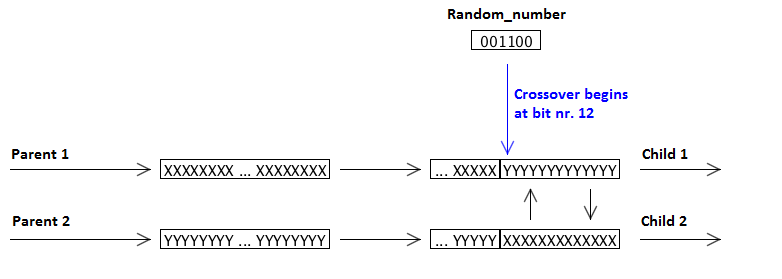
\includegraphics[width=\textwidth]{fpga/fig/crossover_split.png}
\caption{Crossover split function}
\label{fig_crossover_split}
\end{figure}

The first function, crossover split, performs crossover from a selected bit number in the children and until the edge (bit number 0). This can be seen in figure \ref{fig_crossover_split}. The values in the parents are represented with X's and Y's, and a single X or Y can have the value 0 or 1, independent of each other.
The bit number for starting crossover is based on the value of a 6-bit input random\_number, which is provided by the PRNG. This value ranges from 0 to 63.

\todo Describe how it technically works??

\paragraph{\textit{Double-split Fucntion}}
\begin{figure}[H]
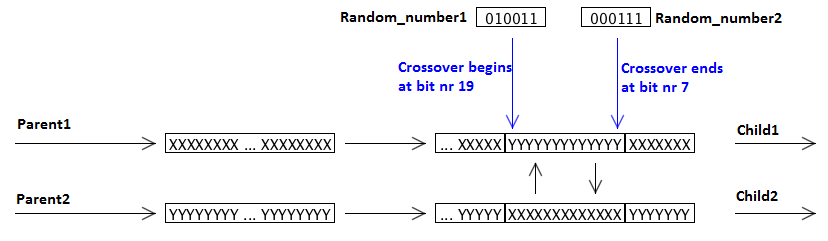
\includegraphics[width=\textwidth]{fpga/fig/crossover_doublesplit.png}
\caption{Crossover double-split function}
\label{fig_crossover_doublesplit}
\end{figure}

The second function, crossover double-split, is similar to the crossover\_split-function, but in additionally to having a starting bit for crossover, it also has an ending bit where the crossover starts, instead of reaching the edge at bit nr. 0. PRNG provides with 2 6-bit inputs, random\_number1 and random\_number2, whose values selects the starting bit and the ending bit for the crossover. These values range from 0 to 63, and if both are the same, then only one bit will be selected for crossover.

\todo Describe how it technically works??

\paragraph{\textit{XOR Fucntion}}
\begin{figure}[H]
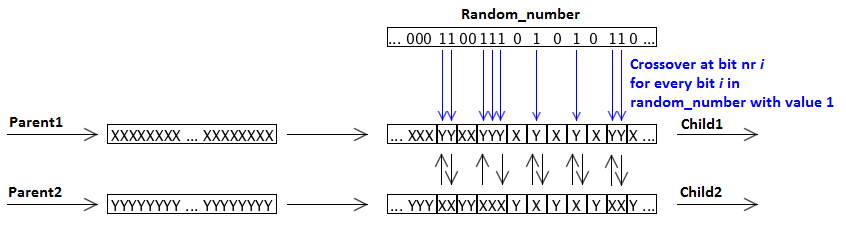
\includegraphics[width=\textwidth]{fpga/fig/crossover_xor.png}
\caption{Crossover XOR function}
\label{fig_crossover_xor}
\end{figure}

The third function, crossover XOR, performs crossover bit by bit, based on the 64-bit input random\_number. For each bit number \textit{i} in random\_number that has the value 1, the function will perform crossover on the children at the same bit number \textit{i}. This function is called XOR because of use of XOR-gates in earlier version of the function, and the principle is still the same: For each bit number \textit{i} in the child, the value will the bit number \textit{i} from one and only one parent. And which parent it is depends on the value of bit number \textit{i} in random\_number.

\todo Describe how it technically works??

\paragraph{\textit{Crossover Core Toplevel}}

The crossover core is implemented on the genetics accelerator as a toplevel containing 3 subcores, one for each function, as well as a fourth path with no crossover. In addition to the two parent inputs and 64-bit input random\_number, the toplevel has a control\_number input used for determining which crossover function is to be used: Split, doublesplit, xor, "party mode" or no crossover at all. Party mode is choosing crossover function at random, based on the 2 LS bits in the random\_number. In this way, whenever inputs are sent through the crossover\_toplevel, different functions may be used at different times. These are the control values:
\begin{itemize}
\item 000 - Split
\item 001 - Double-split
\item 010 - XOR
\item 011 - No crossover
\item 1XX - Party mode, in which case these are the random control values:
    \begin{itemize}
    \item 00 - Split
    \item 01 - Doublesplit
    \item 10 - XOR
    \item 11 - No crossover
    \end{itemize}
\end{itemize} \label{fpga:subsection:crossover_core}

%%Mutation core subsection
The mutation core is the final part in the genetics accelerator. The mutation core takes in a forwarded child from the crossover core as input and may perform mutation on a few selected bits before passing on the result. 

\begin{figure}[H]
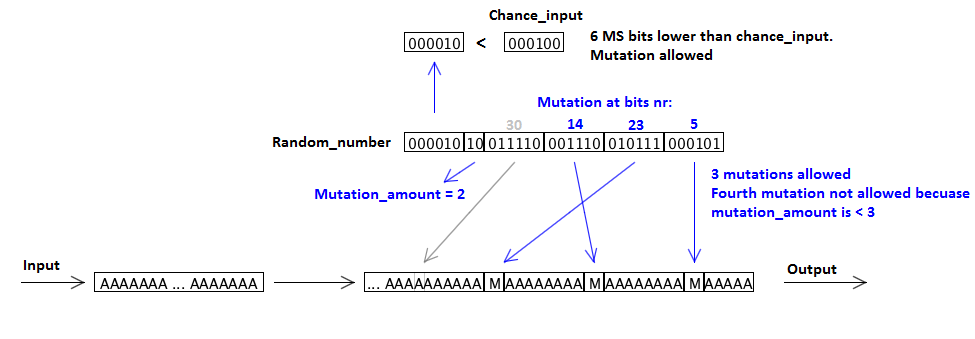
\includegraphics[width=\textwidth]{fpga/fig/mutation.png}
\caption{Mutation core function concept}
\label{Fig_Mutation}
\end{figure}

In addition to the the 64-bit child, the mutation core also takes in a 32-bit random\_number and a 6-bit chance\_input as inputs. As it can be seen in the example in figure \ref{Fig_Mutation}, all bits that are not mutated are represented by an A, and mutated bits are represented with M. The values in each A or M can be 0 or 1, independent of each other. The value M at bit number \emph{i} is the opposite of the original value A at same bit number \emph{i} in the input.
The 6 first bits in the random\_number is compared to the chance\_input, and mutation happens only if the value of these bits are less than the chance input. For each different value in chance\_input, the user may increase or decrease the chance of mutation by about 1,5\%, or $(1 / 2^6)$. If the chance input is set to 000000, no mutation will ever happen, and the user may in this way disable the mutation core.

The next two bits in the random number (bits 25-24) are used to determine how many mutations will happen. There are 4 different values, therefore there can be 1-4 mutations.
The next 24 bits are used to determine which bits are to be mutated. 6 bits are used for finding each bit number. This is similar to what is done in the split and doublesplit functions in the crossover core. These values are numbered, representing their bit field:
\begin{itemize}
\item Nr. 1: 5-0
\item Nr. 2: 11-6
\item Nr. 3: 17-12
\item Nr. 4: 23-18
\end{itemize}
These are numbered after the amount of allowed mutation. Nr. 1 will always happen when a mutation occurs, while nr. 4 happens only when the amount\_number allows for 4 mutations.

Note that if more than one of these numbers point to the same bit to be mutated, the output M will still be the inverted from the original input. For instance, if both numbers 1 and 2 (bits 11-6 and 5-0) have the value 000110, and therefore point at bit number 6, the same mutation will still happen as if only one of these numbers were 000110. If the input bit was 1, the mutated will be 0, and vice versa.
In the example provided in figure \ref{Fig_Mutation}, the 6 first bits of the random\_number are less than the chance\_input, therefore a mutation happens. Bits 23-0 have the values 30, 14, 23 and 5. Because the value of bits 25-24 is 10 (mutation\_amount has value 2), there will be 3 mutations, and the fourth does not occur (though the figure shows where it would have occured if allowed).

\begin{figure}[H]
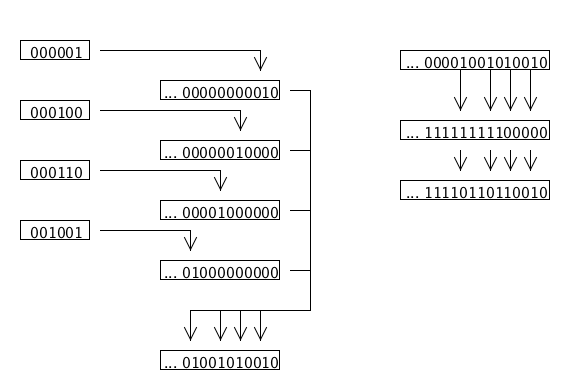
\includegraphics[width=\textwidth]{fpga/fig/mutation_mask.png}
\caption{Setting mutation}
\label{fig_mutation_mask}
\end{figure}

The mutation core is implemented by use of four shifter variables, one for each possible mutation, and set so that only one bit is 1 for the output. A final mutation is set by combining the outputs from the shifter variables by using OR-funftion, and the mutation\_amount determines how many of these outputs are combined. Figure \ref{fig_mutation_mask} shows an example where bits 1, 4, 6 and 9 are set for mutation. In this case the final output is set by combining the input and mutation with the XOR-fuction, so that for each bit \emph{i}, the bit is set to 1 if and only if bit \emph{i} is set in either the input or the mutation, but not both. This can be seen in figure \ref{fig_mutation_perform}.

\begin{figure}[H]
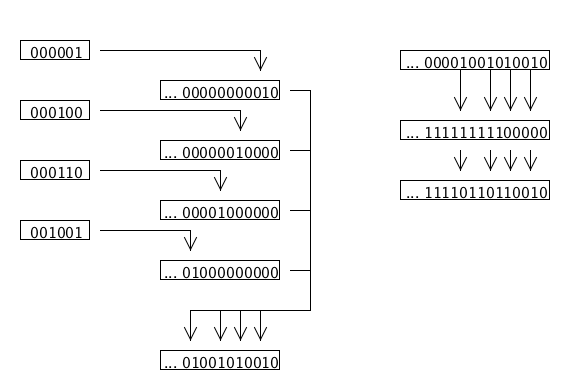
\includegraphics[width=\textwidth]{fpga/fig/mutation_mask.png}
\caption{Performing mutation}
\label{fig_mutation_perform}
\end{figure}

\todo{ "Selected bit number" needs to somehow be defined in the description of the shifter variable + ShifterVariable needs to be described.} \label{fpga:subsection:mutation_core}

#if 0
PCB
    Design Choices
        IO devices
        Internal Communication
        External communication
        Memory
    Power Supply
    Power Plane
    Footprints
        
    Process
        System design
        PCB design and routing
        Soldering
    Problems and workaround
#endif


\chapter{Input/Output}
	\section{Input and Output}
The PCB contains a microcontroller used to manage all input and output between the FPGA and the IO devices shown in Figure ~\vref{figure:system-overview}.
The microcontroller listens on all IO channels for input, and acts on the input, either forwarding the request to another device or performing memory operations on the FPGA's memory.

\subsection{Initial requirements}
The assignment required a microcontroller to handle IO for the FPGA.
To minimize the amount of things that could go wrong, much of the initial work was focused on finding a few reliable and relatively simple data connections.

Specifically, the microcontroller was required to be able to put some program and data on the FPGA's memory, and then later output values from the data memory through the proper communication lines.
The I/O devices together with the microcontroller and it's software should be able to provide a reliable and stable I/O connection between the outside world and the FPGA.

\subsection{Communication channels}
\subsubsection{SD Card}
The SD card reader is primarily used as a storage for programs that are to be uploaded on the FPGA.
However, it might also be used to store memory snapshots in order to look how the genetic algorithm converges to a solution over time.

The Energy Micro Application Note on Fat and SD cards, and its example code, describes an implementation of the FatFS library on the Giant Gecko microcontroller.\cite{an0030}

\paragraph{FatFS}\cite{fatfs-web}

FatFS is a generic FAT file system for microcontrollers, with a generic interface for the FAT operations, and a hardware specific interface for disk I/O.
Because of this structure, the system is easily portable.
To add read and write a FAT system on some disk drive, FatFS needs the following functions:

\begin{table}[H]
    \begin{tabular}{| l | l |}
        \hline
        disk\_initialize & Initialize disk drive \\
        \hline
        disk\_status & Get disk status \\
        \hline
        disk\_read & Read sectors on disk \\
        \hline
        disk\_write & Write sectors on disk \\
        \hline
        disk\_ioctl & Control device dependent features \\
        \hline
        get\_fattime & Get current time for FAT \\
        \hline
    \end{tabular}
    \caption{Overview of disk I/O functions}
\end{table}

\subsubsection{USB}
The USB is the main communication line with a host computer, allowing the host computer to start running programs on the FPGA and receive snapshots of the memory periodically.
The microcontroller has a built in USB controller~\cite{efm32gg990-datasheet} and energy micro has supplied an application note~\cite{an0065} with code for utilizing the included USB controller in order to act as a USB device.

\subsubsection{Serial}
The serial port is meant as a backup solution in case USB doesn't work, with the exact same opportunities, but with an older, simpler interface.
The microcontroller used in the project has a built in UART Receiver/Transmitter\cite{efm32gg990-datasheet} which is easily activated with code from AN0045~\cite{an0045}.

\subsubsection{LEDs and buttons}
The most primitive form of IO we have are the on-board LEDs and buttons.
They allow a quick and easy way to verify that a program is running, and possibly letting the user change execution modes or the program on the FPGA with the buttons.
All code interfacing with the LEDs and buttons are simple code either setting or reading the value of GPIO pins.
The LEDs are driven by General Purpose IO pins on the SCU, requiring a minimal amount of code in order to get a working output, which is especially handy in the early stages of implementation.

\subsubsection{FPGA}
There are 41 wires between the FPGA and the SCU in order to facilitate communication (see Table~\ref{tab:scu-fpga-link} for a complete list of all the connections).
The FPGA has no way of signalling that it wants to output something, so the SCU is responsible for periodically halting the CPU on the FPGA and reading from it's memory.

\subsubsection{J-link}
In order to program and debug the programs on the SCU, we utilize the built-in pins for debugging using J-Link\texttrademark as described in AN0043~\cite{an0043}.
It can also be used as a form of last resort emergency output as it makes it possible to display text that is printed by the program running on the SCU.

\section{FPGA Control}
The only way of communication with the FPGA is with direct memory access to the FPGA's data and instruction memory.
All the data is transferred directly over the SCU's GPIO pins, without any form for memory mapping or built-in bus interfaces.
This is mostly due to the fact that we did not do enough research early in the design process and recognized that we could use something like External Bus Interface to access the memory.

Access to the FPGA's memory is controlled by the signals seen in Table~\ref{tab:scu-fpga-link}.
It should be noted that there are two states to access the FPGA's instruction memory, the upper and lower half.
This is because the instruction memory stores 32 bits per address while the SRAM chips only stores 16 bits per address (see Section~\ref{subsec:fpga-instruction-memory} for more details on the instruction memory).

The SRAM data sheet~\cite{sram-datasheet} specifies that the data signal has to be stable for at least 10ns in order to complete a write.
This means that it is not necessary to worry about timing when accessing the SRAM since changing the signal more than every 10ns requires a clock speed of 100MHz since we can at most change the output of a single pin every cycle.

\begin{table}[H]
    \begin{tabular}{| l | l | l |}
        \hline
        Signal & Bus width & \\
        \hline
        FPGA enable & 1 & Enables the FPGA on high, disables it on low\\
        \hline
        FPGA State & 2 & \pbox{20cm}{00: Processor enable\\01: Instruction memory upper half access\\10: Instruction memory lower half access\\11: Data memory access}\\
        \hline
        Chip enable & 1 & The chip enable signal in to the selected memory block.\\
        \hline
        Write enable & 1 & The write enable signal in to the selected memory block.\\
        \hline
        Address & 19 & The address bus to the selected memory block.\\
        \hline
        Data & 16 & The data bus to the selected memory block.\\
        \hline
        LBUB & 1 & The LB and the UB signal to the selected memory block.\\
        \hline
    \end{tabular}
    \label{tab:scu-fpga-link}
    \caption{Lines between the SCU and FPGA}
\end{table}

\section{IO Program}
\begin{figure}[H]
    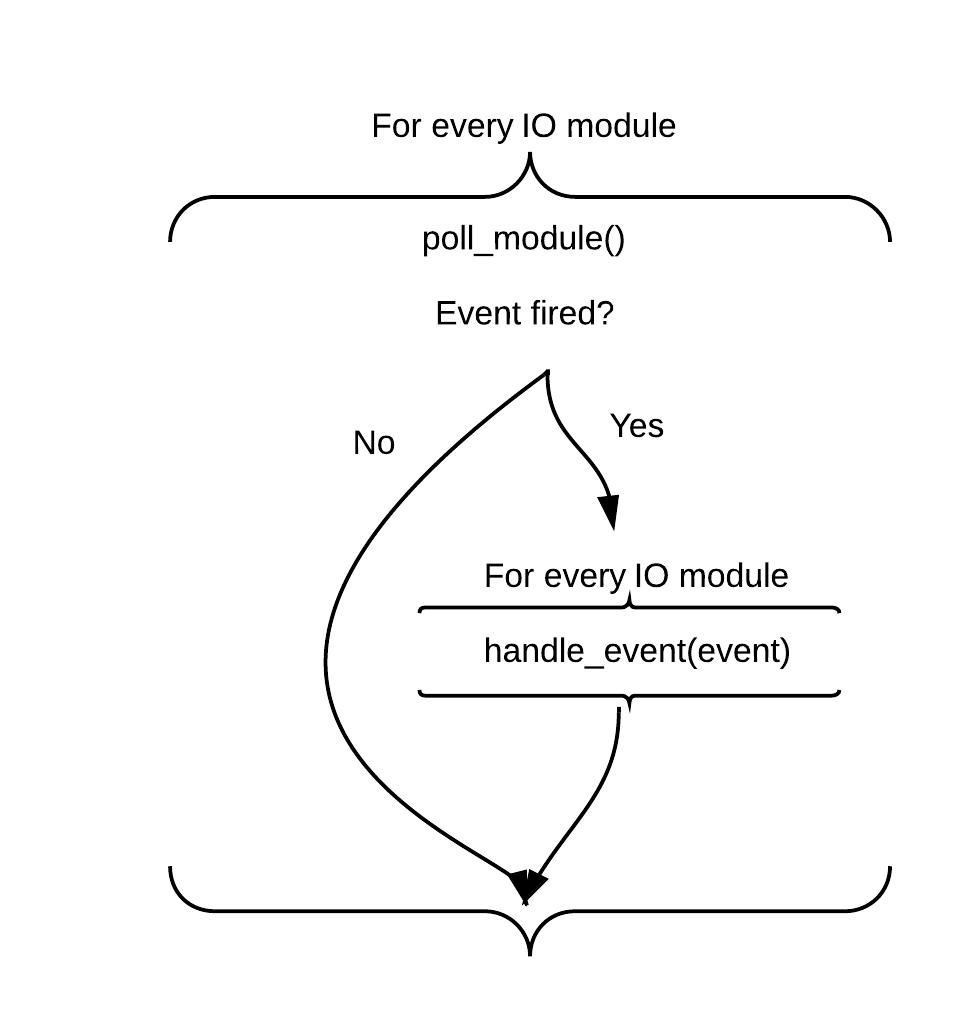
\includegraphics[width=\textwidth]{io/fig/program.png}
    \caption{The body of the IO program's main loop}
\end{figure}

The IO program was designed to be as simple as possible in order to decrease the amount of things that could go wrong.
The main idea is that every IO device is required to define two functions in order to be used: a function to poll for input and a function that is called whenever a device reports input.

In order to enable sending messages between different IO units, the poll functions return a pointer which may point to any object in memory, which allows other modules to read the data given that they know what type of data the pointer points to.

\section{Design decision}
\subsection{Selection of microcontroller}
The microcontroller chosen was chosen as it was the microcontroller we had available to test with on the development kit.
It was also the microcontroller with most available GPIO pins for the package we had to use, which would give us the most possibilities for communication.

\subsection{Operating system}
Early in the process, a discussion arose about how it could be beneficial to run an operating system on the microcontroller such that familiar programs could be run directly on it.
A scenario pitched was to have network access, and then be able to talk to the machine remotely using programs such as \textit{SSH} or \textit{telnet}.
However, the Linux distribution available for the Energy Micro microcontroller was found lacking in the features we wanted, and the microcontroller lacks network support.
It was therefore decided that running an OS was unnecessary as there were few rewards and little to gain from it.

\subsection{FPGA Communication}
During the initial design phase, the link between the FPGA and SCU was designed to be as simple as possible.
The final version was the the 41 wires mapping all the signals needed for directly accessing the SRAM chips.
\todo{Make up some reasons here, should probably defend not using EBI}

\section{Issues}
\subsection{Crystal}
In the design phase it was decided to go with just a single high frequency crystal oscillator.
Unfortunately the crystal that was selected had a clock frequency in the kHz range, instead of the MHz range, which was what was intended.
Luckily the microcontroller has a built-in RC oscillator, so the crystal oscillator was not essential to get code running on the microcontroller.

\subsection{USB Circuitry not working}
While mapping the PCB circuitry, only the pins available for GPIO were included initially, but this did not include the vbus and vregi pins.
The pins were connected to capacitors, and a quick hack soldering the appropriate lines to the USB header was tried without success.

\subsection{No UART}
The microcontroller believes that data is being outputted and calls the data sent callback function.
There also seems to be a signal going out to the RS-232 interface, but there is no data being received on the other end.

\todo{no SD card}

\subsection{Memory access}
\todo{Diagnostics, possibly not just here/not here at all.}
Tried:
\begin{itemize}
    \item Adding delays
    \item Reading immediately after write to verify write,
    \item Mapping control signals to LED on FPGA to verify that they work
    \item Flashing the instruction memory on the FPGA so we just have to read data memory, not write
\end{itemize}


\chapter{Additional Components}
    \section{\Gls{galapagos assembler}}

The \Gls{galapagos assembler} is an assembler for \Gls{galapagos} Assembly that was written for this project.
It asembles galapagos assembly to be run on the programmable fitness cores of the Barricelli computer.
The assembler is written in Python. 
It is designed with a modular, object-oriented software architecture, which makes it easily extensible and modifiable.
Indeed, during the short time it has been published on the Internet, it has already been forked and adapted for use for other instruction set architectures and assembly languages.\cn \todo{yes, I'm talking about how I cooked galapagos-as for use in dmkons -- sigve}
The assembler supports the entire \Gls{galapagos} instruction set.

With a an assembler available, opportunities for performance optimizations through instruction re-ordering are made available.
The idea is that instructions within a simple code block, i.e. a branch-less block of consecutive instructions with no labels, instructions may be carefully re-ordered to minimize data hazards.
The assembler does not perform these instruction re-orderings.
This is because the forwarding unit in the processor architecture already resolves many of the same issues that the assembler would work around using instruction re-ordering.

The only non-control related hazards that the forwarding unit doesn't already resolve are use-after-load conflicts.
A use-after-load conflict is a conflict where the processor plans the execute a data load from memory, and then use the result from that load in the immediately proceding execution.
When this happens, the result from the memory load is not yet ready when the execution is planned to execute.
This hazard is resolved off-line by the assembler.
It can detect use-after-load hazards during assembly, and will insert a \gls{nop} between the load and use instructions, forcing the processor to wait until the data is available.

\Gls{galapagos assembler} is available in PyPi, the leading python package index.
This means that it is easily installable for end users using \texttt{pip}, the python package manager.
Installation is as simple as running \texttt{pip install galapagos-assembler} in a terminal where pip is available.

The source code of the \Gls{galapagos assembler} can be found in appendix \vref{appendix:galapagos-assembler-source-code}.

\section{Case}

\todo{this}


\part{Results and Discussion}

\chapter{Tests}
	When designing a computer with a custom architecture from scratch, it is important to continually test and evaluate the correctness of the solution at all possible stages, to ensure that final product is a success.
This section documents and explaines the rationale behind the different types of tests that have been performed.

\section{Testing the Processor}

Baricelli's processor has been tested at four different levels: \gls{VHDL}-based unit test simulations of the different subcomponents,  \gls{VHDL}-based integration test simulations of each processing unit, \gls{VHDL}-based system test simulations of the entire system interfacing against a mock SCU and mock memory, and finally physical integration tests of the processor programmed onto the FPGA of the Barricelli.

\todo{what about timing simulations?}

\subsection{\gls{VHDL}-based Subcomponent Unit Test Simulations}

Unit testing VHDL entites is extremely important in a large and complex design like the Barricelli.
For this project, almost every component, perhaps except the most trivial entities, is tested in an automated or semi-automated VHDL test bench.
A tool was developed to ease the automation of VHDL test running and validation, modeled after the leading test runners in the software industry, such as JUnit\cn and Karma\cn.
This tool enabled tests to be written using easy-to-use self-evaluating tests that compare signals at specific times against expected values.

The goal of these unit tests is to ensure that the building block components work as expected when reacting to specified input.

Screenshots of simulations of these tests can be found in Appendix \ref{appendix:test-bench-documentation}.
\todo{ Make sure screenshots of as many tests as possible are available. If not, then we probably have to do references from the following tables}
\todo{we need to stash results somewhere}.

\subsubsection{Fitness Core Components}
\todo{ Insert text and tables for components used in Fitness Core}

\subsubsection{Genetic Pipepline Components}
\todo{ Insert text and tables for components used in Genetics Pipeline}
\paragraph{Selection Core}
\paragraph{Genetic Pipeline Controller?}
\paragraph{Unrated pool?}
\paragraph{Rated pool?}

\todo{ Hmm...seems I overdid the length in the tables. Again!....(T-Bear)}
\begin{table}[H]
  \begin{tabular}{r | p{9cm}}
    \noalign{\smallskip}\hline\noalign{\smallskip}
    
    What to test:  & Check if crossover split function performs crossover correctly, 
                        from correct bit \\

    \noalign{\smallskip}\hline\noalign{\smallskip}

    How to test:   &    Changes in any input should cause change in the outputs.
                        Therefore parent inputs and random\_number will be changed
                        during test. 
                        \\
                      
    \noalign{\smallskip}\hline\noalign{\smallskip}

    Pass criteria: &    The output for child1 should have output from parent1 and child2
                        from parent2 before crossover point, and child1 should have
                        output from parent2 and child2 from parent1 after crossover
                        point. 
                        The starting point, which is the first bit in the crossover,
                        should always be the bit number equal to the value of
                        random\_number.
                        \\
    \noalign{\smallskip}\hline\noalign{\smallskip}
    
    Results: &      Successful. 
                    Changes in parents cause expected changes in children, and starting 
                    point for crossover is always equal to the value of random\_number
                    \\
   \noalign{\smallskip}\hline\noalign{\smallskip}
  
  
  
  \end{tabular}
  \caption{Crossover Core Split function}
  \label{testing:components:genetic_pipeline:crossover_core_split}
\end{table}

\begin{table}[H]
  \begin{tabular}{r | p{9cm}}
    \noalign{\smallskip}\hline\noalign{\smallskip}
    
    What to test:  & Check if Crossover Double-Split Function performs crossover
                     correctly, from correct starting bit to correct ending bit \\

    \noalign{\smallskip}\hline\noalign{\smallskip}

    How to test:   &    Changes in any input should cause change in the outputs.
                        Therefore parent inputs and random\_numbers will be changed
                        during test.  
                        \\
                      
    \noalign{\smallskip}\hline\noalign{\smallskip}

    Pass criteria: &    The output for child1 should have output from parent1 and child2
                        from parent2 before crossover starting point and after ending 
                        point, and child1 should have output from parent2 and child2
                        from parent1 between the crossover starting point and ending
                        point. 
                        The random\_number with the highest value should always be the 
                        starting point, and the one with the lowest value should always
                        be the ending point. 
                        These points, which are the first and the last bit in the 
                        crossover, should always be the bit numbers equal to the value     
                        of the random\_numbers. 
                        If both have same value, then only one bit location will have a
                        crossover
                        \\
    \noalign{\smallskip}\hline\noalign{\smallskip}
    
    Results: &      Successful. 
                    Changes in parents cause expected changes in children, and starting 
                    point for crossover is always equal to the value of the highest 
                    random\_number, and ending point for crossover is always equal to 
                    the value of the lowest random\_number
                    \\
   \noalign{\smallskip}\hline\noalign{\smallskip}
  
  
  
  \end{tabular}
  \caption{Crossover Core Double-Split function}
  \label{testing:components:genetic_pipeline:crossover_core_doublesplit}
\end{table}

\begin{table}[H]
  \begin{tabular}{r | p{9cm}}
    \noalign{\smallskip}\hline\noalign{\smallskip}
    
    What to test:  & Check if Crossover XOR Function performs crossover
                     correctly, from correct starting bit to correct ending bit \\

    \noalign{\smallskip}\hline\noalign{\smallskip}

    How to test:   &    Changes in any input should cause change in the outputs.
                        Therefore parent inputs and random\_number will be changed
                        during test.  
                        \\
                      
    \noalign{\smallskip}\hline\noalign{\smallskip}

    Pass criteria: &    The output for child1 should have output from parent1 and child2
                        from parent2 for each bit \emph{i}, where in the random\_number 
                        the value is 0, and child1 should have output from parent2 and 
                        child2 from parent1 for each bit \emph{i}, where in the 
                        random\_number the value is 1.
                        \\
    \noalign{\smallskip}\hline\noalign{\smallskip}
    
    Results: &      Successfull.
                    Changes in parents cause expected changes in children, and for each
                    bit \emph{i} in the random\_number, there are crossover at same bit    
                    \emph{i} from the parents to the children.
                    \\
   \noalign{\smallskip}\hline\noalign{\smallskip}
  
  
  
  \end{tabular}
  \caption{Crossover Core XOR function}
  \label{testing:components:genetic_pipeline:crossover_core_xor}
\end{table}

\begin{table}[H]
  \begin{tabular}{r | p{8cm}}
    \noalign{\smallskip}\hline\noalign{\smallskip}
    
    What to test:  & Check if Crossover Toplevel selects correct crossover function
                     based on control\_input, and random\_number when in "Party Mode"\\

    \noalign{\smallskip}\hline\noalign{\smallskip}

    How to test:   &    Changes in parents are not relevant, since this test is not 
                        inteded to test the functions themselves, only the function 
                        selection.
                        Every input of control\_input will be tested.
                        Changes in random\_number will be done with focus on the 2 LS 
                        bits when control\_input is "1XX", and in party mode.
                        \\
                      
    \noalign{\smallskip}\hline\noalign{\smallskip}

    Pass criteria: &    When control\_input is set to 000, or 1XX and random\_input-bits 
                        to 00, crossover should be split with the value of the 6 LS bits 
                        from random\_number used for starting point.
                        When control\_input is set to 001, or 1XX and random\_input-bits 
                        to 01, crossover should be double-split, with the value of the 
                        12 LS bits from random\_number used for starting and ending 
                        point.
                        When control\_input is set to 010, or 1XX and random\_input-bits 
                        to 10, crossover should be xor, with crossover on every bit 
                        numbers that are 1 in random\_number.
                        When control\_input is set to 011, or 1XX and random\_input-bits 
                        to 11 there should be no crossover at all, and output children 
                        should be equal to each their input parent.
                        \\
    \noalign{\smallskip}\hline\noalign{\smallskip}
    
    Results: &      Successfull. 
                    Each value in control\_input was tested, and set the expected 
                    function. When set to 1XX, every value on the 2 LS bits in the 
                    random\_number was tested, and set the expected function.
                    \\
   \noalign{\smallskip}\hline\noalign{\smallskip}
  
  
  
  \end{tabular}
  \caption{Crossover Core Toplevel}
  \label{testing:components:genetic_pipeline:crossover_core_toplevel}
\end{table}

\begin{table}[H]
  \begin{tabular}{r | p{9cm}}
    \noalign{\smallskip}\hline\noalign{\smallskip}
    
    What to test:  & Check if Mutation Core selects mutates when allowed, mutates the 
                     correct amount of bits, and the correct bit numbers, all based
                     on chance\_input and random\_number.\\

    \noalign{\smallskip}\hline\noalign{\smallskip}

    How to test:   &    Changes on input will change output. Therefore input will have 
                        changes.
                        Changes in random\_number and chance\_input  will be done with
                        focus to test allowing or denying mutation.
                        Changes in random\_number will also be done to test amount of 
                        allowed mutations, and to test selecting the locations of the 
                        mutations
                        \\
                      
    \noalign{\smallskip}\hline\noalign{\smallskip}

    Pass criteria: &    When the P first bits in random\_number is equal to or higher 
                        than chance\_input (size P), there should be no mutation at all.
                        When mutation is allowed, the next two bits should allow these 
                        amount of mutations: 1-4 depending on values 00-11.
                        Bits 23-0 select four bit locations for mutations, and the 
                        output should have opposite value on these locations compared to
                        the input.
                        If more than one bit location pointer has the same value, the 
                        same bit location should still have the mutation on the output.
                                                \\
    \noalign{\smallskip}\hline\noalign{\smallskip}
    
    Results: &      Successful. 
                    Mutation is allowed only when the P first bits are lower than the
                    chance\_input, the correct amount of mutations were set and each 
                    four bit locations were selected correctly as expected by bits 23-0
                    \\
   \noalign{\smallskip}\hline\noalign{\smallskip}
  
  
  \end{tabular}
  \caption{Mutation Core}
  \label{testing:components:genetic_pipeline:mutation_core}
\end{table}



\subsubsection{Components stolen from AREA 51}
\todo{ Insert text and tables for components used elsewhere}

\subsection{\gls{VHDL}-based Processing Unit Integration Test Simulations}

Each processing unit, which each consists of several interconnected subcomponents, has been simulated for integration testing.
The goal of these tests are to verify that the different subcomponents interface correctly with eachother, and that the behaviour of the supercomponent is as expected.

\subsubsection{Testing the Fitness Core}

\todo{about tb\_fitness\_core.vhd}

\subsubsection{Testing the Genetics Pipeline}

\todo{about tb\_genetics\_pipeline.vhd}

\subsection{\gls{VHDL}-based System test Simulations}
\label{section:testing:fpga:system-tests}

The toplevel simulation test bench of the barricelli computer, which simulates the entire FPGA as a black box interfacing against the external components, supports pre-loading entire programs into a mocked instruction memory component.
The \Gls{galapagos assembler} supports outputting assembled programs compiled to one of these mock memory components, meaning that testing new programs in a simulated environment is an easy and fun process.

\todo{the title of the test should be above the table in which its results are displayed, not just as the caption (rendered below) of the table}

A formal description of the system tests performed at this level can be found in tables
\ref{testing:fitness:pipeline_test},
\ref{testing:fitness:branch_taken},
\ref{testing:fitness:branch_not_taken},
\ref{testing:fitness:conditional_taken},
\ref{testing:fitness:conditional_not_taken},
\ref{testing:fitness:load_data},
\ref{testing:fitness:store_data},
\ref{testing:fitness:store_gene},
and
\ref{testing:fitness:load_gene}.

\begin{table}[H]
  \begin{tabular}{r | p{8cm}}
    \noalign{\smallskip}\hline\noalign{\smallskip}
    
    What to test:  & Observe that RRI and RRR instructions propagate correctly through the pipeline, 
                     and produce the correct result.\\

    \noalign{\smallskip}\hline\noalign{\smallskip}

    How to test:  & The program in listing \todo{create listing}, consisting of both RRR and RRI instructions,
                    are loaded into memory with the test framework. The execution of the instructions are observed with
                    isim.\\

    \noalign{\smallskip}\hline\noalign{\smallskip}

    Pass criteria: & The flow of data is according to the architecture presented in figure. \todo{add reference}
                   Register 1, 2, 3 are loaded with 9, 10 and 19, respectively.   \\
    
     \noalign{\smallskip}\hline\noalign{\smallskip}

    Results: &  What are the result of the test. \\
   \noalign{\smallskip}\hline\noalign{\smallskip}
  
  
  \end{tabular}
  \caption{RRR and RRI instructions}
  \label{testing:fitness:pipeline_test}
\end{table}


\begin{table}[H]
  \begin{tabular}{r | p{8cm}}
    \noalign{\smallskip}\hline\noalign{\smallskip}
    
    What to test:  & Check if the branch address is calculated correctly, and an conditional
                     jump is performed to this address. \\

    \noalign{\smallskip}\hline\noalign{\smallskip}

    How to test:   &  The program in listing \todo{create listing}, is loaded into a test bench.
                      This simple program consists of a simple loop performing some arithmetic
                      operations that store values to registers. The execution of the
                      program is simulated with isim to verify the result \\

    \noalign{\smallskip}\hline\noalign{\smallskip}

    Pass criteria: &  The branch is taken. The instructions located in the $fetch stage$, 
                       $decode stage$, and $execute stage$ are flushed. The results in registers
                       should be X, X, and X in registers X, X and X, respectively. \\

    \noalign{\smallskip}\hline\noalign{\smallskip}
    
    Results: &  Registers X, X, and X is contained in the registers. The instructions in $fetch
                stage$, $decode stage$ and $execute stage$ does not perform any  
                changes to the register file. \\
   \noalign{\smallskip}\hline\noalign{\smallskip}
  
  
  
  \end{tabular}
  \caption{Branch taken}
  \label{testing:fitness:branch_taken}
\end{table}

\begin{table}[H]
  \begin{tabular}{r | p{8cm}}
    \noalign{\smallskip}\hline\noalign{\smallskip}
    
    What to test:  & Check if the conditional jump is disregarded when performing conditional
                     that always evaluate to false.\\

    \noalign{\smallskip}\hline\noalign{\smallskip}

    How to test:   &  The program in listing \todo{create listing}, is loaded into a test bench. 
                       The simple program consists of conditionals that evaluate to false. The
                       execution of the program is simulated with isim, and the results are
                       verified. \\

    \noalign{\smallskip}\hline\noalign{\smallskip}

    Pass criteria: & Execution of the program should not store any data to the registers.\\

    \noalign{\smallskip}\hline\noalign{\smallskip}
    
    Results: &   No data is stored to registers. \\
   \noalign{\smallskip}\hline\noalign{\smallskip}
  
  
  
  \end{tabular}
  \caption{Branch not taken}
  \label{testing:fitness:branch_not_taken}
\end{table}

\begin{table}[H]
  \begin{tabular}{r | p{8cm}}
    \noalign{\smallskip}\hline\noalign{\smallskip}
    
    What to test:  & Check if conditional instruction are executed when they
                     always are evaluated to true.   \\

    \noalign{\smallskip}\hline\noalign{\smallskip}

    How to test:  & The program in listing \todo{create listing}, is loaded into test bench. The 
                    simple program consists of a set with simple conditional instructions that
                    always evaluate to true. The execution of the program is simulated with isim, 
                    and the result is verified. 
    \\

    \noalign{\smallskip}\hline\noalign{\smallskip}

    Pass criteria: & The instructions propagates normally through the pipeline. The different instruction are executed and their results are written to the register file. \\

    \noalign{\smallskip}\hline\noalign{\smallskip}
    
    Results: &  \\
   \noalign{\smallskip}\hline\noalign{\smallskip}
  
  
  
  \end{tabular}
  \caption{Conditional instruction executed }
  \label{testing:fitness:conditional_taken}
\end{table}

\begin{table}[H]
  \begin{tabular}{r | p{8cm}}
    \noalign{\smallskip}\hline\noalign{\smallskip}
    
    What to test:  & Check if conditional instructions are executed when they always evaluate to 
                     false. \\

    \noalign{\smallskip}\hline\noalign{\smallskip}

    How to test:   &  The program in listing \ref{testing:listing:conditional-not_executed}, is loaded into a test bench. 
                       The simple program consists of a set of simple conditional instructions that         
                       always evaluate to false. The execution of the program is observed in 
                       ISim,and the results are verified. The content of register r1 is observed.\\

    \noalign{\smallskip}\hline\noalign{\smallskip}

    Pass criteria: & The second instruction, the conditional \emph{ADDI}, is not executed. The content of register r1 is 1.  \\

    \noalign{\smallskip}\hline\noalign{\smallskip}
    
    Results: & The content of register r1 is 1. The conditional \emph{ADDI} instruction is not executed. .  \\
   \noalign{\smallskip}\hline\noalign{\smallskip}
  
  
  
  \end{tabular}
  \caption{Conditional instruction not executed}
  \label{testing:fitness:conditional_not_taken}
\end{table}

\begin{table}[H]
  \begin{tabular}{r | p{8cm}}
    \noalign{\smallskip}\hline\noalign{\smallskip}
    
    What to test:  & Observe that LOAD instructions is able to read from memory, and load the
                     memory content into the specified registers.  \\

    \noalign{\smallskip}\hline\noalign{\smallskip}

    How to test:   & The program in listing \todo{create listing}, consisting mainly of LOAD
                     instructions. These are loaded into a testbench, and simulated with 
                     isim. \\
                     

    \noalign{\smallskip}\hline\noalign{\smallskip}

    Pass criteria: &  \\

    \noalign{\smallskip}\hline\noalign{\smallskip}
    
    Results: &  \\
   \noalign{\smallskip}\hline\noalign{\smallskip}
  
  
  
  \end{tabular}
  \caption{Load data}
  \label{testing:fitness:load_data}
\end{table}

\begin{table}[H]
  \begin{tabular}{r | p{8cm}}
    \noalign{\smallskip}\hline\noalign{\smallskip}
    
    What to test:  & \\

    \noalign{\smallskip}\hline\noalign{\smallskip}

    How to test:   & \\

    \noalign{\smallskip}\hline\noalign{\smallskip}

    Pass criteria: & \\

    \noalign{\smallskip}\hline\noalign{\smallskip}
    
    Results: &  \\
   \noalign{\smallskip}\hline\noalign{\smallskip}
  
  
  
  \end{tabular}
  \caption{Store data}
  \label{testing:fitness:pipeline_test}
\end{table}
\begin{table}[H]
  \begin{tabular}{r | p{8cm}}
    \noalign{\smallskip}\hline\noalign{\smallskip}
    
    What to test:  &  \\

    \noalign{\smallskip}\hline\noalign{\smallskip}

    How to test:   &  \\

    \noalign{\smallskip}\hline\noalign{\smallskip}

    Pass criteria: &  \\

    \noalign{\smallskip}\hline\noalign{\smallskip}
    
    Results: &  \\
   \noalign{\smallskip}\hline\noalign{\smallskip}
  
  
  
  \end{tabular}
  \caption{Store gene}
  \label{testing:fitness:store_gene}
\end{table}

\begin{table}[H]
  \begin{tabular}{r | p{8cm}}
    \noalign{\smallskip}\hline\noalign{\smallskip}
    
    What to test:  &  Observe that a gene is fetched from the unrated code, and stored in the
                      specified register\\

    \noalign{\smallskip}\hline\noalign{\smallskip}

    How to test:   &  The program in listing \ref{testing:listing:load-gene}, consisting of LOAD GENE
                      instructions. These are loaded into a test bench and simulated with 
                      ISim. The content of the location of the distributed counters are checked against the data 
                      loaded to the fitness cores.  \\

    \noalign{\smallskip}\hline\noalign{\smallskip}

    Pass criteria: &  The data fetched from the rated pool is the same gene transmitted to the
                      fitness core. \\

    \noalign{\smallskip}\hline\noalign{\smallskip}
    
    Results: &  Success \\
   \noalign{\smallskip}\hline\noalign{\smallskip}
  
  
  
  \end{tabular}
  \caption{Load gene}
  \label{testing:fitness:load_gene}
\end{table}

\begin{table}[H]
\center
\begin{tabular}{|l | c | c | c | c |c|}
    \hline
    Clock cycle & IF & ID & EX & MEM & WB \\
    \hline
    3 & ADD 3, 1, 2  & ADDI 2, 10 & ADDI 1, 10   &              &              \\
    4 &              & ADD 3, 1, 2  & ADDI 2, 10    & ADDI 1, 10   &              \\
    5 &              &              & ADD 3, 1, 2   & ADDI 2, 10   & ADDI 1, 10    \\
    6 &              &              &               & ADD 3, 1, 2  & ADDI 2, 10    \\
    7 &              &              &               &              & ADD 3, 1, 2  \\
    \hline
\end{tabular}
\caption{Instruction flow}
\label{testing:tbl:instrflow}
\end{table}




\begin{table}[H]
  \begin{tabular}{r | p{8cm}}
    \noalign{\smallskip}\hline\noalign{\smallskip}
    
    What to test:  &  Test a specific genetic problem using the Galapagos architecture. 
                      The problem in question aims to find a specific color, $magic pink$, by 
                      genetic evolution. \\

    \noalign{\smallskip}\hline\noalign{\smallskip}

    How to test:   &  The program in listing \ref{testing:listing:color-search} is loaded into a test bench. The
    programs consists of both genetic and fitness related instructions. Program is executed and
    verified with ISim. The registers containing the best chromosome and fitness values are studied
    during the run. \\

    \noalign{\smallskip}\hline\noalign{\smallskip}

    Pass criteria: &  Execution shall show an improvement of the fitness scores and the chromosomes
    as the program simulates. E.g that it converges against a solution. \\

    \noalign{\smallskip}\hline\noalign{\smallskip}
    
    Results: &   The problem converges and the color is found.\\
   \noalign{\smallskip}\hline\noalign{\smallskip}
  
  
  
  \end{tabular}
  \caption{Find color: A genetic solution}
  \label{testing:genetic:genetic_color}
\end{table}


\begin{table}[H]
  \begin{tabular}{r | p{8cm}}
    \noalign{\smallskip}\hline\noalign{\smallskip}
    
    What to test:  & Test a spesfic genetic problem using the barricelli computer. 
                     The problem in question aims to find a solution to the knapsack problem. 
                     The problems involves finding the best combination of items to put into a
                     knapsack with a weight constraint. The test start with a set of items with
                     a given score and weight. 
                      \\

    \noalign{\smallskip}\hline\noalign{\smallskip}

    How to test:  & The program in listing \todo{Add listing} is loaded into a test bench. 
                    The program consists of both genetic and fitness related instructions.
                    The program is executed and verified in isim. The registers containing the
                    best solutions are studied during the run. \\

    \noalign{\smallskip}\hline\noalign{\smallskip}

    Pass criteria: &  It is observed that the best solution converges against a better solution
                       regularly. E.g that it continuously improve for the better.  \\
    
     \noalign{\smallskip}\hline\noalign{\smallskip}

    Results: &   It is observable that it improve after a number of microseconds. It is, however, 
                 difficult to determine if this solution is good since the simulation 
                 is limited to just a few microseconds. Note that the simulations
                 create a lot of simulation related data for a small amount of simulation time.  \\
   \noalign{\smallskip}\hline\noalign{\smallskip}
  
  
  \end{tabular}
  \caption{The knapsack problem : A genetic solution}
  \label{testing:fitness:pipeline_test}
\end{table}



\subsection{Physical Integration Tests}

Finally, on the physical board, the processor was tested by running the same programs as in the system tests described in section \vref{section:testing:fpga:system-tests}.
These programs were programmed into the instruction memory of the processor by the SCU.

\section{Testing the PCB}
During and after the components were soldered on the PCB board, the board were tested to ensure that the powergrid were working as it was supposed to.
For the first test, it was checked that all the various leds on the board was working in order to verify that the board actually was powered right, and that there was
no short circuts on the power grid itself.

Some of the earliest test were also to check that the FPGA actually was working properly, and it was done by making a simple FPGA echo program to test the various pins on the fpga.
The pins on the fpga were tested by connecting a led to the various FPGA-headers. If the fpga worked correctly, the led will activate, indicating the the pins actually are operating right.
When this test was conducted on the first board that were soldered, it came out that the FPGA was not "baked on" right, and that we had to start solder a new board. 

\subsection{testing the SD card}
After the completion of the solderingprocess for the PCB a test were also conducted in order to ensure that the 
SD card were connected right, and outputting the right signals. 
--picture of fpga headers
\todo{the thing where we made a simple fpga echo program for the pins, and tested the lines from the fpga to the headers using an led. for results: we discovered a bad bake this way}

\section{Testing IO}
\subsection{IO device tests}
\test
{Buttons \& LEDs}{
    \item{Upload a program reading the state of all buttons and turning off the LEDs corresponding to the buttons pressed down while leaving the rest of the LEDs on}
    \item{Try pressing the different buttons}
}{All LEDs light up initially and turn off when the corresponding button is pressed.}
{All LEDs light up initially and turn off when the corresponding button is pressed.}

\test
{Debug connection test}{
    \item{Connect the debug pins to the appropriate pins on the energy micro development kit}
    \item{Turn the debug to OUT}
    \item{Connect to the development kit using energyAware commander}
}{EFM32GG990F1024 listed as microcontroller}
{EFM32GG990F1024 listed as microcontroller}

\test
{SD Card test}{
    \item{Edit the code from AN0030~\cite{an0030} to use correct pins}
    \item{Compile the code, upload and run it, with SD Card connected}
    \item{Confirm data on SD Card}
}{File with string ``EFM32 ...the world's most energy friendly microcontrollers !'' is added to the SD Card.}
{The SD card was not found, and the text not present on the SD Card}

\test
{USB test}{
    \item{Compile the code from AN0065~\cite{an0065}}
    \item{Upload and run it}
    \item{Run the supplied host PC program while connected to the PCB through USB}
}{The host programs runs successfully}
{The host program fails to connect through USB}

\test
{Serial test}{
    \item{Compile the code from AN0045~\cite{an0045}}
    \item{Upload and run it}
    \item{Connect the host PC to the PCB and run terminal emulator of choice}
}{"Energy Micro RS-232 - Please press a key" appears in the terminal}
{No output in terminal}

\subsection{FPGA bus}
\test
{SRAM test}{
    \item{Write a value to a range of addresses}
    \item{Read the same address and compare with the value written}
}{The values are identical}
{Most of the values are identical, with some addresses reporting the wrong value}

\test
{Running a program}{
    \item{Upload a program to fill the memory with fibonacci numbers}
    \item{Let the CPU run for a while to ensure that somehting has been written to memory.}
    \item{Read memory and check whether the fibonacci numbers are stored, the first on adress 0, the next on the next address and so on.}
}{A sequence of fibonacci numbers in the memory.}
{Seemingly random data read from the memory}


\section{Testing Additional Components}

\subsection{Galapagos Assembler}

\todo{galapagos-as has a test-suite, write about it}

\section{Additional Tests}

\subsection{The Pseudo-Random Number Generator}

A key component in any genetic algorithm worth its salt is a decent source of (pseudo-)random numbers.
The Barricelli computer has a hardware pseudo-random number generator module built into its genetics accelerator.
When designing a pseudo-random number generator, there is always a trade-off between generating ``good'' random numbers, and generating them fast.
Having high performance as a design goal\cn, it was desirable to design a pseudo-random number generator that is as fast as possible while still meeting the minimum requirements for randomness that is needed for successfully using it in a genetics algorithm application.

The pseudo-random number generator designed for the Barricelli has been tested extensively with a pseudo-random number generator test suite called DieHarder\cn.
DieHarder is a test suite which measures the ``goodness'' of a pseudo-random number generator based a number of criteria.
\todo{ what are these criteria?}

The algorithm was implemented in python and tested agains the DieHarder integration suite\cn.

The shift-based algorithm used in the pseudo-random number generator scores quite poorly in the DieHarder tests when every single bit of the output is used.
However, by only using every 7th number\cn, the algorithm ranks quite well.

Finally, some genetics algorithms convergence tests were run, also simulated in python, using the different pseudo-random algorithm candidates as a random number source in the experiments.
Based on the results from these experiments, it is safe to conclude that, while Barricelli's pseudo-random number generator algorithm may not be best-in-class for producing convincing randomness, it is definitely good enough for problem solving using genetic algorithms, and most certainly quicker than other more ``proper'' algorithms.

\todo{ dig up some numbers, show some graphs}



\todo{The contiunous ga test}


\chapter{Results}
	This section section describes the results of different measurements, calculations and tests that were run on the Barricelli computer.
It also documents the different demonstration programs that showcase and illustrate Barricelli's purpose through practical use, as well as research done in the design of Barricelli.

\section{Research}

\subsection{Steady State Genetic Algorithm}
A big question in the design of the architecture, was how to implement the genetic algorithm.
As \vref{fr7} states, the instruction set should include instructions to speed up genetic operations.
To fulfill this requirment, the algorithm would have to be directly integrated with the computer.

In the research, some papers were found that discussed Steady State Genetic Algorithms.\cite{vlsi-ga}
As these were described as being advantageous on a MIMD architecture, there was interest in further research.
However, few citations were found on how steady state algorithms performancewise related to traditional genetic algorithms.
This section documents an original research on Steady State, where both a generational and a steady state solver was implemented in Python, and used to solve a problem.

\subsubsection{Problem}
\lstinputlisting[language=Python, caption={Genetic problem}, label={lst:problem}]{continuous-ga-test/problems.py} 

The problem, implemented in listing \ref{lst:problem}, is to maximize a bit string, that is to make let have every bit be 1.
Implemented are functions for selection, crossover, mutation, creation and calculating fitness.
I. e. what is needed for a genetic search.

\subsubsection{Solvers}
\lstinputlisting[language=Python, caption={Generational solver}, label={lst:gensolver}, firstline=3, lastline=59]{continuous-ga-test/solvers.py} 

\lstinputlisting[language=Python, caption={Steady state solver}, label={lst:steadsolver}, firstline=62, lastline=108]{continuous-ga-test/solvers.py} 

In listing \ref{lst:gensolver}, there is implemented a generational version of a genetic algorithm, while in listing \ref{lst:steadsolver} there is a steady state version.
The main difference of these two solvers is how the new individuals are added to the population.
In the generational, the new individuals are inserted for the worst individuals in the old population, maintaining the population size by keeping the best of the old population if there is not enough new individuals.
The steady state version just replaces a random selected individual of the current population with the new one.

\subsubsection{Result}
\begin{table}[H]
\begin{center}
\begin{tabular}{ | c | c | }
    \hline
    Generational    & Steady State \\
    \hline
    210             & 10899 \\
    243             & 27714 \\
    238             & 2336  \\
    134             & 4210  \\
    223             & 2048  \\
    143             & 4365  \\
    285             & 1526  \\
    244             & 8733  \\
    141             & 21515 \\
    180             & 3119  \\
    \hline
\end{tabular}
\end{center}
\caption{Results of ten runs of the genetic programs}
\label{tbl:genresults}
\end{table}
After 10 runs, the generational implementation had average number of generations equal 204.1, while the steady state has a comparative result of 86.5.
The result of the steady state seems much higher than the generational, as it doesn't count generation in the same way.
To get comparable results, the work of the steady state algorithm should be divided by the population size, in this case 100.

As can be seen from table \ref{tbl:genresults}, the number of generations varies a lot more in the steady state, but as the average was significantly lower than generational, the conclusion was that steady state was better, and chosen for the project.


\section{Measurements}

This section presents the measurements found during the project.
These results are discussed in Chapter \vref{chapter:discussion}.

\subsection{Performance}

\begin{figure}[H]
    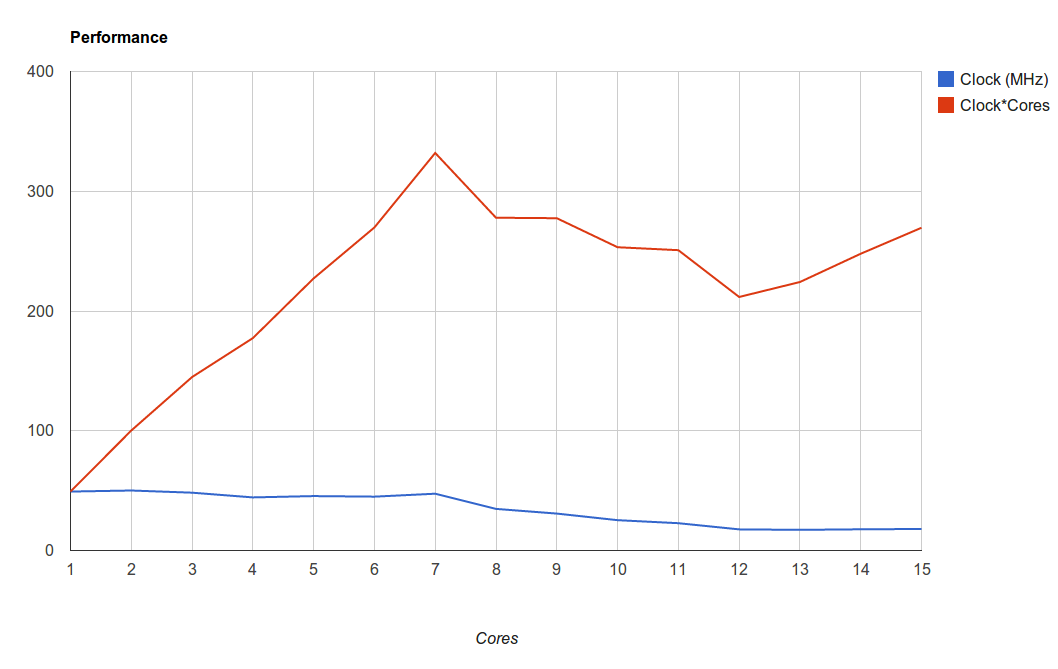
\includegraphics[width=\textwidth]{fpga/fig/performance.png}
    \caption{Total performance of Barricelli's fitness cores, as a function of number of cores}
    \label{figure:total-performance}
\end{figure}

The total performance of Barricelli's fitness cores, measured as maximum theoretical clock speed times number of clock cores, is illustrated in Figure \vref{figure:total-performance}.
This 

\todo{measure performance with different core amounts}

\todo{measure performance with and without genetics pipeline}

\todo{measure performance of same problems on consumer grade laptop}

\todo{measure performance of general program}



\section{Demonstration Programs}

This section documents the demonstration programs written for the Barricelli computer to demonstrate its functionality.
The programs are typically written in \gls{galapagos} assembly for programs running on the custom processor, and C for programs running on the \Gls{SCU}.
The source code for these demonstration programs can be found in appendix \vref{appendix:demonstration-programs-source-code}.

\subsection{Genetic Algorithm: Color Search}

The color search program is a very simple program demonstrating a basic usage of the genetics accelerator.
The program tries to find a specific color in the search-space of all 24-bit colors.

\subsubsection{Individual representation}

An individual represents a specific 24-bit color in RGB format.
The individual is coded to a 64-bit data word like in figure \vref{figure:color-search-bytefield}.

\begin{figure}[H]
    \begin{center}
        \begin{bytefield}[bitwidth=0.5em,endianness=big]{64}
            \bitheader[bitformatting={\tiny\rotatebox[origin=B]{90}}]{0, 7, 8, 15, 16, 23, 24, 63} \\
        \bitbox{40}{\color{lightgray}\rule{\width}{\height}}
            \bitbox{8}{blue}
            \bitbox{8}{green}
            \bitbox{8}{red}
        \end{bytefield}
        \caption{The binary coding of an individual for the color search problem}
        \label{figure:color-search-bytefield}
    \end{center}
\end{figure}

\subsubsection{Fitness Function}

The fitness for an individual is calculated using equation \vref{equation:color-search-fitness-function}.
The fitness a any given individual falls in the range $ [0, 768] $.

\begin{eqnarray}
\nonumber
fitness & = & 768 \\
\nonumber
        & - & |red_{individual} - red_{target}| \\
\nonumber
        & - & |green_{individual} - green_{target}| \\
        & - & |blue_{individual} - blue_{target}|
\label{equation:color-search-fitness-function}
\end{eqnarray}

\subsubsection{Results}

Figure \vref{figure:color-search} shows the evolution of the approximation suggested as an answer by the genetic algorithm.
In this problem instance the target color was magic pink, i.e. the color with color code $ rgb(255, 0, 255) $.
The program run illustrated in figure \vref{figure:color-search} ran on 7 seven cores, and the measurements are from regularly polling a single core for its current best solution.
Figure \vref{figure:color-search} clearly illustrates a typical trait of genetic algorithm approximations: they are quite good at finding decent approximations, but iterating to improve accuracy of the result is a game of diminishing returns.
The algorithm quickly finds a decent approximation of the target color, but finding the exact value down to the last bit still takes time.

\begin{figure}[H]
    \begin{center}
        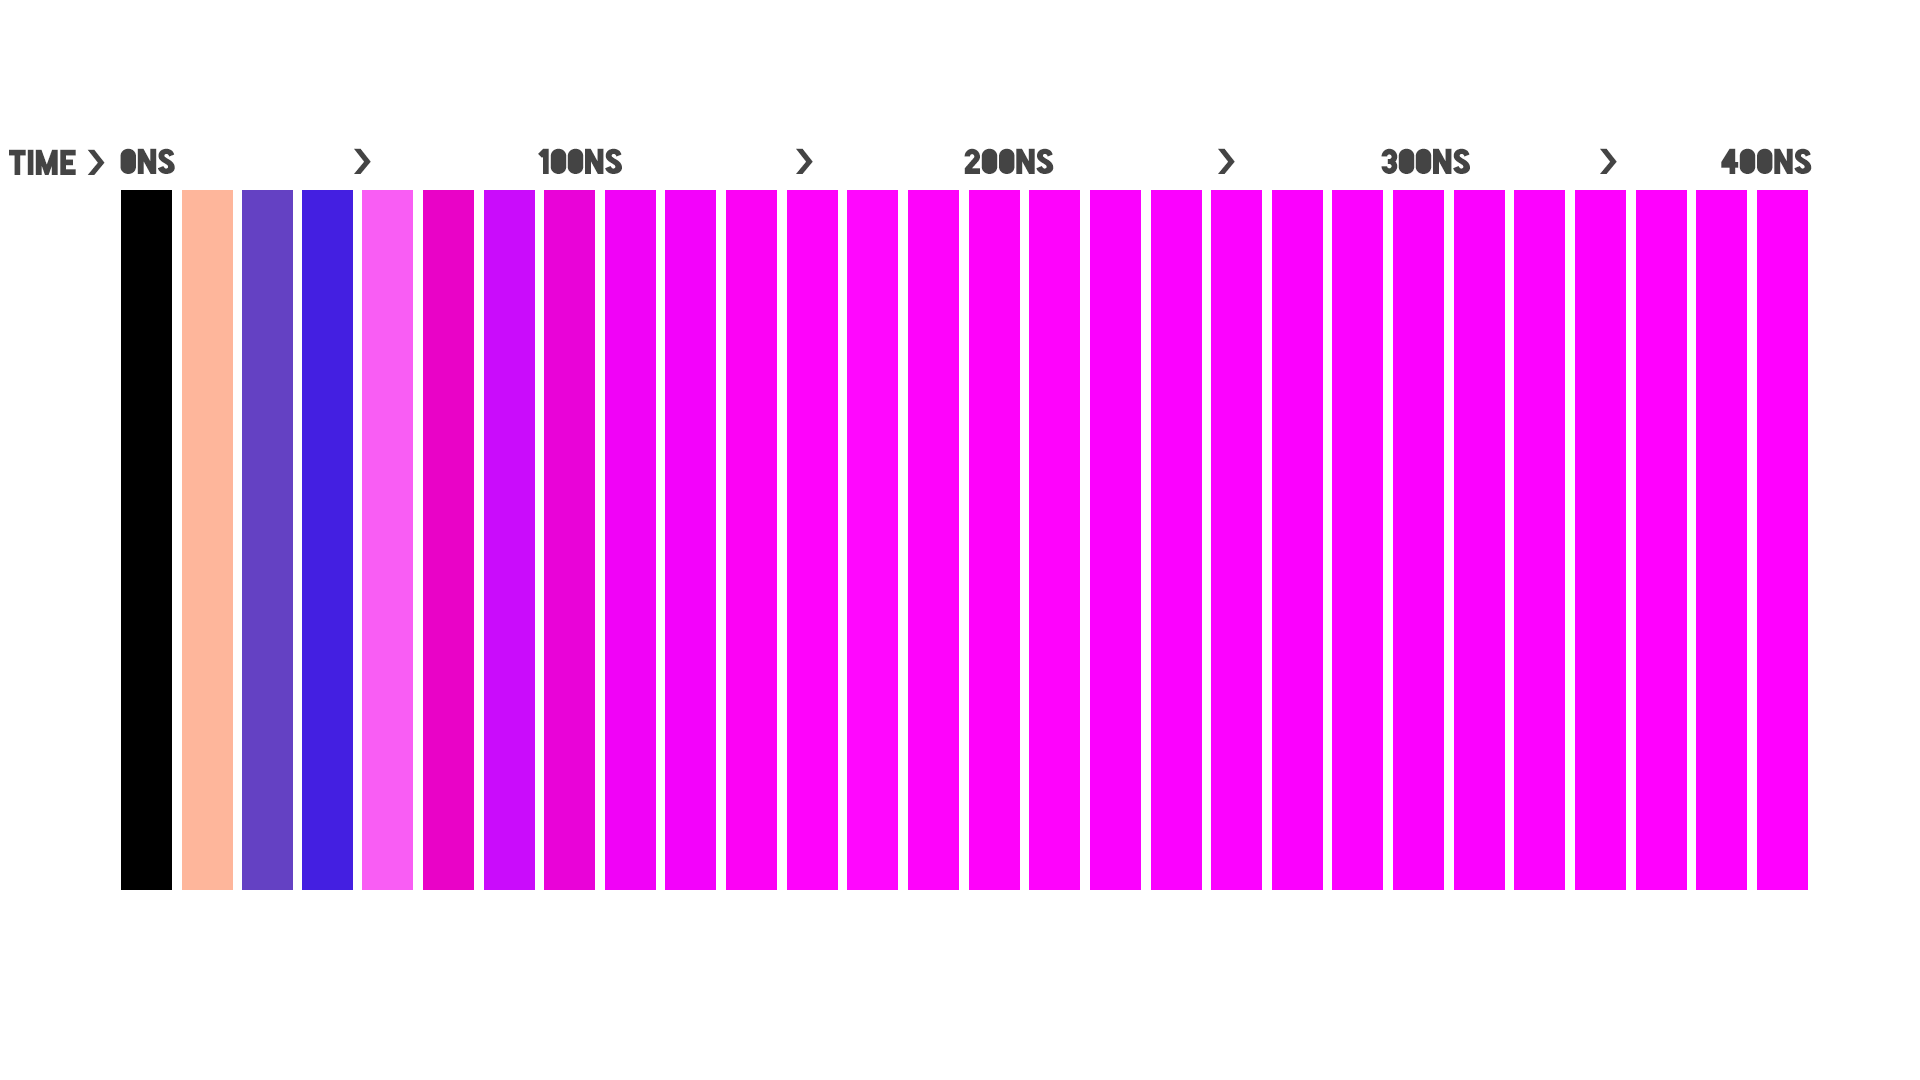
\includegraphics[width=\textwidth]{fig/color-search}
    \caption{Color search progression (7 cores, 1 core sampled)}
    \label{figure:color-search}
    \end{center}
\end{figure}

\subsection{Genetic Algorithm: Binary Knapsack Problem}

The knapsack problem is an optimization problem that is considered NP-hard.
The problem to solve is given a set of items with a weight and a value and a knapsack that can hold a specific weight, what combination of items that can fit in the sack has the highest value.
If there can be at most one of each item in the knapsack, we have what is known as the binary knapsack problem.

\subsubsection{Individual representation}

An individual represents a combination of items.
The individual is coded to a 64-bit data word like in Figure \vref{figure:binary-knapsack-bytefield}.

\begin{figure}[H]
    \begin{center}
        \begin{bytefield}[bitwidth=0.5em,endianness=big]{64}
            \bitheader{0, 63} \\
            \bitbox{63}{bit $ i $ set if item $ i $ is in the include set, else unset}
        \end{bytefield}
        \caption{The binary coding of an individual for the binary knapsack problem}
        \label{figure:binary-knapsack-bytefield}
    \end{center}
\end{figure}

\subsubsection{Fitness Function}
The fitness for an individual is calculated using Algorithm \ref{algorithm:binary-knapsack-fitness-function}.
The fitness falls between 0 for invalid sacks (that contain too much weight) to a theoretical maximum of the sum of the value of all the items.

\begin{algorithm}[H]
\SetAlgoLined
\DontPrintSemicolon
\KwData{A bit array with one bit representing whether each item is included or not}
\KwResult{How fit the individual is}
\Begin{
    $ weight \longleftarrow 0$\;
    $ value \longleftarrow 0$\;
    \For {item in ItemSet} {
        \If {item in genome} {
            $ weight \longleftarrow weight + item.weight$\;
            $ value \longleftarrow value + item.value$\;

            \If {$weight > maxWeight$} {
                $ value \longleftarrow 0$\;
                $ break $\;
            }
        }
    }
    \;
    \Return{$ value $}
}
\caption{The fitness function for the binary knapsack problem}
\label{algorithm:binary-knapsack-fitness-function}
\end{algorithm}

\subsubsection{Results}

This problem has not been run on the actual hardware, only simulated up to a few milliseconds.
The simulation seemed fine, and we got increasing fitness values, but the problem space is huge, so we probably need to run the algorithm for quite some time before coverging to a ideal/near-ideal solution.

\subsection{Blinkenlights}
Blinkenlights is a program that demonstrates the use of the input and output of the \Gls{barricelli} driven by the \Gls{SCU}.
When a button is pressed, the corrensponding LEDs to the button lit up.
This program is also described as a test for I/O, in \vref{iotest}, named Buttons \& LEDs.



\chapter{Discussion}
	\section{Performance}

The Barricelli computer is designed to be a device for high performance parallel computing.
Throughout the design process, choices have been made that further this goal.

The computer architecture is capable of executing multiple independent instruction streams working on multiple different independent data streams, which means that parallelism can be exploited to a large degree to achieve a high computational throughput.
A heterogenic collection of cores, some general, and some working as specialized accelerators, combines the allround-ness and usability of general computing with the at times extreme performance boosts given by specialized workers.

The general cores have been designed to exploit instruction-level parallelism, iwth features such as pipelining, hazard detection and correction using forwarding, and branch prediction.

The intelligent off-line assembler also helps off-load some of the hazard detection work from the processor, which lets the processor spend more of its valuable time computing.

Since the computer uses a shared memory bus though a single memory controller, it is an obvious scalability limitor.
For the instruction memory, this is somewhat mitigated by the inclusion of instruction caches, but there is still room for improvement.
To improve the memory performance, memory could be organized in a more hierarchical fashion, with multiple cache levels.

\subsection{Performance Measurements and Benchmarking}

With the specified prototype of the Barricelli computer presented in this report, looking at the results from the performance measurements in Chapter \vref{chapter:tests}, the optimal number of parallel fitness cores is 7.
Up to 7 processors, the performance scales beautifully, with calculated total performance scaling linearly with the number of cores.
After 7 cores, the relative performance of each core drops.
It is not easy to see exactly why this happens, but it is quite probably related to resource usage of the FPGA.

As the number of fitness cores increases, the more pressure it puts on the genetics accelerator.
As the number of fitness cores increases, the number of accelerators should also increase.

\subsection{Average Instructions per Cycle}

In optimal condititons, i.e.
the pipeline is filled, and no register spilling occurs, the processor can execute $ n $ instructions per cycle, where $ n $ is the number of processors.
In the designed protoype of Barricelli, this means that the maximum instructions per second is $ 7 cores * 50Mhz = 350 000 000 $, or 350 Mega-instructions per second.

\section{Theory}
In this section theory related to MIMD architectures and how to further improve their performances are discussed.
This also covers the discussions inside the group about the design of the architecture in the planning phase of the project.
\subsection{SPMD and Concurrency}
One of the first discussions that came up in the group after the assignment were given was if the processor cores should
be able to synchronize themselves.
By doing this, the processor cores would be able to execute code that is not completely independent in parallel in an elegant way.
However this also raises some issues as for instance data hazards.


\subsection{Using CISC or RISC ISAs}
CISC and RISC instruction set architectures are two very different ways of thinking when it comes to creating instruction sets.
While in the last years, RISC ISAs have been the most dominant instruction set architecture, we can also see that CISC architectures
are on their way back into the markets.
Some of the reasons for this is that increasing parallelism is gaining lesser performance increases.

\subsubsection{Micro Operations: a Bridge Between Complex and Reduced Instruction Sets}
The use of micro operations is based on the principle that you want to convert a complex instruction into a set of smaller micro operations.
This
may simplify the design of for instance a super scalar processor because dependencies between the converted micro instructions would already be known.


\subsection{Memory Management Policies}

The Galapagos architecture operates with several types of shared memory: \emph{instruction memory}, \emph{data memory}, \emph{instruction caches}, \emph{rated pool} and \emph{unrated pool}.
These types of memories  can further be divided into two groups: memory and genetic related.
These two groups are connected to separate data and address buses.
The access to these buses are handled by a request-acknowledgement protocol.
The responsible of this protocol is to control the access to the shared memories and their respective buses.
The protocol is based in the ideas of round-robin scheduling.
The request lines are continuously polled by the controllers in a round-robin fashion.
The reason for choosing this algorithm is because it is considered to be fair.
Since each request line is checked in turn, the algorithm is considered starvation free.
A requesting core will eventually get its request handled by the controllers.


Since all the cores access the same memories this solution will, however, turn out to be quite slow.
Note that every core is in fact competing for the access to memory.
For memory intensive problems this bottleneck will be quite visible.
Every time cores wishes to perform simultaneously some memory access only one of them will be granted access.
For instance, consider a system with five cores.
If these cores have a relatively frequent memory access pattern it pretty self explanatory that this will cause the the different cores being idle most of the time.
This will imply that the memory scheme in the galapagos architecture does not scale very well.
This implies that the more cores that are present the less performance would be achieved.


A possible solution for this problem would have been keeping separate data caches for each core.
Then the cores could have been using the data located in the caches instead of accessing the memory so frequently.
When first accessing the memory, the core could have loaded several data elements instead of just one word for each request.
This would surely been an improvement for the memory system employed in the baracelli currently.
This would, however, been very difficult to achieve, and is not in the scoop of this assignment.
Private data caches would require implementing cache coherence algorithms for keeping the caches consistent.
This is considered very difficult.



\subsubsection{Cache Coherency}
MIMD architecture use a shared memory models.
This imposes a problem when using caches, and memory in general.
When more core updates on the same values on the same memory positions; memory collisions occur.
These problems can be fixed by enforcing that only one core is able to access the memory at any given time.
A far more difficult problem is the problem of cache coherence.
Cache coherency issues occurs when several cores have private caches containing the same data, and some core changes the data.
Then the data in the caches is not consistent among the cores.
In order for the data to be consistent, in this example, is for each core having the same data.
Note that same data in this context mean data from the same memory location.


The Galapagos architecture does not support private data caches.
This design choice relieves the processor designer of implementing advanced cache coherency algorithms in hardware.
Instead of private data caches the Galapagos architectures employ shared pools for rated and un-rated chromosomes.
These are connected to a bus and the connected through the \emph{genetic controller}.
The controller is configured to only allow one core perform its operation on one of the pools at any given time.
This implies that read and write operations are atomic.
As a direct consequence cache coherency issues are not possible in the architecture.


\chapter{Work Process}
	\section{Development model}
For this project, it was agreed that an adaption of the Scrum development model should be used. The group wanted
to use an agile development method in order to be able to make quick changes to the requirement specification during the project.
The model is adapted however because many of the aspects in scrum, like working in sprints does not work so well for this project due to the unpredictable nature of the project. 
For the same reasons there was no daily meetings, but rather once in a week where everyone is informed about the current progress of the project.
\section{Group Organization}

From early on, the group divided itself into 3 work groups, focusing on three main areas: FPGA, PCB and IO.
This was done largely based on the fact that it has been done similarly in the years before\cn, and it seemed like a reasonable thing to do.
One advantage in doing this is that each work group can become more specialized in their respective fields compared to if everyone were to work equally on everything.
This allows for a more advanced execution in the project, which is a good thing.
The group member work group allocation can be found in table \vref{table:group-allocation}.

Other than this group allocation, no other hierarchical elements were introduced.
The group functioned as a direct democracy in all other issues, with no appointed leader. This approach had both
it's benefits and downsides. The greatest benefit is that everyone got to take part in the important decisions made in the project.
The downside was that decisions also take much longer time to take due to having to discuss matters over a meeting.


\begin{table}[H]
\begin{center}
\begin{tabular}{l}
\textbf{FPGA} \\
\hline
Sigve Sebastian Farstad \\
Torbjørn Langland \\
Per Thomas Lundal \\
Bjørn Åge Tungesvik \\
\\
\\
\textbf{PCB} \\
\hline
Fedor Fadeev \\
Eirik Flogard \\
Rune Holmgren \\
Odd Magnus Trondrud \\
\\
\\
\textbf{IO} \\
\hline
Emil Taylor Bye \\
Péter Gombos \\
\end{tabular}
\caption{Group Allocation}
\label{table:group-allocation}
\end{center}
\end{table}

The group held weekly sync-up meetings in addition to a weekly status meeting with the course staff.
Unfortunately, meeting attendance was occasionally some lower than what it should have been.
Fortunately, meeting minutes were always kept, so information from missed meetings did not go lost.

\section{Organizational tools}
\subsection{GitHub}
GitHub was used in order for everyone to be able to work at different parts of the project at the same time.
It also provides an excellent version control that would allow a user to work on experimental "branches". When using 
branches, the users does not need to worry about taking backups before trying out something new. These branches can also be merged into the main project later.
\subsection{Trello}
Trello is a tool that the group used as "scrum table" to keep everyone updated in real time about the current progress in the project.
The tool resembles a scrum board which keeps track of what everyone is doing at a specific time.

\section{Tools}
Below here is a list of tools that were used directly to develop the system.
\todo{a huge list of tools that we've used: compilers, IDEs, microscopes, 3d-printers, logic analyzers, software, websites, calculators. If we've used it, it's going in here, and it's going to be detailed.}

\todo{The following is more or less yanxed from dmkons, so we need to go over it and make sure that the numbers are all correct.}

\subsection{Software}
\begin{description}
    \item{\textbf{ISE Project Navigator 12.4 (nt64) M.81d, expired licence}} \\
        Main IDE for writing VHDL.
    \item{\textbf{ISim 12.4 (nt64) M.81d, expired license}} \\
        Main simulation environment for simulating VHDL.
    \item{\textbf{ModelSim SE 6.6d}} \\
        Secondary simulation environment for simulating VHDL.
    \item{\textbf{Xilinx Platform Studio 12.4 (nt64) Build EDK\_MS4.81d+1, expired licence}} \\
        Used for preparing compiled VHDL for the FPGA board.
    \item{\textbf{IAR Embedded Workbench for ARM 6.60.2.5507}} \\
        Used for programming and debugging on the microcontroller.
    \item{\textbf{Avnet Programming Utility}} \\
        Used for configuring the FPGA.
    \item{\textbf{energyAware Commander 2.82}} \\
        Programming and troubleshooting of the microcontroller.
    \item{\textbf{energyAware Designer 1.10}} \\
        Used for configuring the GPIO pins and generating projects for the microcontroller.
    \item{\textbf{Saleae Logic 1.1.9}} \\
        Used to view the sampled waveforms from the logic analyzer
    \item{\textbf{Tera Term Pro Web Version 3.1.3}} \\
        Terminal emulator used for serial communication.
    \item{\textbf{Text editors}} \\
        Sublime Text 2, Vim 7.3, Notepad (©Copyright Microsoft Corporation).
    \item{\textbf{GNU command-line tools}} \\
        Grep, sed, find, etc.
    \item{\textbf{git 1.8.1.2}} \\
        Version control system.
    \item{\textbf{GitHub}} \\
        Remote code repository hosting, issue tracking, wiki for logging.
\end{description}

\subsection{Hardware}
\begin{description}
\item{\textbf{Xilinx Spartan-6 XC6SLX45 CSG324}}
    FPGA board.
\item{\textbf{Energy Micro EFM32GG990F1024}}
    Microcontroller.
\item{\textbf{Energy Micro EFM32GG-DK3750}}
    Development kit used for testing code on the microcontroller before the PCB arrived.
\item{\textbf{Energy Micro EFM32GG-STK3700}}
    Prototyping and development when the microcontroller on the PCB could not be used.
\item{\textbf{Saleae Logic}}
    Logic analyzer
\item{\textbf{Development PC, Windows 7}}
    For development.
\item{\textbf{Mini USB cable}}
    For connecting the FPGA board to the development computer.
\end{description}


\chapter{Conclusion and \protect\\ Further Work}

\printglossaries

\part{Appendices}
	\appendix
\chapter{Galapagos Instruction Set Architecture Documentation} \label{appendix:isa}
\newpage
\includepdf[pages=-]{isa/isa.pdf}

\chapter{PCB schematics} \label{appendix:pcb-schematics}
\newpage

\chapter{Case schematics} \label{appendix:case-schematics}
\newpage

\chapter{Galapos Assembler Listing} \label{appendix:galapagos-assembler-source-code}
\newpage

\lstinputlisting[language=Python]{galapagos-assembler/galapagos/__init__.py}
\lstinputlisting[language=Python]{galapagos-assembler/galapagos/assembler.py}
\lstinputlisting[language=Python]{galapagos-assembler/galapagos/base.py}
\lstinputlisting[language=Python]{galapagos-assembler/galapagos/instructions.py}
\lstinputlisting[language=Python]{galapagos-assembler/galapagos/scanner.py}

\chapter{Demonstration Program Listings} \label{appendix:demonstration-programs-source-code}
\newpage

\chapter{Budget} \label{appendix:budget}
\newpage


\bibliography{reference-library}
\bibliographystyle{plain}
\nocite{*}

\end{document}
